%%%%%%%%%%%%%%%%%%%%%%%%%%%%%%%%%%%%%
%%%%%%%%%%%%%%%%%%%%%%%%%%%%%%%%%%%%%
%%
%% Typeset by                  , Research Press, NRC
%% Date: 
%% NRC, <name of journal>
%% 
%%%%%%%%%%%%%%
%%
%% 1. See original preamble material (at bottom of file) for
%%    details on source of current .tex file: conversion
%%    from word-processing program or author-generated TeX
%%    code. 
%%
%% 2. This template includes most options and packages used by 
%%    all the NRC journals. UNcomment those packages and options
%%    which are REQUIRED. 
%% 
%%%%%%%%%%%%%%%%%%%%%%%%%%%%%%%%%%%%%
%%%%%%%%%%%%%%%%%%%%%%%%%%%%%%%%%%%%%


%% 1. Class file (nrc1 or nrc2) + options (see userguide, pp.1-2; p.9):
\documentclass[%% french,        %% use with \usepackage[french]{babel}
               %% leqno,         %% only for nrc1 (default is right eqno)
               %% reqno,         %% only for nrc2 (default is left eqno)
nonumbib,      %% biblio entries without nos.
%
               %% breakaddress,  %% linebreak btwn author(s) + address(es)
               %% twocolid,      %% IDbox spans 2 cols
               %% twocolid*,     %% 2-col IDbox
               %% preprint,      %% removes identifying nos. from headers/footers
               %% proof          %% `Proof/Epreuve' in footer
               %% pagnf,         %% `Pagination not final/Pagination non finale'
               %% trimmarks,     %% add trimmarks
               %% finalverso,    %% final blank verso NOT included in pagerange
]{nrc1}                          %% choose one: nrc1 or nrc2

%% NOTE: authors may use the following options, which should be
%%       DELETED once the file comes in-house:
%%      
%%       usecmfonts    type1rest     genTeX

\usepackage{lineno}


\usepackage{color}
\newcommand{\red}{\textcolor{red}}

%% 2. Frequently used packages -- see pp.2-3 of userguide: 
%%    a. graphics-related:
\usepackage{graphicx}       %% color not usually needed
\usepackage[figuresright]{rotating} %% for landscape tables

%%    b. math-related: 
\usepackage{amsmath}        %% math macros in wide use
%%    \usepackage{amssymb}        %% additional math symbols
%%    \usepackage{dcolumn}        %% decimal alignment for tables
%%    \usepackage{bm}             %% `bold math' via \bm command

%%    c. for website addresses:
%%    \usepackage{url}            %% inserts linebreaks automatically
%%    \NRCurl{url}

%%    d. biblio-related:
%\usepackage{cite}           %% enhances options for \cite commands
\usepackage[authoryear, round]{natbib}

%%    e. for English-language papers:
\usepackage[french,english]{babel}  

%%    f. for French-language papers: 
%%    \usepackage[english,french]{babel}  %% remember to add french as a
                                          %% CLASS option, above
%%    g. for ragged-right tables:
%%    \usepackage{array}
%%    \newcommand{\PreserveBackslash}[1]{\let\temp=\\#1\let\\=\temp}
%%    \let\PBS=\PreserveBackslash

%%    h. for left curly brace to span several lines of equations:
%%    \usepackage{cases}
%%    \expandafter\let\csname numc@left\expandafter\endcsname\csname 
%%                 z@\endcsname


%% 3. Resetting float parameters: 
%%    a. in nrc1:
%%    \renewcommand{\topfraction}{.95}
%%    \renewcommand{\textfraction}{.05}
%%    \renewcommand{\floatpagefraction}{.95}

%%    b. in nrc2:
%%    \renewcommand{\topfraction}{.95}
%%    \renewcommand{\floatpagefraction}{.95}
%%    \renewcommand{\dbltopfraction}{.95}
%%    \renewcommand{\textfraction}{.05}
%%    \renewcommand{\dblfloatpagefraction}{.95}


%% 4. Resetting journal-specific parameters:
%%    a. eqn nos. with section nos.:
%%    \numberby {equation}{section}
%%    \setcounter{equation}{0}

%%    b. in-line citations to use ( ) instead of default [ ]:
%%   \renewcommand{\citeleft}{(}
%%   \renewcommand{\citeright}{)}

%%    c. for JEES (to expand inter-line spacing; see p.12 of guide):
%%    \easebaselines


%% 5. Miscellaneous macros to always have available:
%%    a. shorthands:
\let\p=\phantom
\let\mc=\multicolumn

%%    b. struts for vertical spacing above/below rules in tables:
%%%%%%%%%%%%%%%%%%  beginning of Claudio Beccari's code:
%% Spacing commands for {tabular} (from TTN 2,3:10 -- Claudio
%%                                                    Beccari): 
%% Usage: a. use \T to put space below a line 
%%           (e.g., at top of a `cell' of text)
%%        b. use \B to put space above a line 
%%           (e.g., at bottom of a `cell' of text)
\newcommand\T{\rule{0pt}{2.6ex}}            % = `top' strut
\newcommand\B{\rule[-1.2ex]{0pt}{0pt}}      % = `bottom' strut
%%%%%%%%%%%%%%%%%%  end of Claudio's code 

%%%%%%%%%%%%%%%%%%%%%%%%%%%%%%%%%%%%%   end of class and package 
%%%%%%%%%%%%%%%%%%%%%%%%%%%%%%%%%%%%%   options, additional macros


%% Journal-specific information for opening page -- pp.9-11 of guide:
%% a. numbers:
\setcounter{page}{1}             %% replace 1 with starting page no.
\volyear{XX}{2001}               %% volume, year of journal 
\journal{}                       %% jrnl. abbrev. (see App.A of guide)
\journalcode{}                   %% jrnl. acro    (see App.A of guide)
\filenumber{}                    %% NRC file number
%% \filenumber*{}                %% prefixes \filenumber to all page nos.
                                 %% NOTE: COMMENT OUT class options
                                 %%             pagnf
                                 %%             proof
                                 %%       once no longer needed


%% b. dates:
\received{}                      %% insert date, no period
\revreceived{}                   %% <same>
\accepted{}                      %% <same>
\revaccepted{}                   %% <same>
%% \IDdates{}                       %% <same>. Use for `Revised ...' etc.
%% \webpub{}                        %% insert date
%% \commdate{}                      %% <same>


%% c. miscellaneous:
%%   \assoced{}                  %% insert name of Associate ed.
%%   \corred{}                   %% insert name of Corresponding ed.
%%   \dedication{}               %% insert text as neede
%%   \abbreviations{}            %% insert as needed

\linespread{2}

\begin{document}

%% Reversed titlebar -- see p.11 of userguide:
%% \specialtitle{}      %% for black stripe + text + regular title
%% \specialtitle*{}     %% black stripe + text only




%% Title, Author(s), Address(es) -- see p.4 of userguide for 
%%    various options to save time and keyboarding, esp. where
%%    authors share same address(s). 

\title{Reframing Stock Assessment As Risk Management; An Management Strategy Evaluation for Atlantic Tuna
Risk is an uncertainty that matters.}

%% Author 1:
\author{Laurence T. Kell}        
\address{ICCAT Secretariat, C/Coraz\'{o}n de Mar\'{\i}a, 8. 28002 Madrid, Spain; ~Laurie.Kell@iccat.int; ~Phone: +34 914 165 600 ~Fax: +34 914 152 612.}
        
\author{Josetxu Ortiz de Urbina} 
\address{{Instituto Espa\~nol de Oceanograf\'{\i}a IEO- CO M\'{a}laga, Pto. Pesquero s/n, 29640 Fuengirola (M\'{a}laga), Spain; ~urbina@ma.ieo.es; ~Phone: +34 952 19 71 24 ~Fax: +34 952 46 38 08.}}

\author{Gorka Merino}            
\address{{AZTI-Tecnalia, Herrera Kaia Portualdea, 20110, Pasaia, Spain; ~gmerino@azti.es; ~Phone: +34 667 174 456 ~Fax: +34 94 657 25 55.}}

\author{Paul De Bruyn}           
\address{{ICCAT Secretariat, C/Coraz\'{o}n de Mar\'{\i}a, 8. 28002 Madrid, Spain.}}

\author{Haritz Arrizabalaga}     
\address{{AZTI-Tecnalia, Herrera Kaia Portualdea, 20110, Pasaia, Spain; ~gmerino@azti.es; ~Phone: +34 667 174 456 ~Fax: +34 94 657 25 55.}}

\author{George Tserpes}          
\address{{Hellenic Centre for Marine Research (HCMR), Institute of Marine biological Resources, P.O. Box 2214, 71003 Poros, Heraklion, Greece, tel: +30 2810 337851, fax: +30 2810 337820, e-mail: gtserpes@her.hcmr.gr}}


\shortauthor{Kell, et al.} %% for headers

%%%%%%%%
%% This line goes here in nrc1.
%% \maketitle			
%%%%%%%%


%% Abstract/Resume area -- see pp.5,12 of userguide:
\begin{abstract}

%\begin{description}
% \item[One or two sentences providing a basic introduction to the field, comprehensible to a scientist in any discipline.]
% \item[Two to three sentences of more detailed background, comprehensible to scientists in related disciplines.]
% \item[One sentence clearly stating the general problem being addressed by this particular study.]
% \item[One sentence summarising the main result (with the words “here we show” or their equivalent).]
% \item[Two or three sentences explaining what the main result reveals in direct comparison to what was thought to be the case previously, or how the main result adds to previous knowledge.]
% \item[One or two sentences to put the results into a more general context.]
% \item Two or three sentences to provide a broader perspective, readily comprehensible to a scientist in any discipline, may be included in the first paragraph if the editor considers that the accessibility of the paper is significantly enhanced by their inclusion. Under these circumstances, the length of the paragraph can be up to 300 words. (The above example is 190 words without the final section, and 250 words with it).]
%\end{description}

%The Precautionary Approach (PA) requires that undesirable outcomes be anticipated and measures taken to reduce the probability of them occurring. This requires determining how well management measures achieve their objectives given uncertainty, i.e. to manage risk. %, i.e. with respect to the ability to assess and manage stocks, given their intrinsic variability and the occurrence of environmental events inherent to the system. 
%We therefore define stock assessment, consistent with the PA, as the description of the characteristics of a 'stock' so that its biological reaction to being exploited can be rationally predicted and the predictions tested. This requires a move away from stock assessment to the management of risk. We provide an example of how to do this using Management Strategy Evaluation, i.e. by determining under what conditions a simple stock assessment method, based on biomass, can be used to achieve management objectives. Although such models have been criticised as being too simplistic to capture the actual population dynamics we show that they can meet our definition of stock assessment. %by providing advice on stock status relative to reference points and predict the response of a stock to management. 
%A consequence of the adoption of the PA is that many more stocks have to be assessed. %Which in turn has resulted in the use of integrated models that can utilise more sources of data and information and an increased number of stock assessments for data poor and knowledge limited stocks. Which resulted in many stock assessment models require priors for population parameters such as r (the population growth rate at low population size). In the case of biomass base models these are commonly derived from age  based models. 
%We also show that 
%the population parameters derived from biomass and age based models are not equivalent and that 
%it is more important to develop priors for reference points used to provide management advice than for population parameters, such as population growth rate, used in the stock assessment model. 

\end{abstract}

%\begin{resume}\end{resume}

\maketitle

\linenumbers
\linespread{2}


\begin{itemize}
 \item Introduction to the field, comprehensible to a scientist in any discipline.
 \item A more detailed background, comprehensible to scientists in related disciplines.
 \item Statement of the general problem being addressed by this particular study.
 \item Main result (with the words “here we show” or their equivalent).
 \item Explain what the main result reveals in direct comparison to what was thought to be the case previously, or how the main result adds to previous knowledge.
 \item Put the results into a more general context.
 \item Provide a broader perspective, readily comprehensible to a scientist in any discipline.
\end{itemize}

\newpage

% I’d note that life history arguments have been used to show that the Schaefer production model is probably not appropriate for tunas (e.g. Fisheries Research 61 (1), 145-149), and something like a Pella-Tomlinson with BMSY<0.5B0 is probably more realistic (primarily due to high steepness).  I would guess that admitting this asymmetry in the yield curve would admit that considerably lower levels of current depletion are possible.
%The authors should also justify why MSE was not used to evaluate the HCR. MSE can help in such situtations, as it can help add stability to the TAC decision process that industry can rely on rather than the whims of shifting political pressures. The stakeholder consultation is an essential part of the  MSE process. The MSE process can be used to guide the scientific process e.g. reducing many scientific uncertainties will make very little difference to the performance of a senisble feedback-based harvest control rule, but the simulation testing can help ensure that expenditure is priortized to provide the best research (or monitoring/enforcement) value.

\section*{Introduction}

%The objectives of fish stock assessment are to estimate stock status, to predict the response of a population to management and to validate the predictions to ensure that they are consistent with reality \citep{kell2015xval}. While a definition of risk is an uncertainty that matters \citep{hillson2010exploiting}. What matters depends on management objectives, and whether objectives are achieved depends on the management framework. For this reason management strategy evaluation \citep[MSE][]{kell2006operationa,punt2014management,carruthers2015simple} is increasingly being used to develop robust control mechanisms \citep[e.g.][]{rohrs1985robustness}. Where a robust system is one that still functions correctly in the presence of uncertainty or stressful environmental conditions \citep{radatz1990ieee}. A definition of uncertainty is the difference between models and reality \citep{chang2014robust} and a good model should be simple enough to facilitate the design of a control system, yet complex enough to give confidence that designs based on it will work on the true system \citep{zhou1996robust}.

%We are uncertain, to varying degrees, as much of the past is hidden from us, we have only limited information about the present and no knowledge of the future \cite{lindley2006understanding}. This is particularly true in fisheries science and management where uncertainties and the risks they create are pervasive owing to natural variability in components of aquatic ecosystems, imperfect information about those components, and lack of perfect control over fisheries \cite{peterman2004possible}. An important sources of uncertainty related to stock assessment modelling is \textit{structural uncertainty} due to inadequate models, incomplete or competing conceptual frameworks, or where significant processes or relationships are wrongly specified or not considered. Such situations tend to be underestimated by experts \cite{morgan1990uncertainty}. 

%Once we define stock assessment as ``The description of the characteristics of a 'stock' in such a way that its biological reaction to being exploited can be rationally predicted and the predictions tested'' then stock assessment is not just the estimation of current stock status but requires the development of robust control mechanisms even when system dynamics are unknown \citep[e.g.][]{rohrs1985robustness}. The accepted way to develop such control rules in fisheries is through MSE.

%In this study we show how to reframe stock assessment as risk management using  Management Strategy Evaluation (MSE) and an example based on tuna stocks managed by the International Convention for the Conservation of Atlantic Tuna (ICCAT).

%When managing fisheries decisions have to be made with incomplete knowledge, i.e. uncertainty about many processes . Therefore many fisheries organisations have adopted the Precautionary Approach \citep[PA,][]{garcia1996precautionary} which requires that undesirable outcomes be anticipated and measures taken to reduce the probability of them occurring. Risk is defined as \textit{an uncertainty that, if it occurs, will have an effect on objectives} \citep{hillson2011risk} and requires a proactive approach since to reduce risk requires managing the causes of uncertainty rather than just the consequences. In traditional stock assessment uncertainty may result in a lack of action \citep[e.g.][]{fromentin2014spectre}. Reframing uncertainty as risk is therefore consistent with the PA.

%MSE is used to determine how well management measures achieve their objectives given uncertainty, intrinsic variability and the occurrence of environmental events inherent to the system \citep{kirkwood1995assessing}. Therefore MSE can help in reframing stock assessment as risk management by evaluating what combinations of data, knowledge and algorithms to estimate stock status and set control measures best meet management objectives. 

%A consequence of the adoption of the PA is that stocks are assessed regularly with respect to limit reference points (LRPs). These indicate the state of a fishery or a stock considered undesirable and when fishing effort should be reduced so that are not reached \citep{gabriel1999review}. Target reference points (TRPs) may also be used to guide management and allow objectives such as achieving Maximum Sustainable Yield (MSY) to be met. The conventions of some Regional Fisheries Management Organisations (RFMOs) such as the ICCAT, however, were signed before the PA was drafted and so do not explicitly address the PA \citep{de2012precautionary}. The advice framework of ICCAT was originally based on achieving MSY; although limit reference points are now also being defined. This is in contrast to other scientific frameworks such as that of the International Commission for the Exploration of the Sea (ICES), which was originally based on LRPs and TRP are only now being incorporated. Scientific advice advice of the tuna RFMOs like ICCAT, who are responsible for the management of tuna and tuna like species in areas beyond national jurisdiction, is based on a common scientific advice framework \citep{kell2015kobe}. An exception is the Commission for the Conservation of Southern Bluefin Tuna CCSBT) which used MSE to develop an empirical harvest control rule \citep{hillary2015scientific}. 

%We define stock assessment as the description of the characteristics of a 'stock' so that its biological reaction to being exploited can be rationally predicted and the predictions tested. Under this definition MSE is an important tool to test predictive and management capability. The 'characteristics' of a stock are represented by the Operating Model (OM), a mathematical–statistical model used to simulate the resource dynamics and to generate monitoring data when projecting forward. MSE may be used to simulation test a Management Procedure (MP), which is the combination of pre-defined data, together with an algorithm to provide a value for a TAC or effort control measure. The MP may include a HCR and a stock assessment estimator, but does not have to for example CCSBT used MSE to develop a model free MP based on year to year changes and trends in empirical indicators. 

%An objective of MSE is to develop a robust control or management system rather than to identify a "best fit" to the available data, since stock assessment datasets typically do not contain information on key processes e.g. those that determine productivity \citep{kell2015srp}.  A robust system is one that still functions correctly in the presence of uncertainty or stressful environmental conditions \citep{radatz1990ieee}. 

%In traditional stock assessment is assumed that system dynamics are known and expressed in the form of a mathematical model and that a management control, such as a total allowable catch  (TAC) can be adjusted based on that knowledge. MSE in contrast involves the simulation testing of closed-loop feedback systems, based on a management procedure (MP), i.e. the combinations of data, knowledge and algorithms used to estimate stock status and set control measures. The algorithms used to estimate stock status are generally simpler than traditional stock assessments; \citep{geromont2014generic} showed that simple MPs can perform as least as well as conventional stock assessments. The specification of the OM is a key task, there are various ways to do this \citep{kell2006operational} but all require consideration of a range of hypotheses about resource dynamics \citep[e.g.][]{leach2014elicit}.

%Risk depends on the definition of uncertainty. Stock assessment working groups often focus on technical aspects related to modelling e.g. the defintions of \cite{rosenberg1994uncertainty} mainly focus on aspects that can be quantified in mathematical models. The characterisation of uncertainty is ultimately a pragmatic choice depending on the purpose of a particular application. There are other classifications of uncertainty, for example chapter 2, defines `statistical uncertainty` which includes the structural, process and observation uncertainties, and combines ‘model error’, ‘ structural uncertainty’ and ‘value uncertainty’ into ‘structural uncertainty’; then summarises the different sources based on those that can be reduced and those that are inherent to the system i.e.

\begin{description}
\item[Irreducible] aleatoric
\begin{itemize}
 \item Process
 \item Implementation
\end{itemize}
\item[Reducible] epistemic
\begin{itemize}
 \item  Statistical
 \item  Structural
\end{itemize}
\end{description}

%Linguistic sources of uncertainty which play a role in communication and elicitation, or uncertainty related to risk perception or vagueness and the possibly contradictory nature of management goals are also important\citep{regan2002taxonomy}. The national discourses about resource use, power dynamics among nations based on cultural, economic, and epistemic histories shape the way the problems of internationally shared resources are understood but these crucial differences are rarely articulated in the language of stock assessments. Uncertainties related to institutional and social norms are also important because they pertain to the very definition of a management problem which is a social construct first and foremost. 


\section*{Material and Methods}

The most useful conclusion from the range of studies in ecology and other fields is that maintaining multiple working hypotheses throughout the analysis is the most important guidance, that managers should identify policies that are robust to the range of alternative hypotheses (Schindler and Hilborn 2015), and that correlative evidence should be regarded a priori as weak support for causation. [Correlation and Causation in Fisheries and Watershed Management]

An experiment is done in a controlled environment conducted by researchers in a scientific laboratory about a hypotheses. A field experiment is an experiment carried out in the participant's natural everyday environment. In both cases, the researcher is still manipulating the independent variables (changing the thing that affects the dependent variables). The main differences are that in the lab experiment, the researcher is able to control most of the conditions in the the setting. For example, the researcher can control who is present, what the staff says, how long the experiment takes, and so on. In the field experiment, the researcher may not have control over any of those conditions, as for example, people not related to the experiment may come and go randomly, those people can say whatever they want, and so on. The lab experiment has more control and so can better isolate factors thought to be important in the outcomes, but may not be very much like the natural everyday environment, and so the results may not generalize to those natural everyday environments. The field experiment is the natural everyday environment, and so the results of the study are more likely to generalize. However the field experiment has less control and so it may be very difficult to determine what factors were important in explaining the outcome. 

\subsection*{Case Study}

%Stock assessment methods are often classified on their information and data requirements \cite[e.g.][]{smith2005harvest, smith2008experience}. The highest information/data-rich tier uses catch-at-age and research surveys and the lowest tier is when only life history and limited fishery data are available. Scientific advice used by the International Commission for the Conservation of Atlantic Tunas (ICCAT), the Regional Fisheries Management Organisation (RFMO) responsible for the management of tuna and tuna like species in the Atlantic and adjacent seas, is predominantly based on fisheries dependent data and catch biomass using biomass dynamic stock assessment models \cite[e.g.][]{prager1994suite, mcallister2000application}. 

%Although age based models are also used by ICCAT assessment working groups, a lack of confidence in the quality of size and age data \citep{fromentin2014spectre} means that in most cases these models are not used to provide advice. However age based models could be used to develop hypotheses about stock dynamics. 

%Eight out of the ten commercial stocks that the SCRS provides ICCAT management advice on are assessed using biomass dynamic models. Even if MPs are not developed for these stocks MSE can be used to ensure that this advice is robust and that risks are managed.

%A stock may be defined on an ecological, evolutionary, or operational basis \citep{waples2006invited}. In this study we assume the later and that there is no immigration or emigration and that a stock is homogeneous.

\subsection*{Management Strategy Evaluation}

%When running an MSE control actions from the HCR are fed back into an Operating Model (OM) that represents the system being managed so that its influence on the simulated stock and hence on future fisheries data is propagated through the stock and fishery dynamics. In engineering this is known as closed loop feedback control \citep{zhou1996robust}. Feedback relaxes the requirement of having to have an exact model of the system being managed since the effect of the control actions on the system are monitored and adjusted accordingly.

%However, traditional stock assessment advice mainly considers uncertainty about sampling and processes (e.g. recruitment) when uncertainty about the actual dynamics has a larger impact on achieving management objectives \citep{punt2008refocusing}. For this reason, Management Strategy Evaluation \citep[MSE][]{butterworth1999experiences,kell2003tuna,kell2006operational,punt2007developing,punt2014management,hillary2013sbthcr} and simulation modelling is increasingly been used to evaluate the robustness of advice frameworks to the main sources of uncertainty.
%that of the IOTC. Where in the determination of appropriate reference points and harvest control rules, consideration must be given to major uncertainties, including the uncertainty about the status of the stocks relative to reference points. IOTC will also assess through management strategy evaluation the performance of reference points, including any interim reference points, and of potential harvest control rules to be applied as the status of the stocks approaches the reference points. The scientific committee of the IOTC is therefore setting interim limit and target reference points for current use in defining limits and targets. MSE will then be used to evaluate the LRPs these as part of a HCR. The approach taken by the albacore working group allowed advice to be provided in the Kobe framework consistent with the Commission’s decision making policy for development and application of conservation and management measures (Rec. 11-13). In order to advance the Commission-SCRS dialogue, the Albacore WG provided information to the Commission on the basis of a range of interim HCR parameters, i.e. target fishing mortalities and biomass threshold (or buffer which if the stock fell below would result in fishing mortality being reduced). The HCR meets the Commissions policy objectives based on the assessment outcomes, e.g. 1) For stocks in the green quadrant of the Kobe plot, management measures shall be designed to result in a high probability of maintaining the stock within this quadrant. 2) For stocks that are in the upper right yellow quadrant of the Kobe plot (overfishing), the Commission shall immediately adopt management measures designed to result in a high probability of ending overfishing in as short a period as possible. 3) For stocks in the red quadrant of the Kobe plot (overfishing and overfished), the Commission shall immediately adopt management measures, designed to result in a high probability of ending overfishing in as short a period as possible and the Commission shall adopt a plan to rebuild these stocks, and 4) For stocks in the lower left yellow quadrant of the Kobe plot (overfished but no overfishing), the Commission shall adopt management measures designed to rebuild these stocks in as short a period as possible.

\citep{kell2015kobe,edwards2015book}


%When managing fisheries decisions have to be made with incomplete knowledge. The Precautionary Approach \citep[PA,][]{garcia1996precautionary} therefore requires that undesirable outcomes be anticipated and measures taken to reduce the probability of them occurring. The adoption of the PA by fisheries organisations requires that stocks are assessed regularly with respect to limit reference points (LRPs). LRPs indicate the state of a fishery or a stock considered undesirable and when fishing effort should be reduced so that are not reached \citep{gabriel1999review}. LRPs may be used along with target reference points (TRPs) to guide management to allow objectives such as achieving Maximum Sustainable Yield (MSY) to be met. 

%This requires determining how well management measures achieve their objectives given uncertainty, intrinsic variability and the occurrence of environmental events inherent to the system \citep{kirkwood1995assessing}. However, uncertainty sometimes causes management action to be delayed \citep[e.g.][]{fromentin2014spectre}. Reframing uncertainty as risk is therefore consistent with the PA and requires a proactive approach as most risk standards define risk as \textit{an uncertainty that, if it occurs, will have an effect on objectives} \citep{hillson2011risk}. To reduce risk requires managing the causes of uncertainty rather than the consequences. However, traditional stock assessment advice mainly considers uncertainty about sampling and processes (e.g. recruitment) when uncertainty about the actual dynamics has a larger impact on achieving management objectives \citep{punt2008refocusing}. For this reason, Management Strategy Evaluation \citep[MSE][]{butterworth1999experiences,kell2003tuna,kell2006operational,punt2007developing,punt2014management,hillary2013sbthcr} and simulation modelling is increasingly been used to evaluate the robustness of advice frameworks to the main sources of uncertainty. In engineering a robust control (or management) system is one that still functions correctly in the presence of uncertainty or stressful environmental conditions \citep{radatz1990ieee}. When running an MSE control actions from the HCR are fed back into an Operating Model (OM) that represents the system being managed so that its influence on the simulated stock and hence on future fisheries data is propagated through the stock and fishery dynamics. In engineering this is known as closed loop feedback control \citep{zhou1996robust}. Feedback relaxes the requirement of having to have an exact model of the system being managed since the effect of the control actions on the system are monitored and adjusted accordingly.

%There are various definitions of stock assessment, we define stock assessment as \textit{The description of the characteristics of a 'stock' so that its biological reaction to being exploited can be rationally predicted and the predictions tested}.  Under this definition MSE is an important tool to test predictive and management capability. The 'characteristics' of a stock are represented by the OM, which is then used to evaluate what combinations of data, knowledge and algorithms to estimate stock status and set control measures, i.e. a Management Procedure (MP) will best meet management objectives. Algorithms to estimate stock status in the MPs are generally simpler than traditional stock assessments and \citep{geromont2014generic} showed that simple MPs can perform as least as well as conventional stock assessments. The specification of the OM then becomes a key task, there are various ways to do this \citep{kell2006operational} but all require consideration of a range of hypotheses about resource dynamics. 

%MSE can help to provide stability and reduce risk if management objectives and how to evaluate how well alternative management strategies meet them are agreed through a dialogue between scientists and stakeholders. It can also guide the institutional process by identifying where the reduction of uncertainty will reduce risk and thereby help to ensure that expenditure is prioritised to provide the best research, monitoring and enforcement \citep{fromentin2014spectre}.

%We therefore use MSE to determine under what conditions simple stock assessment methods, based on biomass, can be used to manage stocks.  Biomass dynamic models have been criticised \cite[e.g.][]{maunder2003time} as being too simplistic to capture the actual population dynamics. However, if a simple model can provide advice on stock status relative to reference points and predict the response of a stock to management why use anything more complicated  \citep{ludwig1985age}?  For example the Pella-Tomlinson model is used to set catch limits for baleen whales by the IWC.  Neither the form of the model nor its parameters are meant to provide an accurate representation of the dynamics of the population. Rather, it has been demonstrated by MSE that when used as an integral part of a management strategy with a HCRs it allows the robust calculation and setting of catches limits \citep{butterworth1999experiences}. % {http://luna.pos.to/whale/gen_rmp.html}


\subsection*{Management Strategy Evaluation}

%All acronyms are tablulated in Table \label{tab:acronyms}.

Conducting an MSE involves a number of steps, \cite[i.e. after][]{punt2007developing}

\begin{enumerate}
 \item Identification of management objectives and mapping these to performance measures in order to quantify how well they have been achieved;
 \item Selection of hypotheses for the OMs;
 \item Conditioning of the OMs using data and knowledge and possible rejection and weighting of hypotheses;
 \item Identifying candidate management strategies and coding these as MPs, i.e.the combination of pre-defined data, together with an algorithm to which such data are input to set control measures;
 \item Projecting the OMs forward using the MPs as a feedback controller, i.e.where information about the gap between the actual and reference levels is used to alter the gap in some way \citep{ramaprasad1983definition}; and
 \item Agreeing the MP that best meets management objectives.
\end{enumerate}

\subsubsection*{Management Objectives} 

%a) Management objectives, such as maximizing average catch, minimizing inter-annual fluctuations in TAC levels, returning or maintaining the stock in the green quadrant of the Kobe plot, etc., taking into account the requirements of Rec. [11-13];

%b) Acceptable quantitative level(s) of probability of achieving and/or maintaining stocks in the green zone of the Kobe plot and avoiding limit reference points; and

%c) Timeframes for halting overfishing on a stock and/or rebuilding an overfished stock. 


%The original management objective of ICCAT is to provide the maximum continuing catch \citep{iccat2007basictext}, interpreted as using maximum sustainable yield (MSY) as a target. However, the United Nations Conference On Straddling Fish Stocks and Highly Migratory Fish Stocks \cite[UNFSA][]{un1995straddling} now defines $F_{MSY}$ (fishing mortality  associated  with $MSY$) as an upper limit. ICCAT has recently asked the Standing Committee on Research and Statistics (SCRS) to define  biomass limit reference points for some stocks and work has started on evaluating HCRs \citep{iccat2007swgsm}.

%To help provide consistency of advice across the Tuna RFMOs a common management advice framework \cite[i.e. the Kobe Framework ][]{de2012precautionary} has been developed with a main objective of keeping stocks above $B_{MSY}$ and fishing below $F_{MSY}$. This requires management strategies to be reported with respect to the probabilities of maintaining the stock above $B_{MSY}$ and fishing mortality below $F_{MSY}$. Advice on stock status is normally given in the form of a phase plot (Figure \ref{fig:hcr} with a green quadrant corresponding to the  target region (i.e. where the stock is neither overfished ($B \geq B_{MSY}$) nor subject to overfishing ($F \leq F_{MSY}$).

%Management advice is determined upon which quadrant a stock falls into. If the stock is in the green quadrant the objective is to maintain the stock in this state with high probability. While if the stock is in the red quadrant then management measures should be adopted immediately taking into account the biology of the stock and scientific advice to result in a high probability of ending overfishing in as short a period as possible (REC-11-13).

%Although often not explicitly specified social and economic objectives need to be considered \citep{iccat2007swgsm}. These may include minimising variability in catch and/or effort since wide annual fluctuations in catch and effort limit the ability of the fishing industry to plan for the future \citep{kell2005flat, kell2005round}. There will also be trade-offs between objectives, e.g. reducing variability in catches may require effort to be low. While some objectives may take precedence over others since without sustainability there will be no catch. 

%Quantifying how well management objectives are achieved is done using performance statistics, which are used to report on probabilities, risk levels, time scales and the power of the scientific advice framework to estimate stock status and to predict management performance. We consider five objectives (Table 1) and performance measures (Table 2) i.e. i) probability of being in the green quadrant; ii) average catch:$MSY$; iii) average Effort:(Effort at $F_{MSY}$); iv) average inter-annual variation (AAV) in catches expressed relative to $MSY$; and v) average inter-annual variation in Effort relative to Effort at $F_{MSY}$.

\subsubsection*{Operating Model} 

%The Operating Model scenarios are summarised in Table \ref{tab:grid} and those for the Observation Error Model in \ref{tab:oem}.  

%The management objectives and performance statistics are summarised in Tables \ref{tab:objectives} and \ref{tab:measures} respectively.


%When providing traditional stock assessment advice important sources of uncertainty are often underestimated by experts \citep{morgan1990uncertainty},  i.e. model error which includes structural uncertainty due to inadequate models, incomplete or competing conceptual frameworks, or where significant processes or relationships are wrongly specified or not considered. Even if the form of a process is known, the parameters may not be (i.e. value uncertainty) due to missing or inaccurate data or poorly known parameters. In ICCAT stock assessments there is uncertainty about biological parameters such as growth, maturity and natural mortality while the lack of age data means that stock recruitment relationships can not be fitted reliably \citep{leach2014elicit}. Therefore to evaluate the risk due to uncertainty about stock dynamics we conditioned the OM on hypotheses from a literature review of North Atlantic albacore (\textit{Thunnus alalunga}) \citep{santiago2005integrated, santiago2004dinamica} and life history theory \citep{gislason2010does}. 

%Life history parameters have been described for many taxonomic groups and biological parameters are often strongly correlated \cite[e.g.][]{blueweiss1978relationships,gislason2010does}. This allows us to draw general conclusions about the impact of uncertainty about processes on the performance of the MP and associated risks. 

%For conditioning the OMs a factorial design was used with factors with 2 levels (Table 3); where the factors represent alternative hypotheses about biological processes, i.e. growth,  maturity, natural mortality and recruitment and targeting of age classes (i.e. relative fishing mortality-at-age). The different factors and levels could have been weighted based on how well they are supported by the available data or following discussion with stakeholders \citep{leach2014elicit}. However as in this study we are mainly concerned with identifying the factors that affect the performance of the MP the results and analyses are presented without weighting.
 
%For growth and maturity two hypotheses are considered based on \citep{santiago2005integrated,santiago2004dinamica} and life history theory \citep{gislason2010does}. While for natural mortality (M), a process about which there is considerable uncertainty \citep{hamel2014method}, two hypotheses concerning the mortality of older ages were considered related to the functional form (i.e.  \citep{lorenzen2002density} and \citep{chen1989age}). 

%The main form of density dependence assumed in most fishery models is based on the stock recruitment relationship, although other processes \cite[e.g. M,][]{powers2014age} could have been considered, where at high stock levels survival of recruits declines. However, it is difficult to actually estimate stock recruitment relationships for most stocks. \cite{szuwalski2014examining} showed that the environment may more strongly influence recruitment than spawning biomass over the observed stock sizes for many stocks. We therefore included hypothesis that recruitment exhibits long term fluctuations \citep[i.e. red noise][]{ravier2001longterm} as well as those based on a S-R, i.e. Beverton and Holt or Cushing. 

%The Beverton and Holt stock recruitment relationship \citep{beverton_dynamics_1993} is derived from a simple density dependent mortality model where the more survivors there are the higher the mortality. It is assumed that the number of recruits (R) increases towards an asymptotic level ($R_{max}$) as egg production increases. In contrast \citep{cushing1973dependence} proposed a power-law stock recruitment relationship for stocks where resources are not locally limiting and recruitment continues to increase with increasing stock size, but at a decreasing rate. Stock recruitment relationships were reformulated in terms of steepness ($h$) and virgin biomass ($v$)  where steepness is the proportion of the expected recruitment produced at 20\% of virgin biomass relative to virgin recruitment  $(R_0)$. However, there is often insufficient information to allow its estimation from stock assessment\citep{issf2011steep} and so two values of steepness were assumed i.e. 0.7 and 0.9. Virgin biomass was set at 1000 Mt to allow comparisons to be made across scenarios.
 
%Uncertainty about the ages targeted by the fishery was modelled by changing the selection pattern, i.e. i) mature or juvenile, by  assuming the selection pattern is the same as the maturity ogive or the maturity ogive offset by 2 ages to the left; ii) flat topped or dome shaped selection. 

%The stock was initially fished at 20\% of $F_{MSY}$ then over a period of x years fishing effort increased annually until it was fished at twice $F_{MSY}$ at which point a recovery plan was implemented. This plan reduced F to the $F_{Target}$ in 5 years (Figure \ref{fig:hcr}) after which a HCR was used.

%The OM was conditioned so that the stock was originally in the green quadrant of the Kobe Phase plot and then effort (and fishing mortality) increased annually until it ended up in the Red quadrant (Figure \ref{fig:hcr}). Shortly after entering the red quadrant a recovery plan was implemented to reduce F linearly to the target. The MP then started in year 55 after the 5 year recovery period. This follows the general pattern of exploitation seen in ICCAT stocks.

\subsubsubsection*{Observation Error Model}

%The Management Procedure (MP) is based on a biomass dynamic model uses total catch biomass and catch per unit effort (CPUE) data. These data are sampled from the OM by the Observation Error Model (OEM),  the component of the OM that generates fishery-dependent and/or fishery-independent resource monitoring data.

%In the past the SCRS of ICCAT stock assessment working groups have tended to run stock assessment including all the available CPUE series. CPUE indices tend to be conflicting and this practice result is parameter estimates intermediate to what would be obtained from the data sets individually, and \cite{schnute1993analysis} showed the most likely parameter values are not intermediary but occur at one of the apparent extremes. Therefore a new procedure is being used by the SCRS; i.e. groups of indices that show similar trends are identified and these are these groups of CPUEs are run as separate assessment scenarios; then a hindcast is run (Kell et al. submitted) to distinguish signal from noise. Only those CPUEs which past the hindcast test are then used in the actual assessment. 

%A 30\% CV was chosen based on the Multifan-CL fits to the CPUE; no bias was found in the main longline CPUE or evidence of hyper-stability.  In most tuna stock assessments, due to the lack of fisheries independent data, commercial catch per unit effort (CPUE) is used as a proxy for relative abundance. CPUE standardisation is intended to allow for changes in operational procedures, which may result in increases in efficiency and catchability.  However, it has long been recognised that such time series may not accurately reflect trends in population abundance \citep[e.g.][]{beverton1993dynamics, harley2001cpue, maunder_interpreting_2006, mckechnie_longline_2013,polacheck2006tuna}. Particularly since factors that affect changes in the spatial distribution of populations and the allocation of effort in response to management and economic drivers can affect catch and effort independent of  stock abundance \citep[e.g.][]{paloheimo_abundance_1964, tidd2011exit}. While interactions between changes in oceanographic conditions and exploitation can drive spatial and temporal dynamics \citep[see][]{fromentin2013oceanographic,arrizabalaga2014habitat}. 
 
%We therefore adopt the MSE approach used by the Commission for the Conservation of Southern Bluefin Tuna (CCSBT) where robustness trials are conducted \citep{hillary2015scientific} based on hypotheses about the relationship between CPUE and stock abundance (Table \ref{tab:oem}). These are  i) positive bias in future longline CPUE due to a trend in catchability; and ii)  hyper-stability where there is nonlinear relationship between longline CPUE and abundance so that proportional changes in actual abundance are greater than those observed in the CPUE \citep{harley2001cpue}.

%Quota management for albacore has only been introduced recently and catches often are below the TAC landings are not thought subject to implementation error.
    

\subsubsection*{Management Procedure}

%The approach taken by ICCAT is that of the IOTC. Where in the determination of appropriate reference points and harvest control rules, consideration must be given to major uncertainties, including the uncertainty about the status of the stocks relative to reference points. IOTC will also assess through management strategy evaluation the performance of reference points, including any interim reference points, and of potential harvest control rules to be applied as the status of the stocks approaches the reference points. The scientific committee of the IOTC is therefore setting interim limit and target reference points for current use in defining limits and targets. MSE will then be used to evaluate the LRPs these as part of a HCR. The approach taken by the albacore working group allowed advice to be provided in the Kobe framework consistent with the Commission’s decision making policy for development and application of conservation and management measures (Rec. 11-13). In order to advance the Commission-SCRS dialogue, the Albacore WG provided information to the Commission on the basis of a range of interim HCR parameters, i.e. target fishing mortalities and biomass threshold (or buffer which if the stock fell below would result in fishing mortality being reduced). The HCR meets the Commissions policy objectives based on the assessment outcomes, e.g. 1) For stocks in the green quadrant of the Kobe plot, management measures shall be designed to result in a high probability of maintaining the stock within this quadrant. 2) For stocks that are in the upper right yellow quadrant of the Kobe plot (overfishing), the Commission shall immediately adopt management measures designed to result in a high probability of ending overfishing in as short a period as possible. 3) For stocks in the red quadrant of the Kobe plot (overfishing and overfished), the Commission shall immediately adopt management measures, designed to result in a high probability of ending overfishing in as short a period as possible and the Commission shall adopt a plan to rebuild these stocks, and 4) For stocks in the lower left yellow quadrant of the Kobe plot (overfished but no overfishing), the Commission shall adopt management measures designed to rebuild these stocks in as short a period as possible.

%The harvest control rule (HCR) used is shown in Figure~\ref{fig:hcr}; the brown line sets the harvest rate (y-axis) depending on the estimated stock biomass (x-axis). The black line is the replacement line, i.e. for a given stock biomass a harvest rate above the black line will cause the stock to decline and a harvest rate below the line will cause the stock to increase. The light blue line shows the simulated stock. For a given target harvest rate (i.e. the horizontal part of the HCR) the target biomass is given by the intersection of the two lines. If the stock declines below the break point (i.e. a trigger biomass or threshold biomass reference point) the harvest rate is reduced progressively to a minimum level of harvest rate at a biomass level equal to the LRP.

%Biomass dynamic models combine recruitment, growth and natural mortality into a three parameters population model i.e.  the intrinsic growth rate ($r$), carrying capacity ($K$) and shape of the surplus production curve ($p$).  It is assumed that recruitment is a linear function of stock and all individuals spawn at age 1, have the same body mass, and that M is constant. We use the term biomass dynamic rather than surplus production since surplus production can also be considered when using an age structured model \citep{hilborn_quantitative_1992}. 

%The biomass of a stock next year ($B_{t+1}$) is equal to the biomass this year $B_{t}$, less the catch ($C_t$) plus the surplus production ($P_t$) i.e. 

%\begin{equation}  B_{t+1}=B_{t}-C_{t}+P_{t}\end{equation}  

%$P$ is given by the Pella-Tomlinson surplus production function \citep{pella1969generalized}

%\begin{equation}\frac{r}{p}\cdot~B(1-(\frac{B}{K})^p)\end{equation}  

%The dynamics i.e. productivity, the response of the stock to perturbations, and reference points are determined largely by $r$ and the shape of the production function $p$; if $p=1$ then MSY is found halfway between 0 and K, as p increases MSY shifts to the right.


%Two values for each of the reference points were evaluated i.e.  $F_{target}$ (75\% and 50\% of $F_{MSY}$), $B_{trigger}$ (80\% and 60\% of $B_{MSY}$) and $B_{lim}$ (40\% and 30\% of $B_{MSY}$).  


\subsubsection*{Simulation}

%Often due to a lack of information and conflicting signals in the data stock assessment working groups fix, constrain or penalise some of the parameters being estimated. Therefore before conducting the MSE the impact of the assumptions made on the population parameters ($r$, $K$ and the shape of the production function) and $MSY$ based reference points of the OM. To do this we used the Base Case OM without feedback to generate data up to and including the recovery period; we then fitted the biomass dynamic model penalising the likelihood for each of the estimated parameter and reference points in turn using the OM values and a CV of 50\%. 

%The MSE was conducted in two stages. In the first stage the Base Case OM was run for all MPs to identify pathological or redundant MPs, that need not be considered further. In the second stage a subset of MPs were evaluated using all the OMs.

%Random numbers streams were identical across MSE runs to make it easier to distinguish between factors. 


\section*{Results}

%The impact of OM assumption on reference points and population parameters are summarised in Figure \ref{fig:popPar}. In all cases the production function was skewed to the left, this means that the Schaefer (Logistic) production model is probably not appropriate and that a Pella-Tomlinson form with BMSY<0.5B0 is probably more realistic. An asymmetric yield curve will also allow lower levels of current depletion to be possible as productivity will be less impaired at low biomass. Of all the life history parameters steepness had the biggest impact (e.g. on $r$ and $F_{MSY}$). 

%To understand the impact of misspecification of the production function a logistic production function was fitted to the OM scenarios for 1000 Monte Carlo replicates and the estimates of reference points and population compared with the OM values (red vertical line) in (Figures \ref{fig:sa1} for p=1 and \ref{fig:sa2} for p known). Rows correspond to the quantity that was penalised, columns show the quantity being estimated; red indicates where the estimated quantity was also penalised. 

%\subsection*{Counter Factuals}

%\subsection*{Comparison of Production Functions}


%The  biomass based (i.e. MP) production functions are compared with their age based (i.e. OM) equivalents in Figure \ref{fig:pFn}. The biomass based production curves can be derived by either fixed $r$ and $K$ and estimating $MSY$ and $B_{MSY}$ (1st column) or by fixing $MSY$ and $B_{MSY}$ (2nd column). In practice due to the difficulty of estimating the shape of the production function the logistic form is commonly assumed (i.e. p=1) by stock assessment working groups. Therefore we compare the production functions when the shape is known or p fixed at 1. If the production function is based on the OM values of r and K then $MSY$ is over estimated if p=1 and $B_{MSY}$ is overestimated if the correct shape is known. Production curves based on the reference points fit better over the range of biomass that would be seen in practice in a fishery managed at $B_{MSY}$.

%Estimates of r from age and biomass based model are inconsistent.

 
%\subsection*{Simulation without feedback}

%To understand the impact of misspecification of the production function on stock assessment parameter estimates and reference points estimated by the MP for a 1000 Monte Carlo simulations of the OM are compared with the OM values (red vertical line) in Figures \ref{fig:sa1} and \ref{fig:sa2},  where for p=1 and p is known respectively. Rows correspond to the quantity that was penalised, columns show the quantity being estimated; red indicates where the estimated quantity was also penalised. 

%Estimates show the greatest variability when unconstrained (1st row). When p=1 all many distributions are bi-modal. This is because the data are generated by an OM production function that is asymmetric, productivity is higher when the stock is below $B_{MSY}$. However, the stock assessment assumes that productivity does not vary depending on whether the stock is above or below $B_{MSY}$. It therefore fits either to the left or right-hand side of the production function. Bi-modality may cause problems in the assessment since the estimates may be biased (if they are from a local minimum), unstable (as more data become available results may flip to a new quite different solution) and conflicting (different indices give different solutions). However, this is less of a problem if the shape is known. 

%When the shape is known then quantities are in general better estimated, although some quantities may be biased, e.g. $F_{MSY}$ if r is penalised. Penalising K or $B_{MSY}$ have the same effect since $B_{MSY}$ is just a scaling of K when p is known. Since it is the reference points that are used in the MP, preferably these quantities should be well estimated. Without priors there is great uncertainty in all estimates and estimates are biased.

%An important result from this analysis (as shown by \ref{fig:sa2}) is that prior knowledge of the reference points $F_{MSY}$ and $B_{MSY}$ has a bigger effect on reducing bias and increasing precision than prior knowledge of r.

%\subsection*{Simulation with Feedback}

%\subsubsection*{Screening of MPs}

%To determine which MP options performed best prior to testing their robustness all MP options were run for the Base Case.  Figure 6 shows the probability of being in the green quadrant and Figure 7 yield relative to $MSY$ (median with interquartiles).  

%If being in the green quadrant is the primary management objective (Figure \ref{fig:ssGreen}) then only those HCRs that achieve an appropriate level of risk can be considered further. For example if managers specify that the probability of being in the green quadrant has to be greater than 0.6 then any points in the red area do not meet the management objective. A target F of 0.75$F_{MSY}$ when shape parameter is set to 1 fails to meet the management objective and so can be excluded from subsequent evaluations. The choice of biomass limit and trigger reference points show little impact of the primary objective and so choice of limit and trigger reference points could be based on the 2nd objective (i.e. level of yield). The best yield is given for an F of 0.75$F_{MSY}$ when the shape is known. I.e. there is an economic benefit of determining what the shape of the production function is. However, using priors for r or $F_{MSY}$ reduces catch. 

%Figure \ref{fig:tscatch} shows time series of yield relative to $MSY$, medians and interquartiles and two example simulations. It can be seen that summaries can give a very different impression from what is likely to happen. I.e. yields will be more variable than suggested by the median and 50\% of the time yield will be outside the inter-quartiles.

%\subsubsection*{Robustness Tests}

%To evaluate the robustness of the candidate MPs a limited set were run for all OMs, and a reduced set of MPs (i.e. 4 HCRs with 2 choices of $F_{target}$ and B limits$/$buffers and four stock assessment procedures  where p=1 or was known and no parameters or r penalised). 

%The five summary statistics are summarised in Figure \ref{fig:smry} in sets of five panels.  HCR options are by column and stock assessment options by row. The dots represent the OM, which are all considered equally likely, and the objective of the simulation is to test the robustness of the MP. The choice of MP is based on its robustness, i.e. does it in all cases, despite the uncertainty about the actual system dynamics, meet all management objectives? Therefore the MP chosen might not give the best performance for any OM. Based on this strategy for choosing the MP, the best MP would be for an F of 0.5$F_{MSY}$ when the shape of the production function is know, the use of priors for r or the choice of LRPs are not important in this case.


\section*{Discussion}

%An important stage of the MSE process is pre-agreeing OM hypotheses, their weightings and the criteria for choosing between MPs. Since once these are agreed the best MP is pre-determined, the task is then to find it. Given infinite computing power and resources all possible stock assessments and HCRs could be evaluated. However, it is easier to first evaluate the existing scientific advice framework and identify additional components such as LRPs and HCRs. This also has the benefit of providing a benchmark against which new alternatives can be compared. 
%Agreeing OM hypotheses and associated weights is potentially problematic and should avoid choices being influenced by management implications and therefore ideally be pre-agreed through informed discussion before any computations.  However, some flexibility could be allowed, for example to identify hypotheses that although plausible make little difference in terms of management implications and so need not be considered further \citep{ace2007report}.
%In stock assessment parameters that are difficult to estimate are often  assigned priors or fixed, for example population growth rate (r),  steepness of the stock recruitment relationship or natural mortality \citep[e.g.][]{michielsens2004bayesian}. 
%An important result from this study is that prior knowledge of the reference points $F_{MSY}$ and $B_{MSY}$ has a bigger effect on reducing bias and increasing precision than prior knowledge of r. In most biomass based stock assessments when priors for r are used these are obtained from on age based models, this study showed that r from age and biomass based model are inconsistent and using priors for r may bias the reference points.
%Given our definition of Risk as \textit{an uncertainty that, if it occurs, will have an effect on objectives} the aim of risk management is to address uncertain events or conditions, in order  to stop negative risks from happening if possible, or at least to reduce their probability and/or impact \citep{hillson2011risk}. MSE can do this by showing where improving   management (i.e. through Monitoring Control and Surveillance) and knowledge (scientific research) can ensure that management objectives are met. A strength of MSE is that it should add stability to the management decision process as management objectives, and how to evaluate how well alternative management procedures meet them given uncertainty, are agreed through a dialogue between scientists, managers and stakeholders \cite[e.g.][]{rockmann2012added,fromentin2014spectre}. As part of the implementation of any management plan uncertainty related to how results are used also need to be considered \citep{francis54c}. I.e. \textit{Translational uncertainty} relating to explaining uncertain results and \textit{institutional uncertainty} where there is a lack of ways to handle these types of problems. To reduce uncertainty will not just require developing and running more models but developing a dialogue between stakeholders on issues such as acceptable levels of risk, time horizons and social and economic as well as biological targets and limits. The example MSE here based on albacore can be used for this purpose.

%In the case of biomass based stock assessment models priors are commonly derived from age  based models. However, population parameters derived from biomass and age based models are not equivalent and that it is more important to develop priors for reference points used to provide management advice than for population parameters.


\newpage
\section*{Conclusions}

%To quote \citep{adams2007risk} \textit{In the area lit by the lamp of science one finds risk management problems that are potentially soluble by science. Such problems are capable of clear definition relating cause to effect and characterized by identifiable statistical regularities. On the margins of this area one finds problems framed as hypotheses and methods of reasoning, such as Bayesian statistics, which can guide the collection and analysis of further evidence. As the light grows dimmer the ratio of speculation to evidence increases. In the outer darkness lurk unknown unknowns. We are in danger of becoming the drunk looking for his keys, not in the dark where he dropped them, but under the lamp post where there was light by which to see}. 
%To frame this as stock assessment, a huge effort appears to be going into estimating more parameters and conducting assessments for more and more stocks but without being able to relate cause and effect. This is partly since more stocks now need to be assessed which has resulted in two trends, i.e. the development of integrated models and general frameworks that can be applied to all stocks utilise a variety of sources of data and and estimate thousands of parameters, and the requirement to assess all stocks even when the quality of data and knowledge of population processes is poor. This often requires the use of Bayesian priors or fixing key parameters since otherwise stock assessment models do not converge due to parameters being highly correlated, ill-defined and/or assumptions violated.
%An alternative view is that of Sidney Holt (pers comm.) \textit{People should not be doing stock assessments (except maybe for fun) but, rather, assessment models of managing fishing as the real need is to model fisheries. The default is how a fishery grows and dies when we don't 'manage' it, and it is against that that one judges what are the likely consequences of an interference measure by us. Doing either of these you soon can see what really matters in any detail within the stock assessment bit, and it is much less than most people assume}


%The RMP of the IWC at its core a crude Pella-Tomlinson population model that nobody believed was remotely good as a population model. But it had the general properties that seemed to be relevant to the problem.} 
%Partly for these reasons \citep{hilborn2003state} argued that basing management decisions on simple feedback rules and assessments evaluated using MSE is preferable. Which like Bayesian method can guide the collection and analysis of evidence \citep{fromentin2014spectre}. A  benefit of framing stock assessment as risk management using MSE is that the identification of management objectives and quantify how well different actions achieve those objectives becomes the main area of discussion (MSE step 1). Unknown unknowns are addressed by conditioning OMs (MSE step 3). Reframing stock assessment as risk management also places the emphasis on robustness, i.e. does a management strategy  meet the agreed management objectives despite uncertainty (MSE step 6)?
%There are different definitions of risk, i.e. as effect or uncertainty. In the former case risk management focuses on how to avoid or minimise negative impacts and to exploit or maximise positive impacts. In the latter the aim is to address uncertain events or conditions which means to stop negative risks from happening where possible, or at least to reduce their probability and/or impact and to capture positive risks and maximise their probability and/or impact. Addressing uncertainty therefore leads to a more proactive approach than trying to tackle the effect \citep{hillson2011risk}. MSE can do this by identifying where the reduction of uncertainty will reduce risk and thereby help to prioritised to research, monitoring and enforcement \citep{fromentin2014spectre} and hence excorcise the spectre.

%Risk is now widely agreed to be double-sided and covers both upside and downside. However  ISO31000 “Risk management – Principles and guidelines” standard (published in November 2009) states that “Risk is effect…”  while everyother risk standard as  “an uncertainty that, if it occurs, will have an effect on objectives”. This is completely different from the ISO31000 risk definition. The other risk standards clearly state that a negative risk is an uncertainty that would cause delay or overspend or reputation damage if it happened. An upside risk is also uncertain and its occurrence would result in time or cost savings, or improved reputation. A risk can be an uncertain event or an uncertain set of circumstances or an uncertain assumption, but the key point according to these standards is that the risk is uncertain. Of course because a risk is uncertain then it may never happen, but if it does happen then it will have an effect on objectives. But the risk is not the effect. The risk is the uncertainty that would result in an effect.

%ISO would define the following as negative risks: delay, overspend, accidents, reputation damage, lost market share, inefficiency etc. On the upside we would see time or cost savings as positive risks, or enhanced performance or increased shareholder value. All of these things are effects on objectives that could arise from uncertainty.

%This matters because it determines the goal of risk management. If “Risk is effect…” then risk management seeks to manage those effects, and the risk process must focus on how to avoid or minimise negative impacts and how to exploit or maximise positive impacts. But if “Risk is uncertainty…” then the aim of the risk process is to address uncertain events or conditions. This means to stop negative risks from happening if possible, or at least to reduce their probability and/or impact. It also means to capture positive risks or maximise their probability and/or impact. Addressing the uncertainty leads to a more proactive approach than trying to tackle the effect.


\section{Acknowledgement}

This study does not necessarily reflect the views of ICCAT and in no way anticipates the Commission's future policy in this area. 

\newpage\clearpage
\bibliography{refs}
\bibliographystyle{abbrvnat}


\newpage\clearpage
\section*{Tables}
\begin{table}
\label{tab:grid}
\caption{Operating Model Scenarios; Base Case values in bold.}  
\begin{center}
\label{tab:datasumm}
\begin{tabular}{|cccc|}
\hline
			& {\tiny Levels (N)} & {\tiny $\prod$ N} & {\tiny Values} \\ %& {\tiny Prior} & {\tiny Weighting}\\
\hline\hline
{\tiny stock recruitment relationship} 	 & {\tiny 2} 	 & {\tiny   2}  & {\tiny  \textbf{Beverton and Holt}; Cushing}     \\                  & {\tiny ?}    & {\tiny ?}\\
{\tiny Steepness}	                 & {\tiny 2} 	 & {\tiny   4}  & {\tiny  \textbf{.9}; .75}                             \\
{\tiny $M$} 		                 & {\tiny 2} 	 & {\tiny   8}  & {\tiny  \textbf{Lorezen}; Chen \& Watanabe} 	        \\
{\tiny $Growth$} 	                 & {\tiny 2} 	 & {\tiny  16}  & {\tiny  \textbf{N. Atl. Life History}; Slower growth} \\
{\tiny $Maturity$} 	                 & {\tiny 2} 	 & {\tiny  32}  & {\tiny  \textbf{N. Atl.}; Life History}               \\
{\tiny Selectivity I}	                 & {\tiny 2} 	 & {\tiny  64}  & {\tiny  \textbf{as Mat}, domed}      		        \\
{\tiny Selectivity II}	                 & {\tiny 2} 	 & {\tiny 128}  & {\tiny  \textbf{as Mat}, juvenile}   		        \\
{\tiny Autocorrelation}	                 & {\tiny 2} 	 & {\tiny 256}  & {\tiny  \textbf{0}; 0.3}                              \\

\hline
\end{tabular}
\end{center}
\end{table}


\begin{table}
\label{tab:oem}
\caption{Observation Error Model Scenarios; Base Case values in bold.}  
\begin{center}
\label{tab:datasumm}
\begin{tabular}{|cccc|}
\hline
			& {\tiny Levels (N)} & {\tiny $\prod$ N} & {\tiny Values} \\ 
\hline\hline
{\tiny Trend in catchability } & {\tiny 2} 	 & {\tiny   2}  & {\tiny  \textbf{None}; 50\%}   \\
{\tiny Hyperstability}	       & {\tiny 2} 	 & {\tiny   4}  & {\tiny  \textbf{1}; 0.75}     \\
\hline
\end{tabular}
\end{center}
\end{table}


\begin{table}[h!]
  \label{tab:objectives}
  \caption{Management Objectives}  
  \begin{center}
    \begin{tabular}{ l p{10cm} }
    \hline
    Rule & Definition \\
    \hline 
     O1   & Maintain the stock in the \emph{green kobe quadrant}\\
     O2   & Achieve the maximum continuing catch \\
     O3   & Maintain high employment \\
     O4   & Stability of yield \\
     O5   & Stability of effort \\
     \hline
    \end{tabular}
  \end{center}
\end{table}

\begin{table}[h!]
  \label{tab:measures}
  \caption{Performance Statistics}  
  \begin{center}
    \begin{tabular}{ l p{10cm} }
    \hline 
    Statistic & Definition \\ 
    \hline 
    P1   & Probability of SSB $\geq$ $B_{_{MSY}}$ and F $\le$  $F_{_{MSY}}$ \\ 
    P2   & Catch\\ 
    P3   & Effort\\ 
    P4   & AAV Catch  \\ 
    P5   & AAV Effort  \\ 
    \hline 
    \end{tabular}
  \end{center}
\end{table}


\begin{table}[h!]
  \label{tab:acronyms}
  \caption{Acronyms}  
  \begin{center}
    \begin{tabular}{ l p{10cm} }
    \hline 
     & Definition \\ 
    \hline 
       &  \\ 
    \hline 
    \end{tabular}
  \end{center}
\end{table}

\newpage\clearpage
\section*{Figures}

\begin{figure*}[htbp]
\centering
\includegraphics[width=6in]{kobeHcr.png}
\label{fig:hcr}
\caption{Harvest Control Rule (brown) plotted on a phase plot of harvest rate relative to $F_{MSY}$ and stock biomass relative to $B_{MSY}$;
 the black line is the replacement line.}
\end{figure*}


\begin{figure*}[htbp]
\centering
\includegraphics[width=6in]{pcaSS.png}
\label{fig:pcaSS}
\caption{Principle component analysis of integrated model grid.}
\end{figure*}


\begin{figure*}[htbp]
\centering
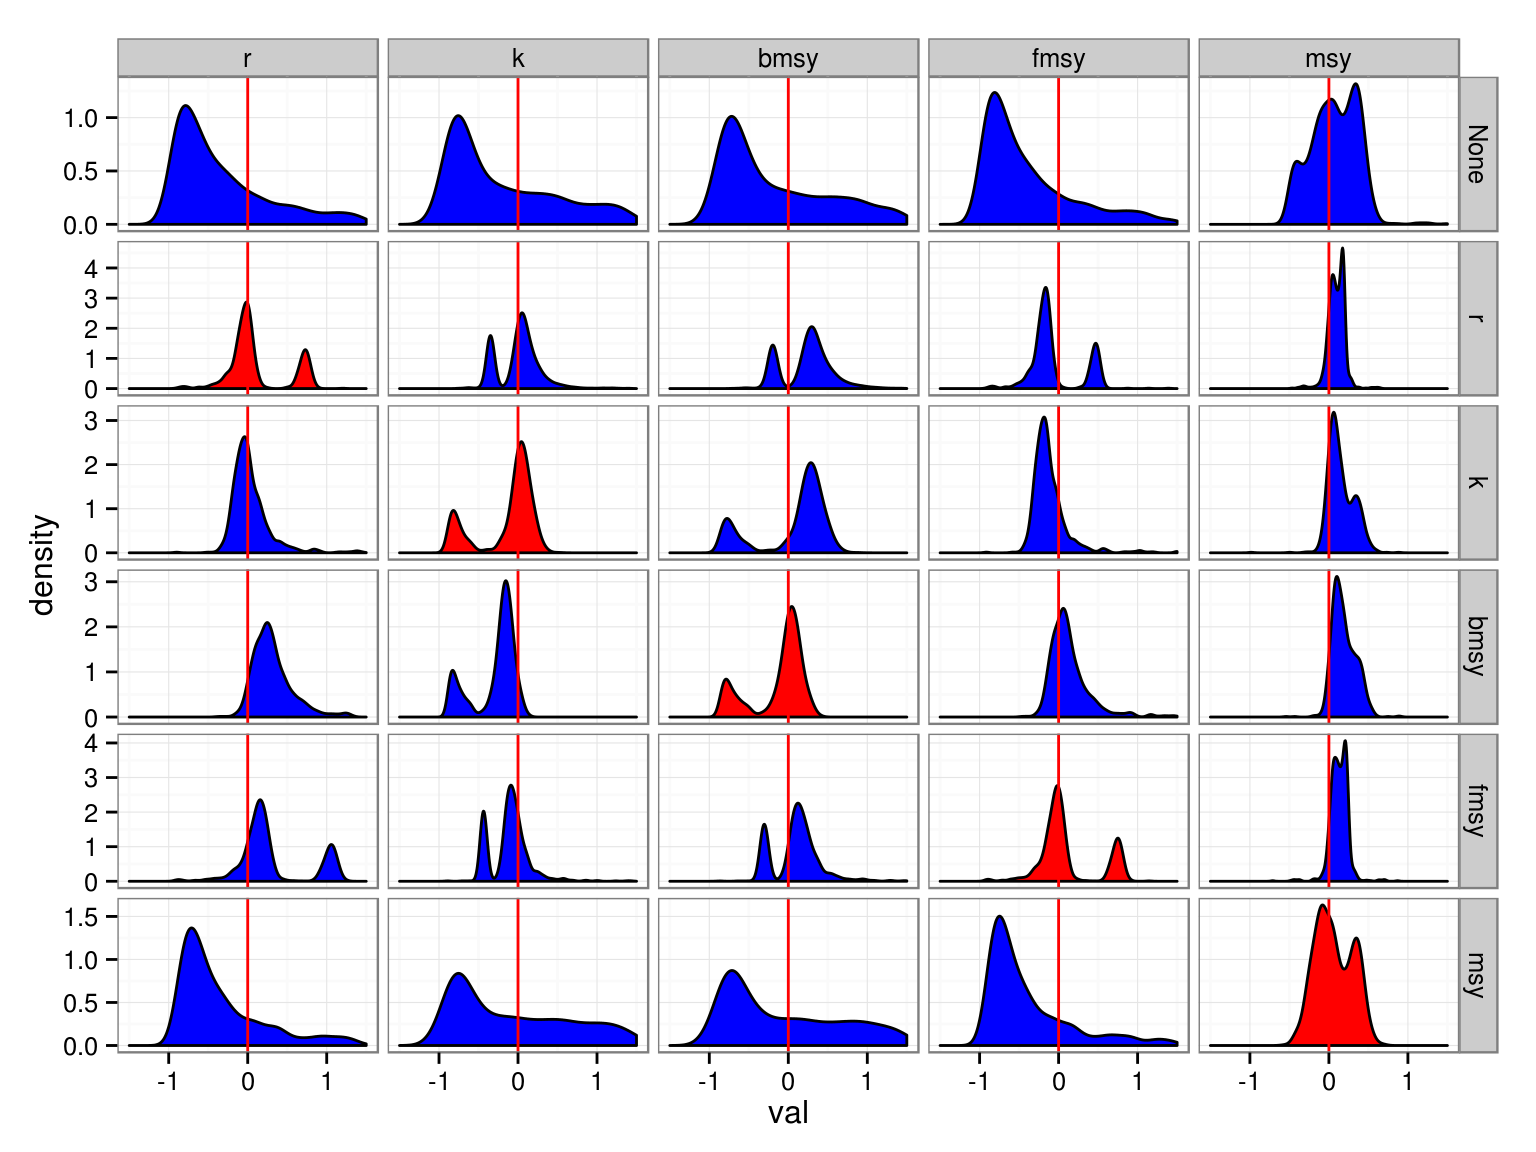
\includegraphics[width=6in]{SA1.png}
\caption{Estimated distributions of reference points and population parameters from the biomass dynamic assessment model for the Base Case OM, where the production function is assumed to be symmetric (p=1); the value penalised in the likelihood based on the OM value is given by row.}
\label{fig:sa1}
\end{figure*}

\begin{figure*}[htbp]
\centering
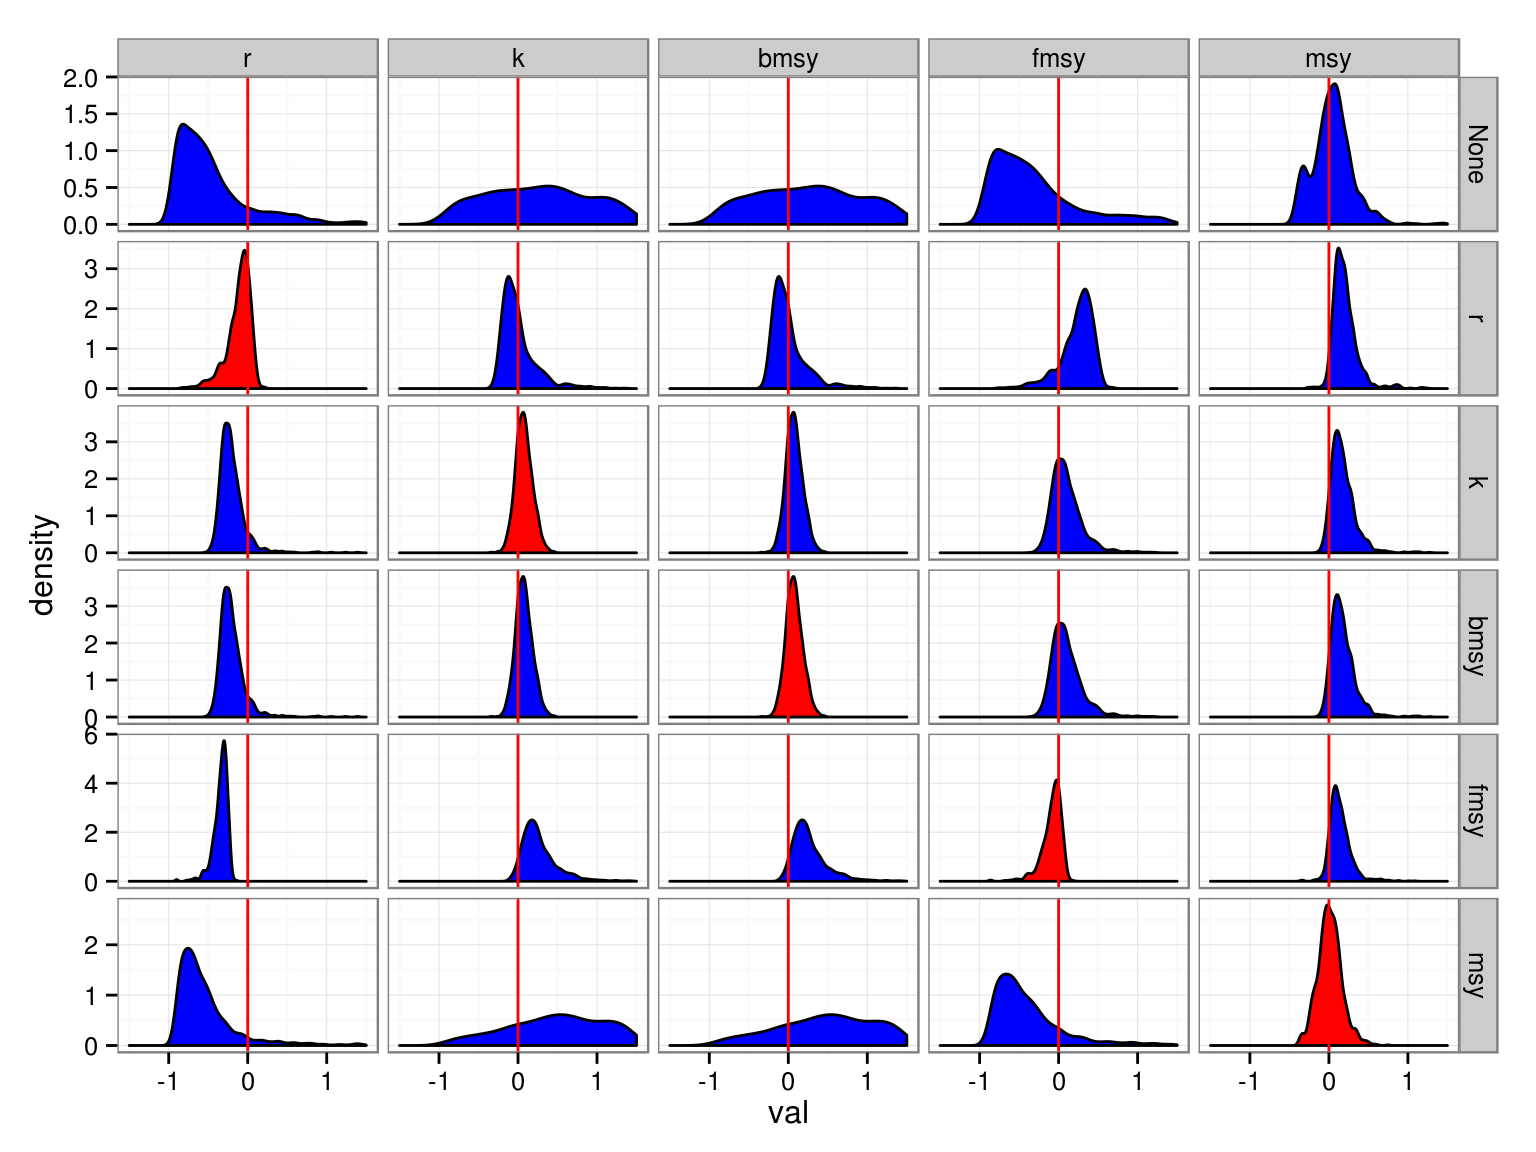
\includegraphics[width=6in]{SA2.png}
\caption{Estimated distributions of reference points and population parameters from the biomass dynamic assessment model for the Base Case OM, where the production function has the same shape as the OM (p=0.223); the value penalised in the likelihood based on the OM value is given by row.}
\label{fig:sa2}
\end{figure*}

\begin{figure*}[htbp]
\centering
\includegraphics[width=6in]{transfer1.png}
\caption{}
\label{fig:t1}
\end{figure*}

\begin{figure*}[htbp]
\centering
\includegraphics[width=6in]{transfer2.png}
\caption{}
\label{fig:t2}
\end{figure*}

\begin{figure*}[htbp]
\centering
\includegraphics[width=6in]{transfer3.png}
\caption{}
\label{fig:t3}
\end{figure*}

\newpage\clearpage
\section{Appendix}

\newpage\clearpage
\section*{Equations}

\subsection*{Operating Model}

Growth was modelled by the \cite{vonbert1957quantitative} growth equation i.e.
 
\begin{equation} L_t = L_{\infty}(1 - e^{-kt-t_0}) \end{equation} 
 
where $L_{\infty}$ is the asymptotic length attainable, $k$ the rate at which the rate of growth in length declines as length approaches
$L_{\infty}$, and $t_{0}$ is the time at which an individual is of zero length. 
 
Mass-at-age is then derived from length using a scaling exponent ($a$) and the condition factor ($b$)
 
\begin{equation} W_t = a \times W_t^b \end{equation} 
 
Maturity ($Q$) was either based on \cite{santiago2004dinamica}  or derived as in \cite{williams2003implications} 
from the theoretical relationship between $M$, $K$, and age at maturity ($a_{Q}$)  
based on the dimensionless ratio of length at maturity to asymptotic length \citep{beverton1992patterns}. It was then  
modelled by the logistic equation with 2 parameters: age at 50\% ($a_{50}$) and 95\% ($a_{95}$) mature.

\begin{equation}
f(x) = \left\{ \begin{array}{ll}
			0                                 &\mbox{ if $(a_{50}-x)/a_{95} >  5$} \\
			a_{\infty}                        &\mbox{ if $(a_{50}-x)/a_{95} < -5$} \\
			\frac{m_{\infty}}{1.0+19.0^{(a50-x)/{a95})}} &\mbox{ otherwise}
		\end{array}
       \right.
\end{equation}

Natural mortality ($M$) at-age was derived from \cite{lorenzen2002density} and \cite{chen1989age}, i.e.

for Lorenzen
 
\begin{equation}
   M_t=3.00*W_t-0.288
\end{equation}
   
   and Chen-Watanabe
 
\begin{equation}
M_t = \left\{ \begin{array}{ll}
			 \frac{k}{1-e^{-k(t-t_0}}     			&\mbox{ for $t<t_m$} \\
			\frac{k}{a_0}+a_1(t-t_m)+a_2(t-t_m)^2           &\mbox{ for $t<t_m$} \\
		\end{array}
       \right.
\end{equation}

where

\begin{subequations}
$a_0=1-e^{-k(t-t_0)}$  \\
$a_1=ke^{-k(t-t_0)}$ \\  
$a_2=-0.5k^{2e^{(-k(t-t_0))}}$ \\  
$t_m=\frac{1}{k}log(1-e^{-kt_0}) +t_0$ 
\end{subequations} 
 
Selectivity was modelled using a double normal \citep[see][]{hilborn2000documentation} with three parameters that describe the age at maximum selection ($a1$), the rate at which the left hand limb increases ($sl$) and the right hand limb decreases ($sr$) which allows flat topped or domed shaped selection patterns to be chosen.

\begin{equation}
f(x) = \left\{ \begin{array}{rl}
 2^{-[(x-a_1)/s_L]^2} &\mbox{ if $x<a_1$} \\
 2^{-[(x-a_1)/s_R]^2} &\mbox{ otherwise}
       \end{array} \right.
\end{equation}

Stock recruitment relationships were either \citep{cushing1973dependence}
\begin{equation} R=aS^b \end{equation}

or Beverton and Holt \citep{beverton_dynamics_1993}

\begin{equation} R=\frac{S}{a+bS} \end{equation}

\subsection*{Observation Error Model}


\subsection*{Management Procedure}

The biomass of a stock next year ($B_{t+1}$) is equal to the biomass this year $B_{t}$, less the catch ($C_t$) plus the surplus production ($P_t$) i.e. 

\begin{equation}  B_{t+1}=B_{t}-C_{t}+P_{t}\end{equation}  

$P$ is given by the Pella-Tomlinson surplus production function \citep{pella1969generalized}

\begin{equation}\frac{r}{p}\cdot~B(1-(\frac{B}{K})^p)\end{equation}  

\subsection{Transfer Functions}

Euler’s formula states that

\begin{equation} e^{i\theta}=sin(\theta) + icos(\theta) \end{equation}

\begin{equation}
s = \rho e^{j\theta} = \rho cos(\theta) + i\rho sin(\theta) = a + ib
\end{equation}

\begin{equation}
a^2 + b^2 = \rho^2 cos^2(\theta) + \rho^2 sin^2(\theta) = \rho^2 (cos^2(\theta) + sin^2(\theta)) = \rho^2
\end{equation}
       
\begin{equation}
b/a = \frac{sin(\theta)}{cos(\theta)} = tan(\theta)
\end{equation}

\begin{equation}
\rho=\sqrt{a^2+b^2}
\end{equation}


\begin{equation}
\theta = \left\{ \begin{array}{ll}
			arctan(b/a)     	&\mbox{ $a \geq \theta$} \\
			180^\circ arctan-1(a/b) &\mbox{ $a <    \theta$} \\
		\end{array}
       \right.
\end{equation}

\subsubsection{Density dependent fecundity}

\begin{equation}
T_j(f)=\frac{1}{1-(1-\beta)\sum\limits_{k=m}^d e^{-2k\pi if} P_k}
\end{equation}

\begin{equation}
T_j(f)=\frac{\sum\limits_{k=m}^d e^{-2k \pi if} P_k}{1-(1-\beta)\sum\limits_{k=m}^d e^{-2k \pi if} P_k}
\end{equation}

$T_0(f)$ same as $T_j(f)$

\subsubsection{Density dependent survival}

\begin{equation}
T_j(f)=\frac{(1 - \beta) e^{-2\pi if}}{1+\lambda e^{-2\pi if}-(1-\beta)\sum\limits_{k=m}^d e^{-2k\pi if} P_k}
\end{equation}

\begin{equation}
T_j(f)=\frac{(1-\beta)\sum\limits_{k=m}^d e^{-2k\pi if} P_k}{1+\lambda e^{-2\pi if}-(1-\beta)\sum\limits_{k=m}^d e^{-2k\pi if} P_k}
\end{equation}

\begin{equation}
T_j(f)=\frac{1+\lambda e^{-2 \pi i f}}{1+\lambda e^{-2\pi if}-(1-\beta)\sum\limits_{k=m}^d e^{-2k\pi if} P_k}
\end{equation}

\begin{equation}
P_k=\lambda_s^{k-m}/\sum\limits_{k-m}^d \lambda^d_{S}
\end{equation}

\begin{equation}
S_t = c + (1-\beta) \sum_{k=m}^d P_k S_{t-k} + \sum_{k=m}^d P_k \alpha_{t-k}
\end{equation}

\subsubsection{Fecundity}

From one year ($t$) to the next ($t+1$) a proportion of the individuals of age class $i$ dies, the remainder joins the following age class $i+1$, i.e.

\begin{equation}
N_{i+1,t+1}=N_{i,t}e^{-F-M}
\end{equation}

If it is assumed that fish are recruited when they are one year old, the Beverton and Holt relationship gives  

\begin{equation}
N_{1,t}=\frac{S_{t-1}}{a+bS_{t-1}} 
\end{equation}

where the recruitment at a year t + 1 is the number of the l-year-old fish joining the population. Each age class number can be deduced from a single recruitment:
it is the total number of survivors of a cohort. Combining relations () and (), it comes:

\begin{equation}
a
\end{equation}

The relationship given by replacing Nict) in equation (2) allows us to calculate the parental egg production directly from the previous recruitments:

\begin{equation}
b
\end{equation}

When the dynamics converges to a stable lixed point, both recruitment and parental egg production become constant, so:

\begin{equation}
c
\end{equation}

P, called the coefficient of reproductive potential per recruit, corresponds to the average number defined as the of eggs laid by one female during one breeding season. Pi = e-(i-‘).M.Wi.ai, contribution that age class i brings to this potential, stands for the average number of eggs laid
by a i year-old female.

\end{document}


1. Cadrin SX & M Dickey-Collas 2015 Stock Assessment Methods for Sustainable Fisheries: ICES JMS (in press).

"Stock assessment is the process and product from synthesizing information on life history, fishery monitoring and resource surveys, to estimate stock size and harvest rate relative to sustainable reference points, as well as forecast the response of the resource to alternative management scenarios (Hilborn and Walters, 1992; Quinn and Deriso, 1999).  It is usually carried out by applying mathematical models that fit available information to provide simplified representations of population and fishery dynamics. It is a key tool in fisheries management."


11-May-2015

Dear Dr. Kell,

cjfas-2014-0530 - Exorcising the Spectre of Uncertainty; Reframing Stock Assessment As Risk Management

We have now received advice on your manuscript from external referees, and they have identified substantive concerns.  We regret that the criticisms appear to constitute an insurmountable barrier to publication of the work in its present form. The comments of the reviewer(s) who reviewed your manuscript are included at the foot of this letter.

Provide us with feedback on your review experience, complete our Peer Review survey at this link: http://www.cdnsciencepub.com/learning-centre/impact-and-discovery/Peer-Review-Survey-2.aspx

Any revision to this work that you may elect to undertake and resubmit to us would be considered as a new submission and sent out for additional review, potentially including the original referees.  If you choose to resubmit to CJFAS, we ask that you please provide a detailed reply to the referees to aid us in the evaluation of your new manuscript.

We are sorry we could not bring you better news at this time.

Sincerely,
Canadian Journal of Fisheries and Aquatic Sciences


Associate Editor Comments to Author:

Associate Editor
Comments to the Author:
This manuscript presents a Management Strategy Evaluation of North Atlantic albacore apparently (though not at all clear in the title, abstract, and Introduction). The authors frame their work as a new approach by (re)defining the term stock assessment based on a personal communication by “Holt” as if the readers would be able to identify the person. Two competent referees attempted to review the manuscript but were unable to, because they found it was poorly written. Referee 1 elaborated on work that the authors did not cite and the limitation of the methodology in terms of using an accurate precise CPUE from the fishery for the stock assessment indicator. Referee 2 was pretty harsh in his/her comments, but provided several ways in which the manuscript was deficient. However, both referees thought that the manuscript was of broad interest with important scientific findings.

After perusing the manuscript, I have to agree with the referees about the conclusion that this manuscript is not ready for review. The manuscript is written as a primer about doing a Management Strategy Evaluation as if there have not been at least 100 papers written on the subject. The presentation of the operating model does not contain sufficient motivation for the choices of factors examined. The manuscript appears to be a case study with limited novelty. Their contention that they are providing a brand-new approach is not credible.

If the authors can carefully reconstruct their paper to be a research contribution, then this work may be suitable for CJFAS. To do so, the authors will need to change the focus, the writing, the factors considered, and more carefully review the literature. The amount of jargon is overwhelming, so the authors should attempt to make this of more general interest. The most important thing is to ha e a more realistic estimation model.



Reviewer(s)' Comments to Author:
**If applicable, Reviewer File Attachments may be found in Manuscript Central in your Author Center. Click on "Manuscripts with Decisions". Click on View Decision Letter. Reviewer File Attachments are located at the bottom of the screen.**

Reviewer: 1

Comments to the Author
I like the concept of this paper however I find that it needs some substantial editing before it is ready. I do not have time to attempt that editing on a pdf that is single-spaced and without line numbers.

Some major comments:
1. the equations presented are very standard and can be in an appendix
In appendix

2.  the mismatch between the age-structured OM and the biomass dynamics EM is related to the form of the stock-recruitment curve, as you state.  This has been investigated in Mangel et al in:  Canadian Journal of Fisheries and Aquatic Sciences, 2013, 70(6): 930-940, 10.1139/cjfas-2012-0372.

Cited

3.  while you investigate various ways in which structural error can cause bias, all of this work uses the stock abundance indicator as CPUE with a CV of 30\%.  Why would anyone ever want to spend money of a fishery-independent survey of stock abundance if they had a perfectly calibrated fishery CPUE with a CV of only 30\%?  The problem is that your analysis admits to no possibility of structural error in the CPUE such as drift over time in the relationship between CPUE and actual stock abundance.  This is a major shortcoming and definitely stacks the deck in favor of the simple model.  The often substantial divergence among CPUE trends from various fleets in ICCAT is a very graphic indication of the existence of substantial process error in the "q" for these fleets.

Now based on MFCL

Reviewer: 2

Comments to the Author
I think this/w is a worthy manuscript so it pains me to reject it in its present form but I have reached the end of my tether with manuscripts sent to me for review that have not gone through an adequate internal review process. There are a number of authors on this manuscript and so there are no excuses. I am happy to review this manuscript again as I believe it is an important piece of work that can add alot to the field. I am OK with a few typos but when it gets to the point that I am unable to work out what the authors are trying to say in key areas then I am going to draw the line. Some examples include tables 1,2 and 3 being referenced incorectly in the text, acronyms that are not defined, equations that are incomplete, figures that do not have completed captions, references that are shown to be missing, quite a few sentences that make no sense, and the authors should also double check the information shown in Figure 1 - I believe it is incorrect. This manuscript should not have been submitted in this state. Reviews should not be treated as cheap editors.



\newpage\clearpage
\section*{Figures}

\begin{figure*}[htbp]
\centering
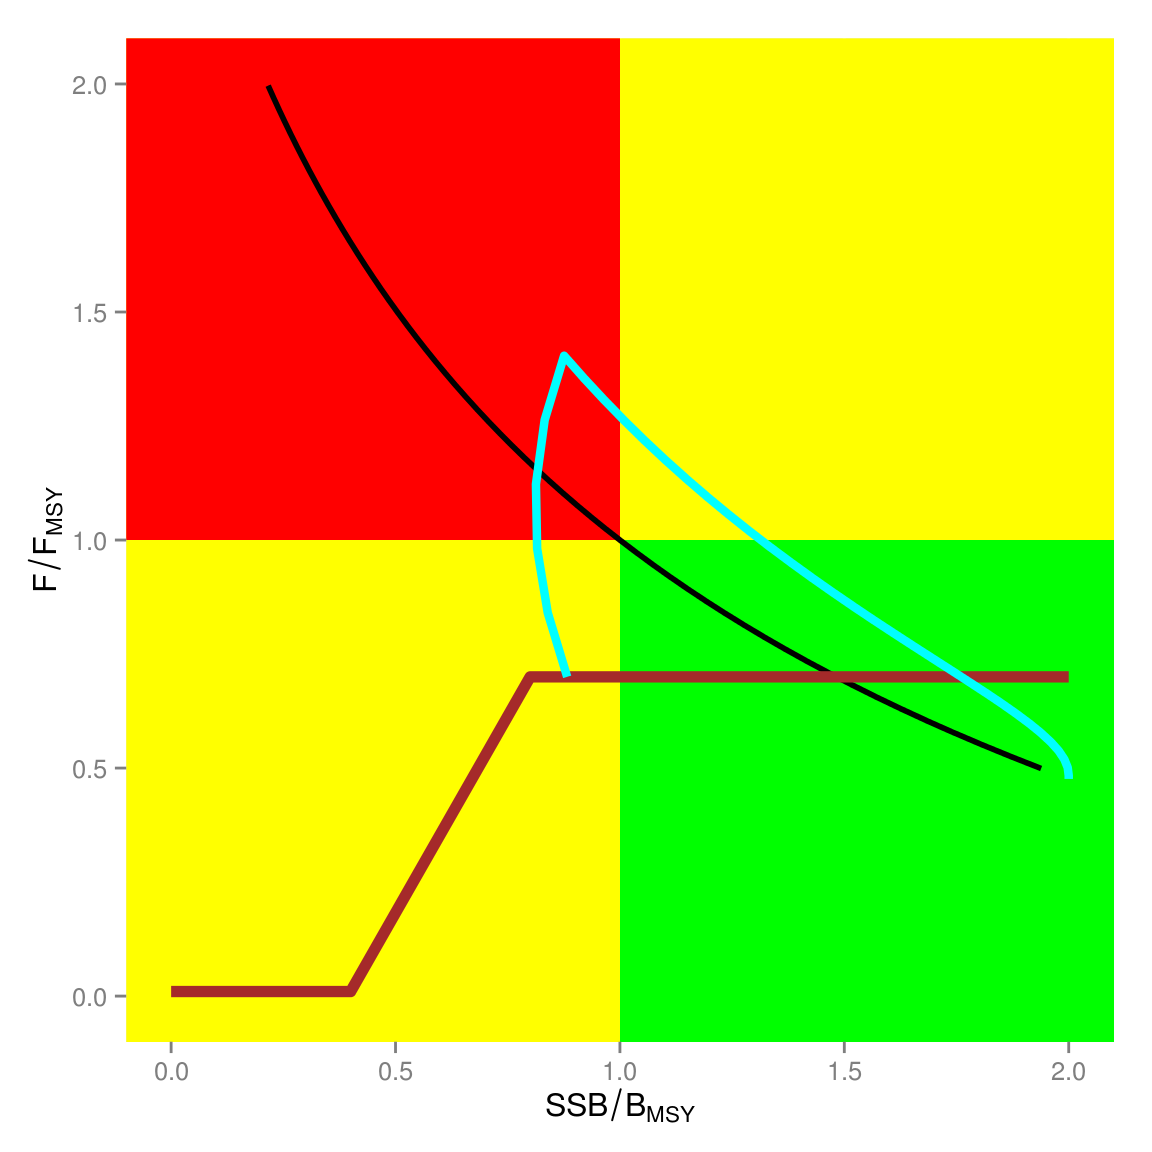
\includegraphics[width=6in]{hcr.png}
\label{fig:hcr}
\caption{Harvest Control Rule (brown) plotted on a phase plot of harvest rate relative to $F_{MSY}$ and stock biomass relative to $B_{MSY}$;
the light line is the simulated stock and the black line is the replacement line.}
\end{figure*}

%\begin{landscape}
\begin{figure*}[htbp]
\centering
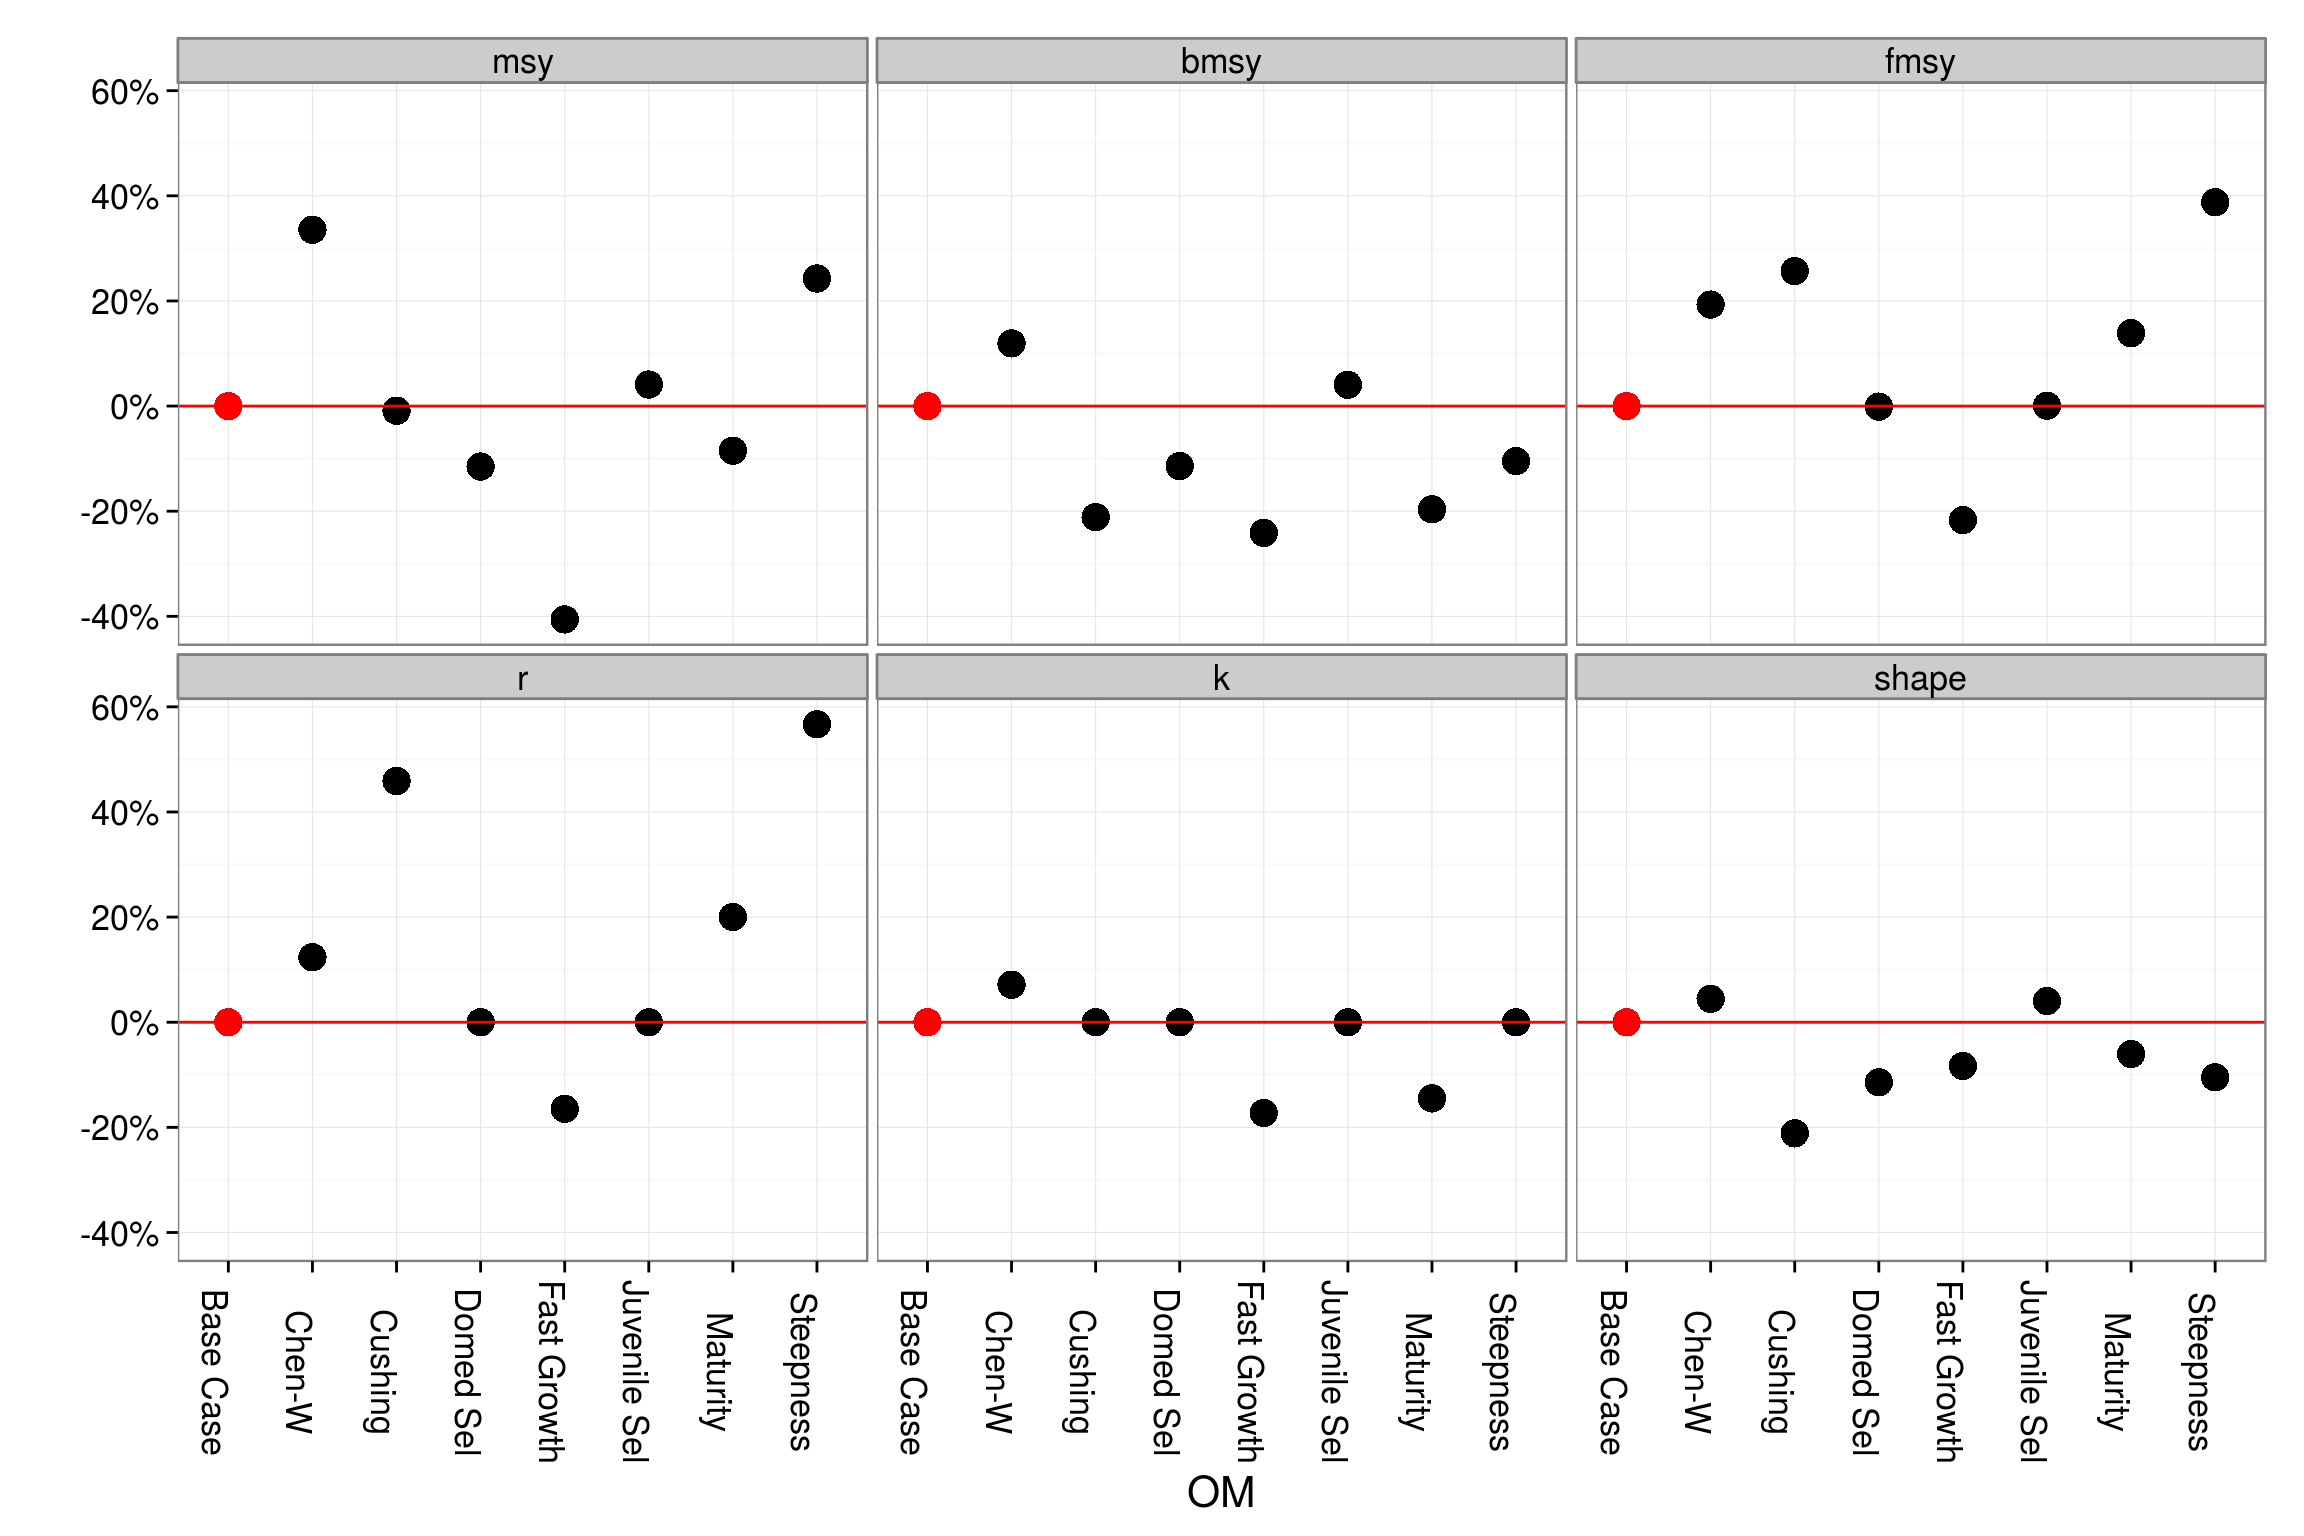
\includegraphics[width=6in]{ssOMs.png}
\caption{Population parameters and reference points by OM scenarios, values are relative to the Base Case (red).}
\label{fig:popPar}
\end{figure*}
%\end{landscape}

\begin{figure*}[htbp]
\centering
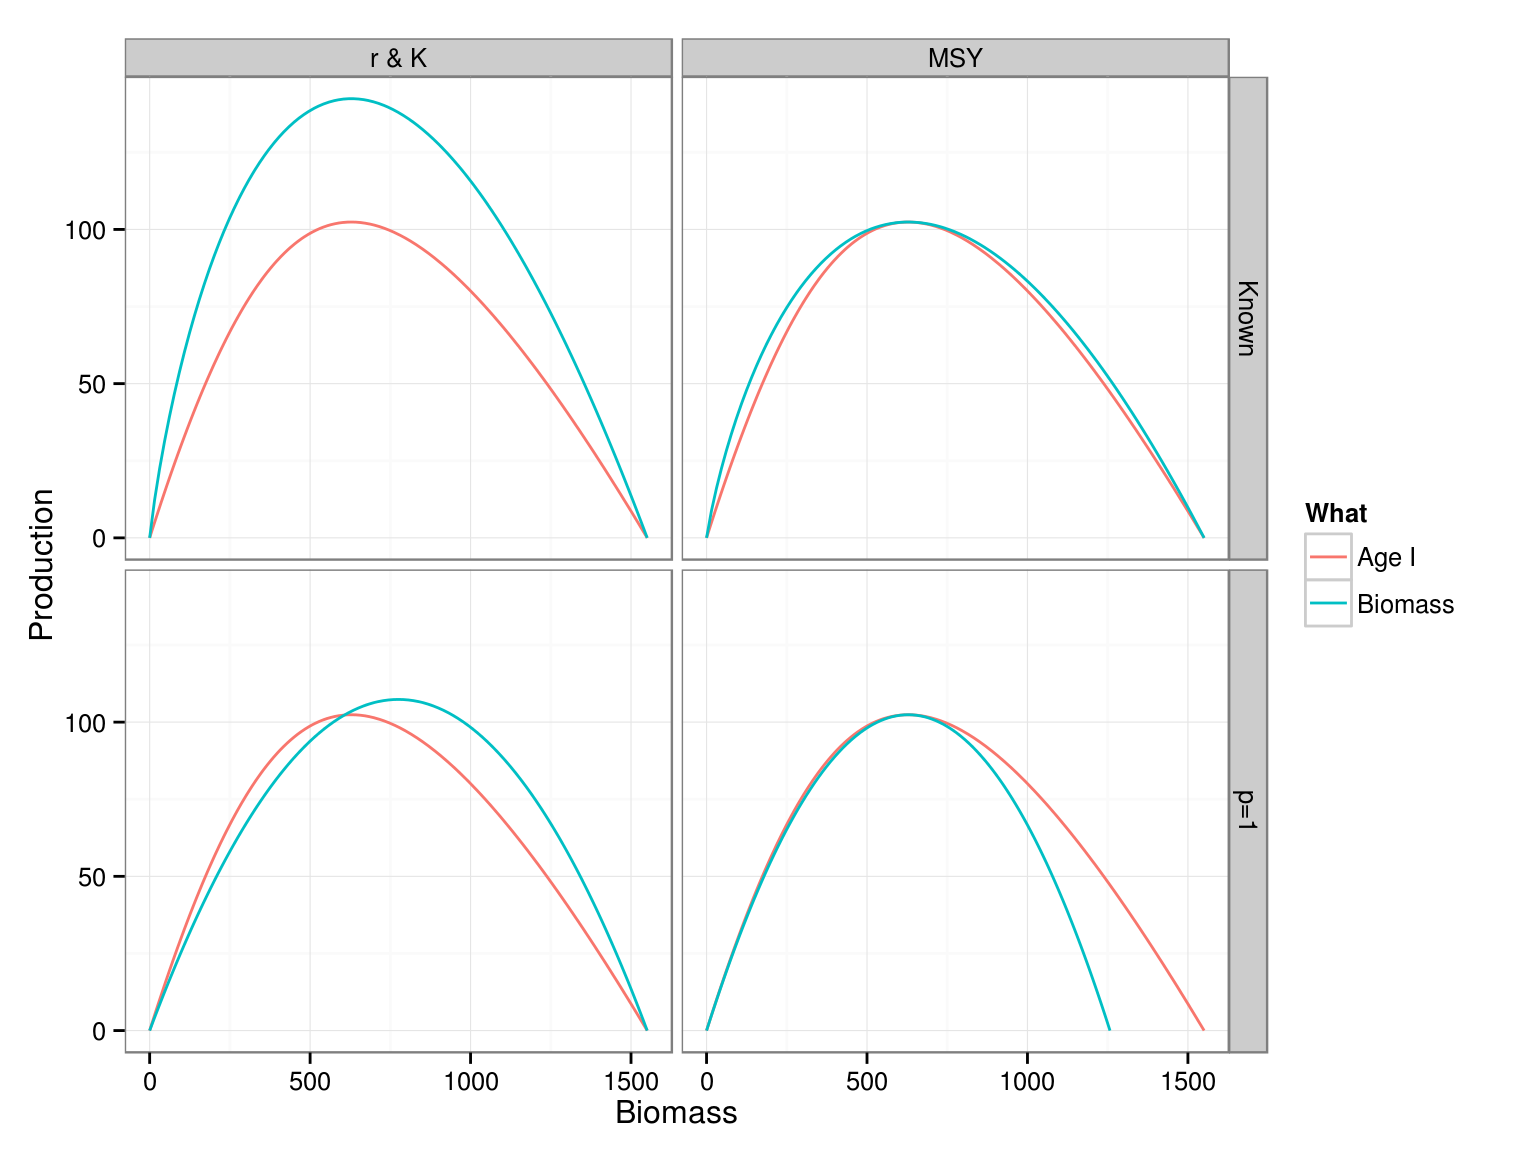
\includegraphics[width=6in]{pFn.png}
\caption{A comparison of age and biomass based production functions for the Base Case (i.e. for the OM and MP respectively). In all cases the age based production function is the same. The biomass based production function is calculated assuming, either that the function is symmetric (p=1) or the ratio of $B_{MSY}:K$ is the same as in the OM (known) and that either reference points or r\&K are the same as in the OM.}
\label{fig:pFn}
\end{figure*}

\begin{figure*}[htbp]
\centering
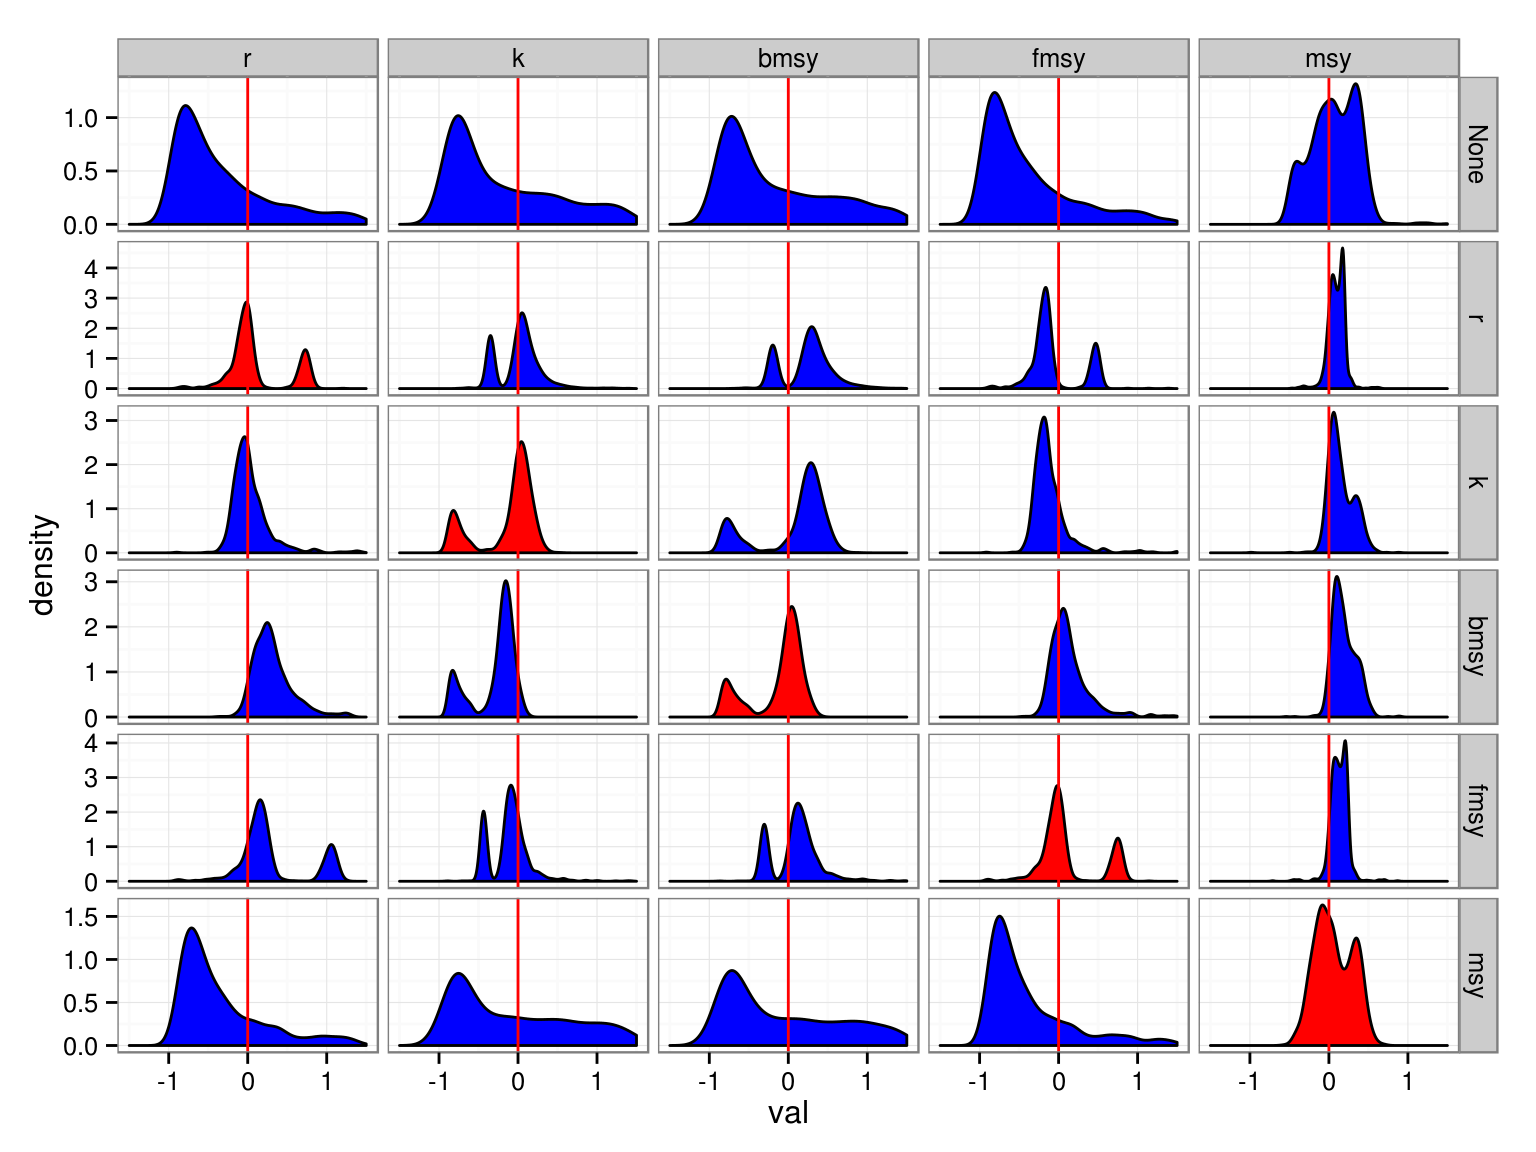
\includegraphics[width=6in]{SA1.png}
\caption{A comparison of reference points and population parameters estimated by the Stock Assessment in the MP for the Base Case OM, where the production function is assumed to be symmetric (p=1). Columns give the quantity and rows indicate the value was penalised in the likelihood based on the OM value.}
\label{fig:sa1}
\end{figure*}

\begin{figure*}[htbp]
\centering
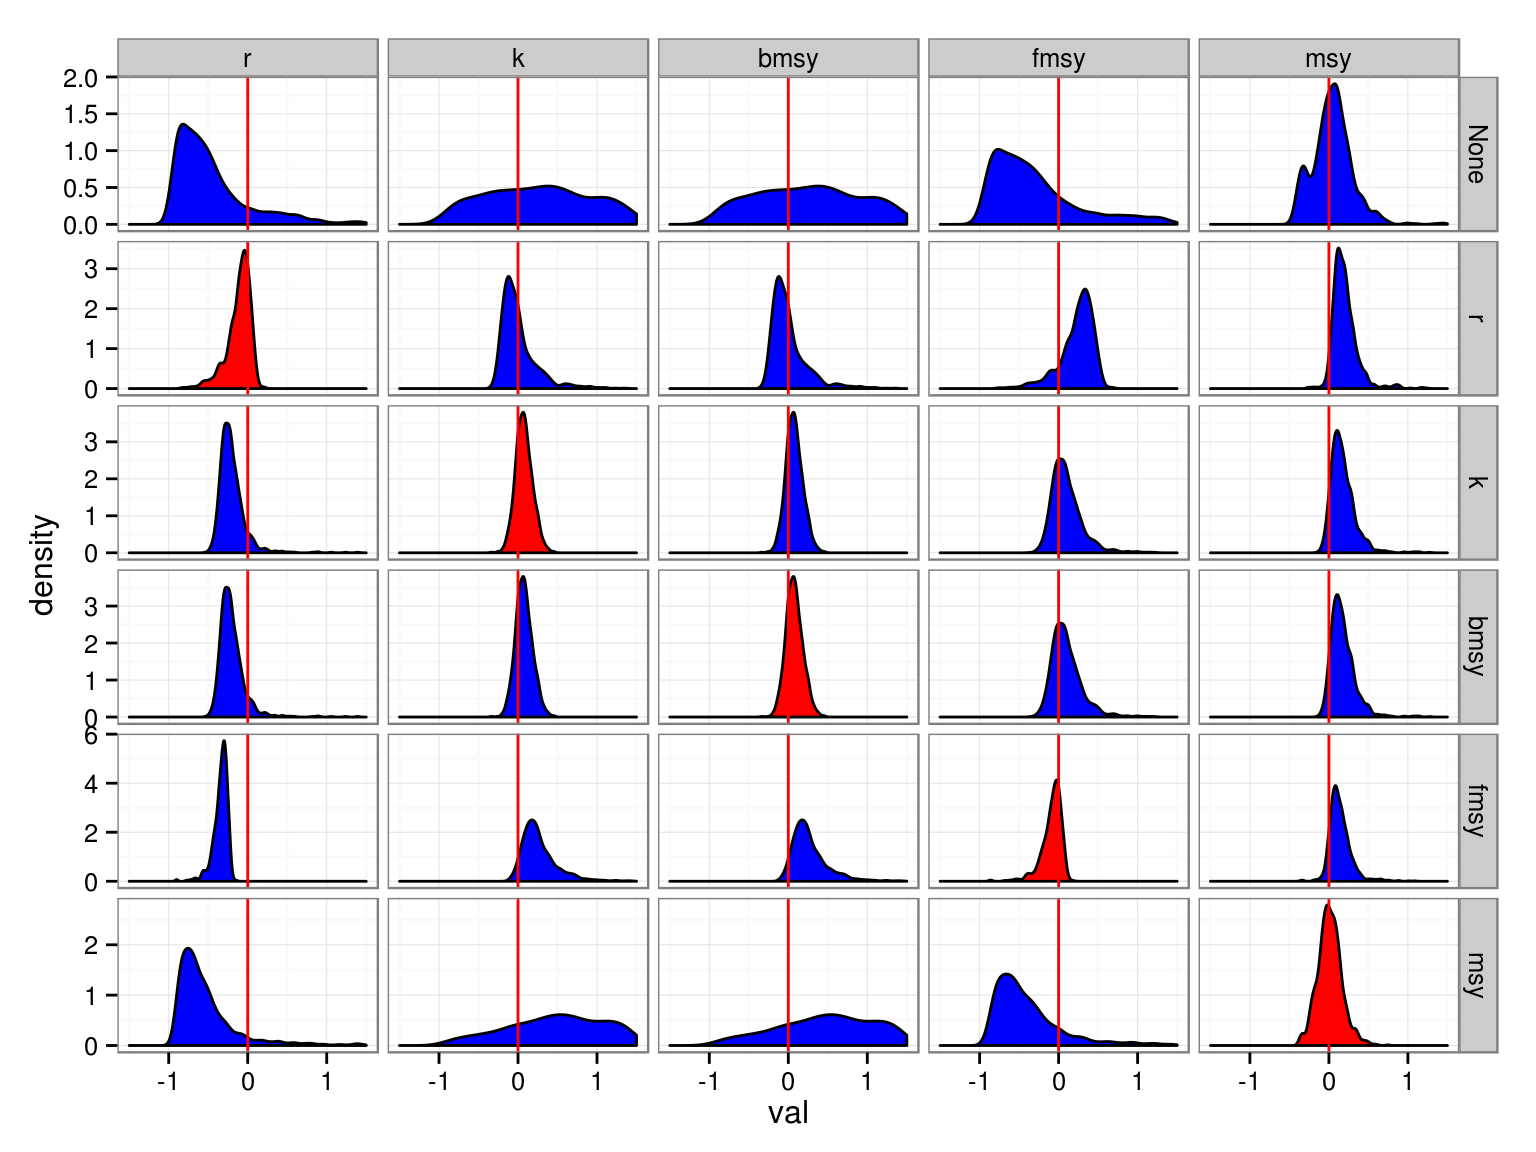
\includegraphics[width=6in]{SA2.png}
\caption{A comparison of reference points and population parameters estimated by the Stock Assessment in the MP for the Base Case OM, where the production function has the same shape as in the OM. Columns give the quantity and rows indicate the value was penalised in the likelihood based on the OM value.}
\label{fig:sa2}
\end{figure*}


\begin{figure*}[htbp]
\centering
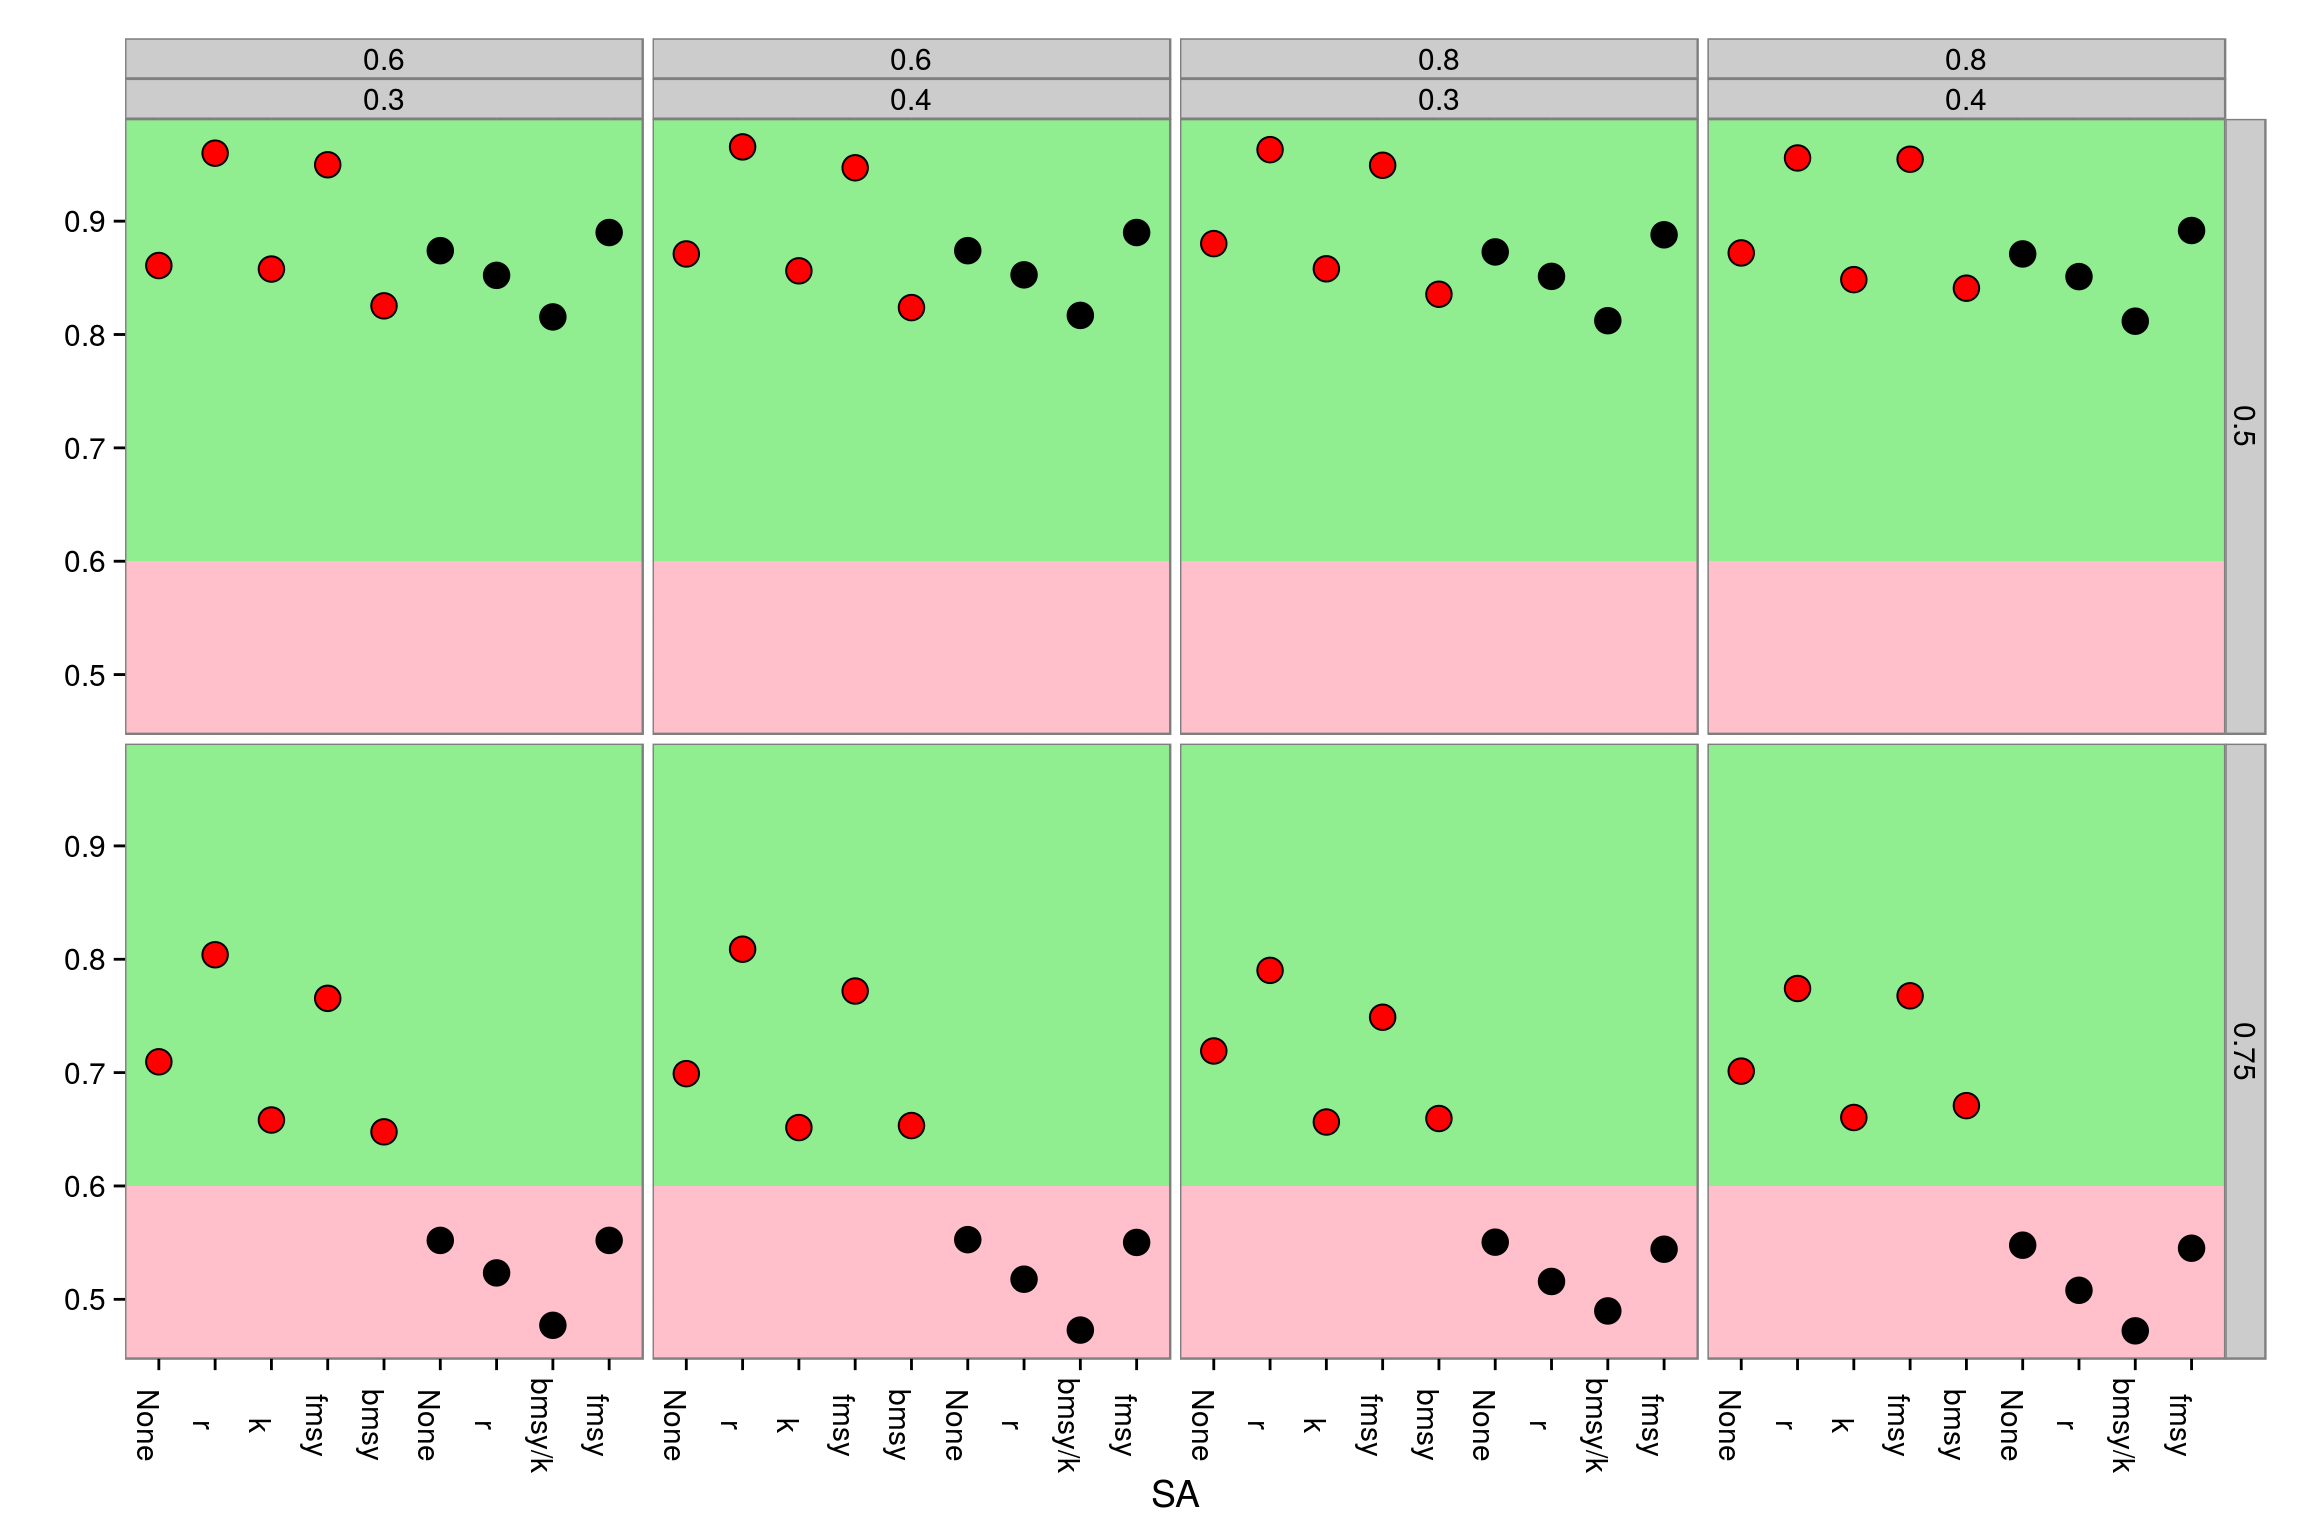
\includegraphics[width=6in]{ssGreen.png}
\caption{Probability of being in the green quadrant of the Kobe phase plot, by biomass thresholds and limits as a proportion of $B_{MSY}$ (columns) and fishing mortality targets as a proportion of $F_{MSY}$(rows)}
\label{fig:ssGreen}
\end{figure*}

\begin{figure*}[htbp]
\centering
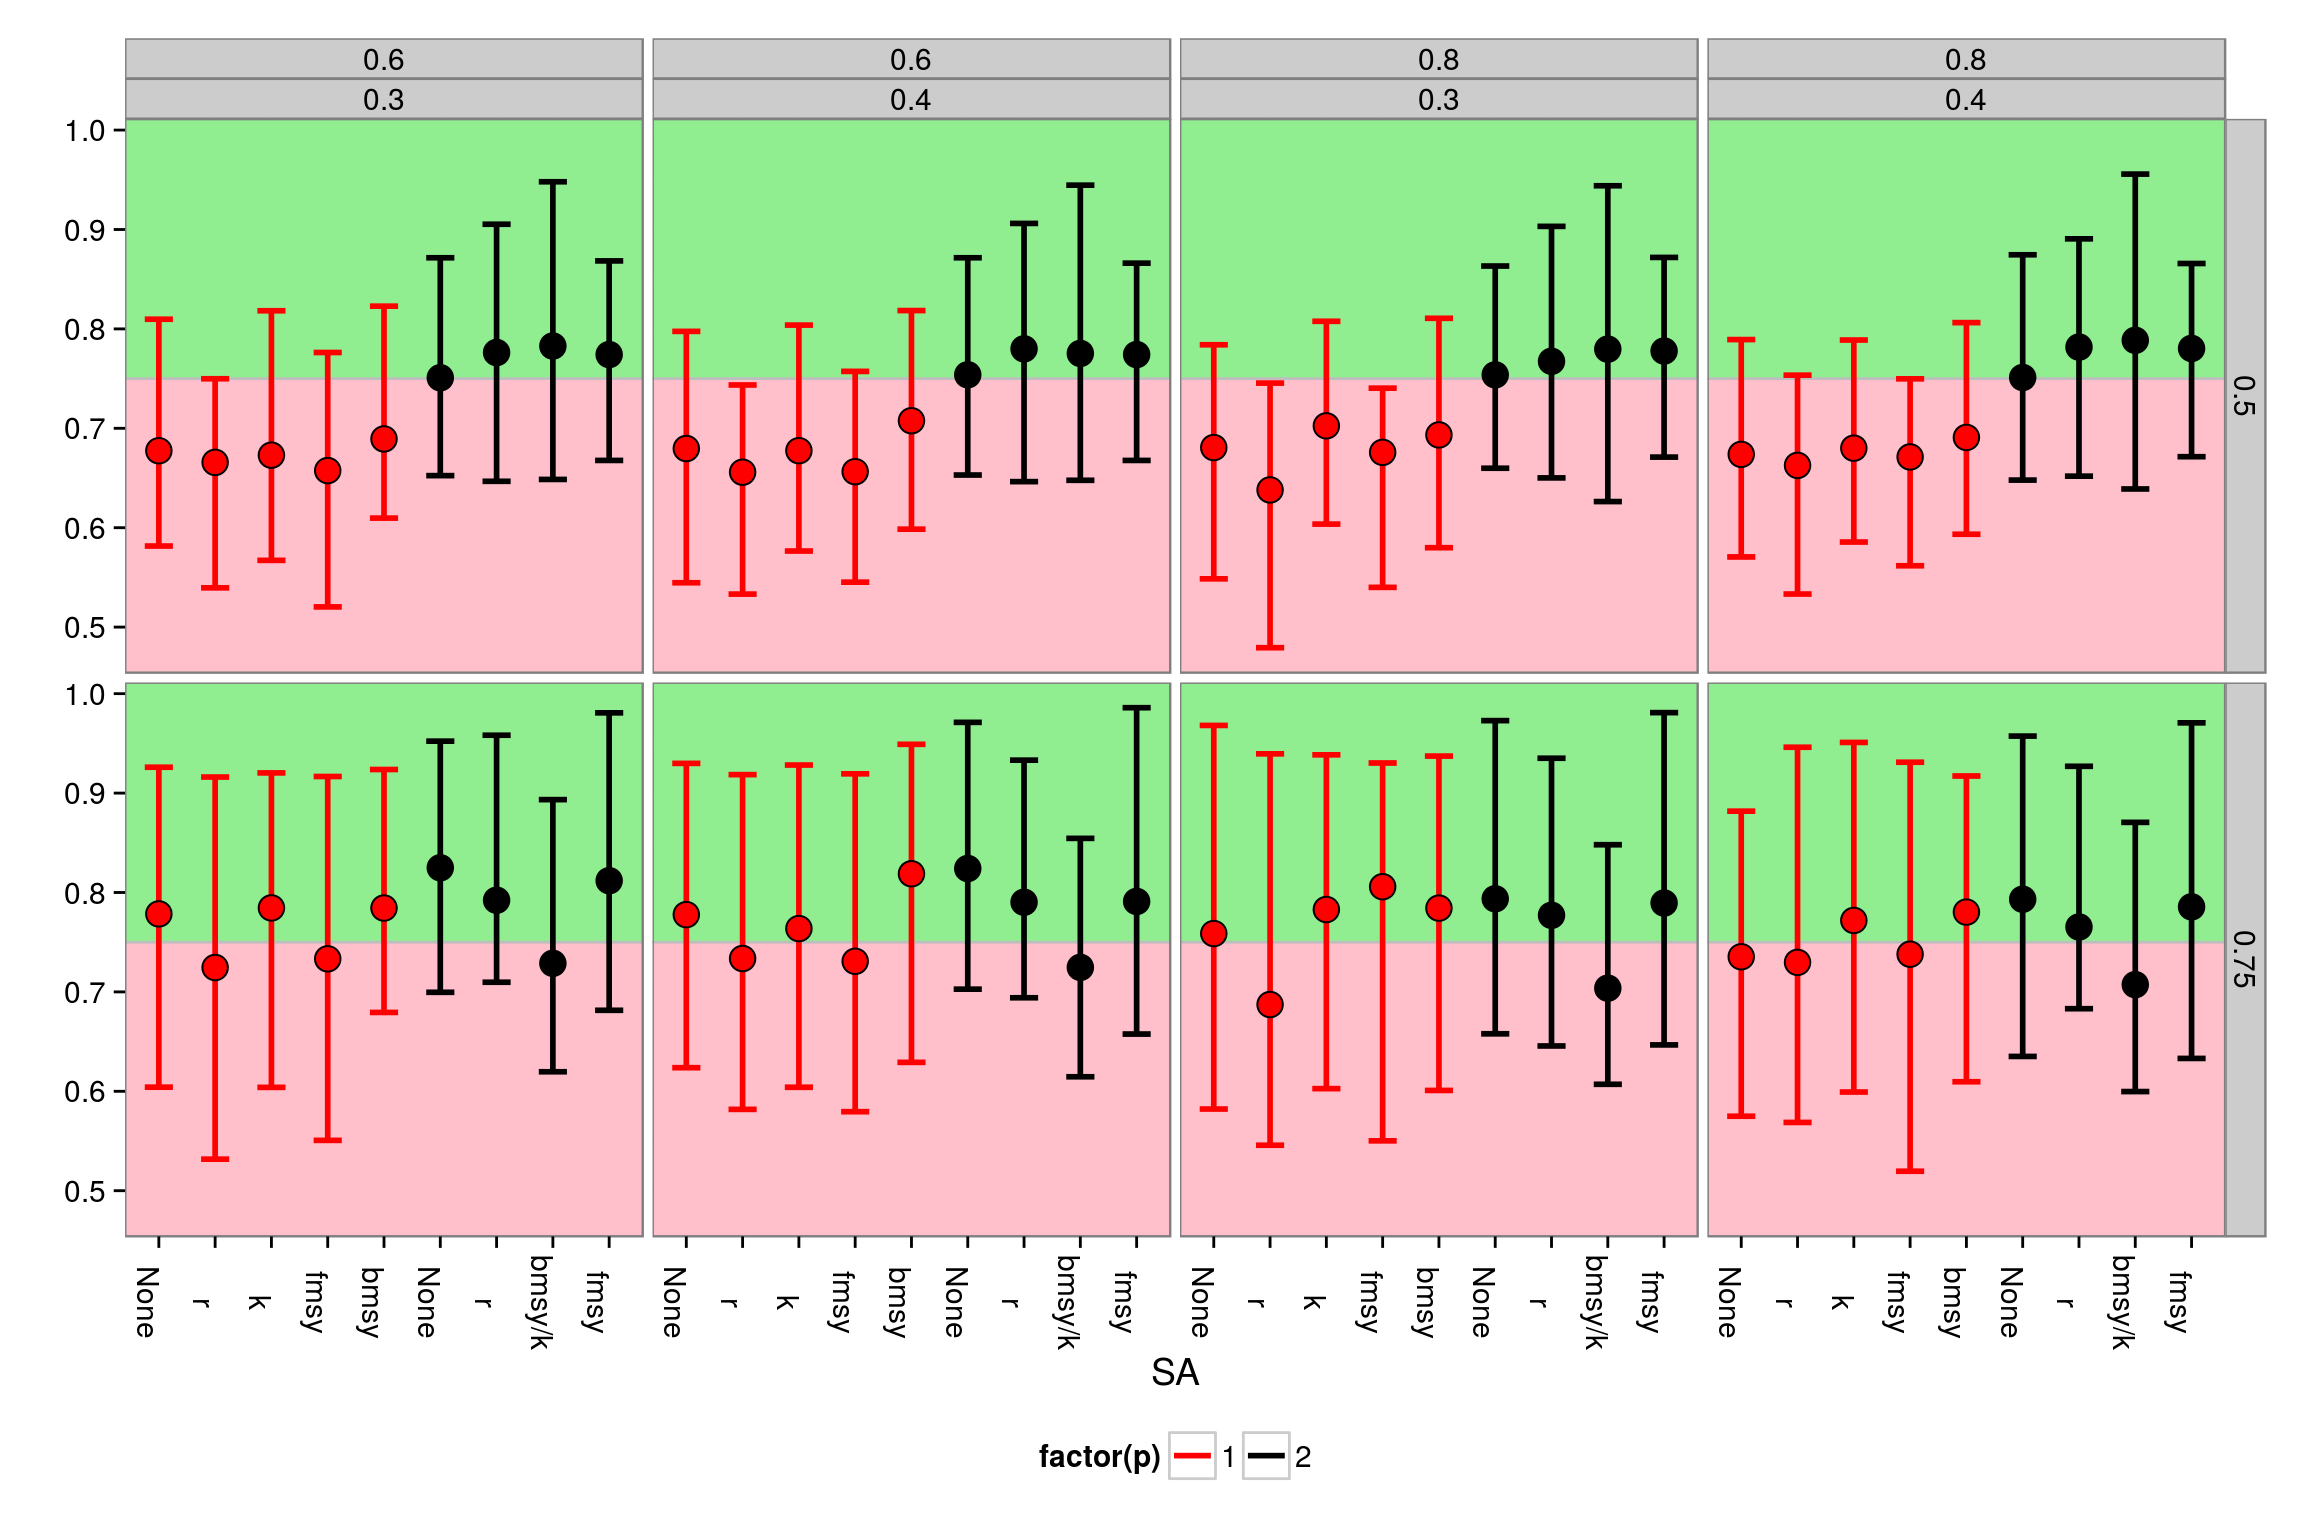
\includegraphics[width=6in]{ssY.png}
\caption{Yield relative to MSY, interquartile range and medians by biomass thresholds and limits as a proportion of $B_{MSY}$ (columns) and fishing mortality targets as a proportion of $F_{MSY}$(rows)}
\label{fig:ssY}
\end{figure*}

%\begin{tabular}{c}
  %\num\putindeepbox[7pt]{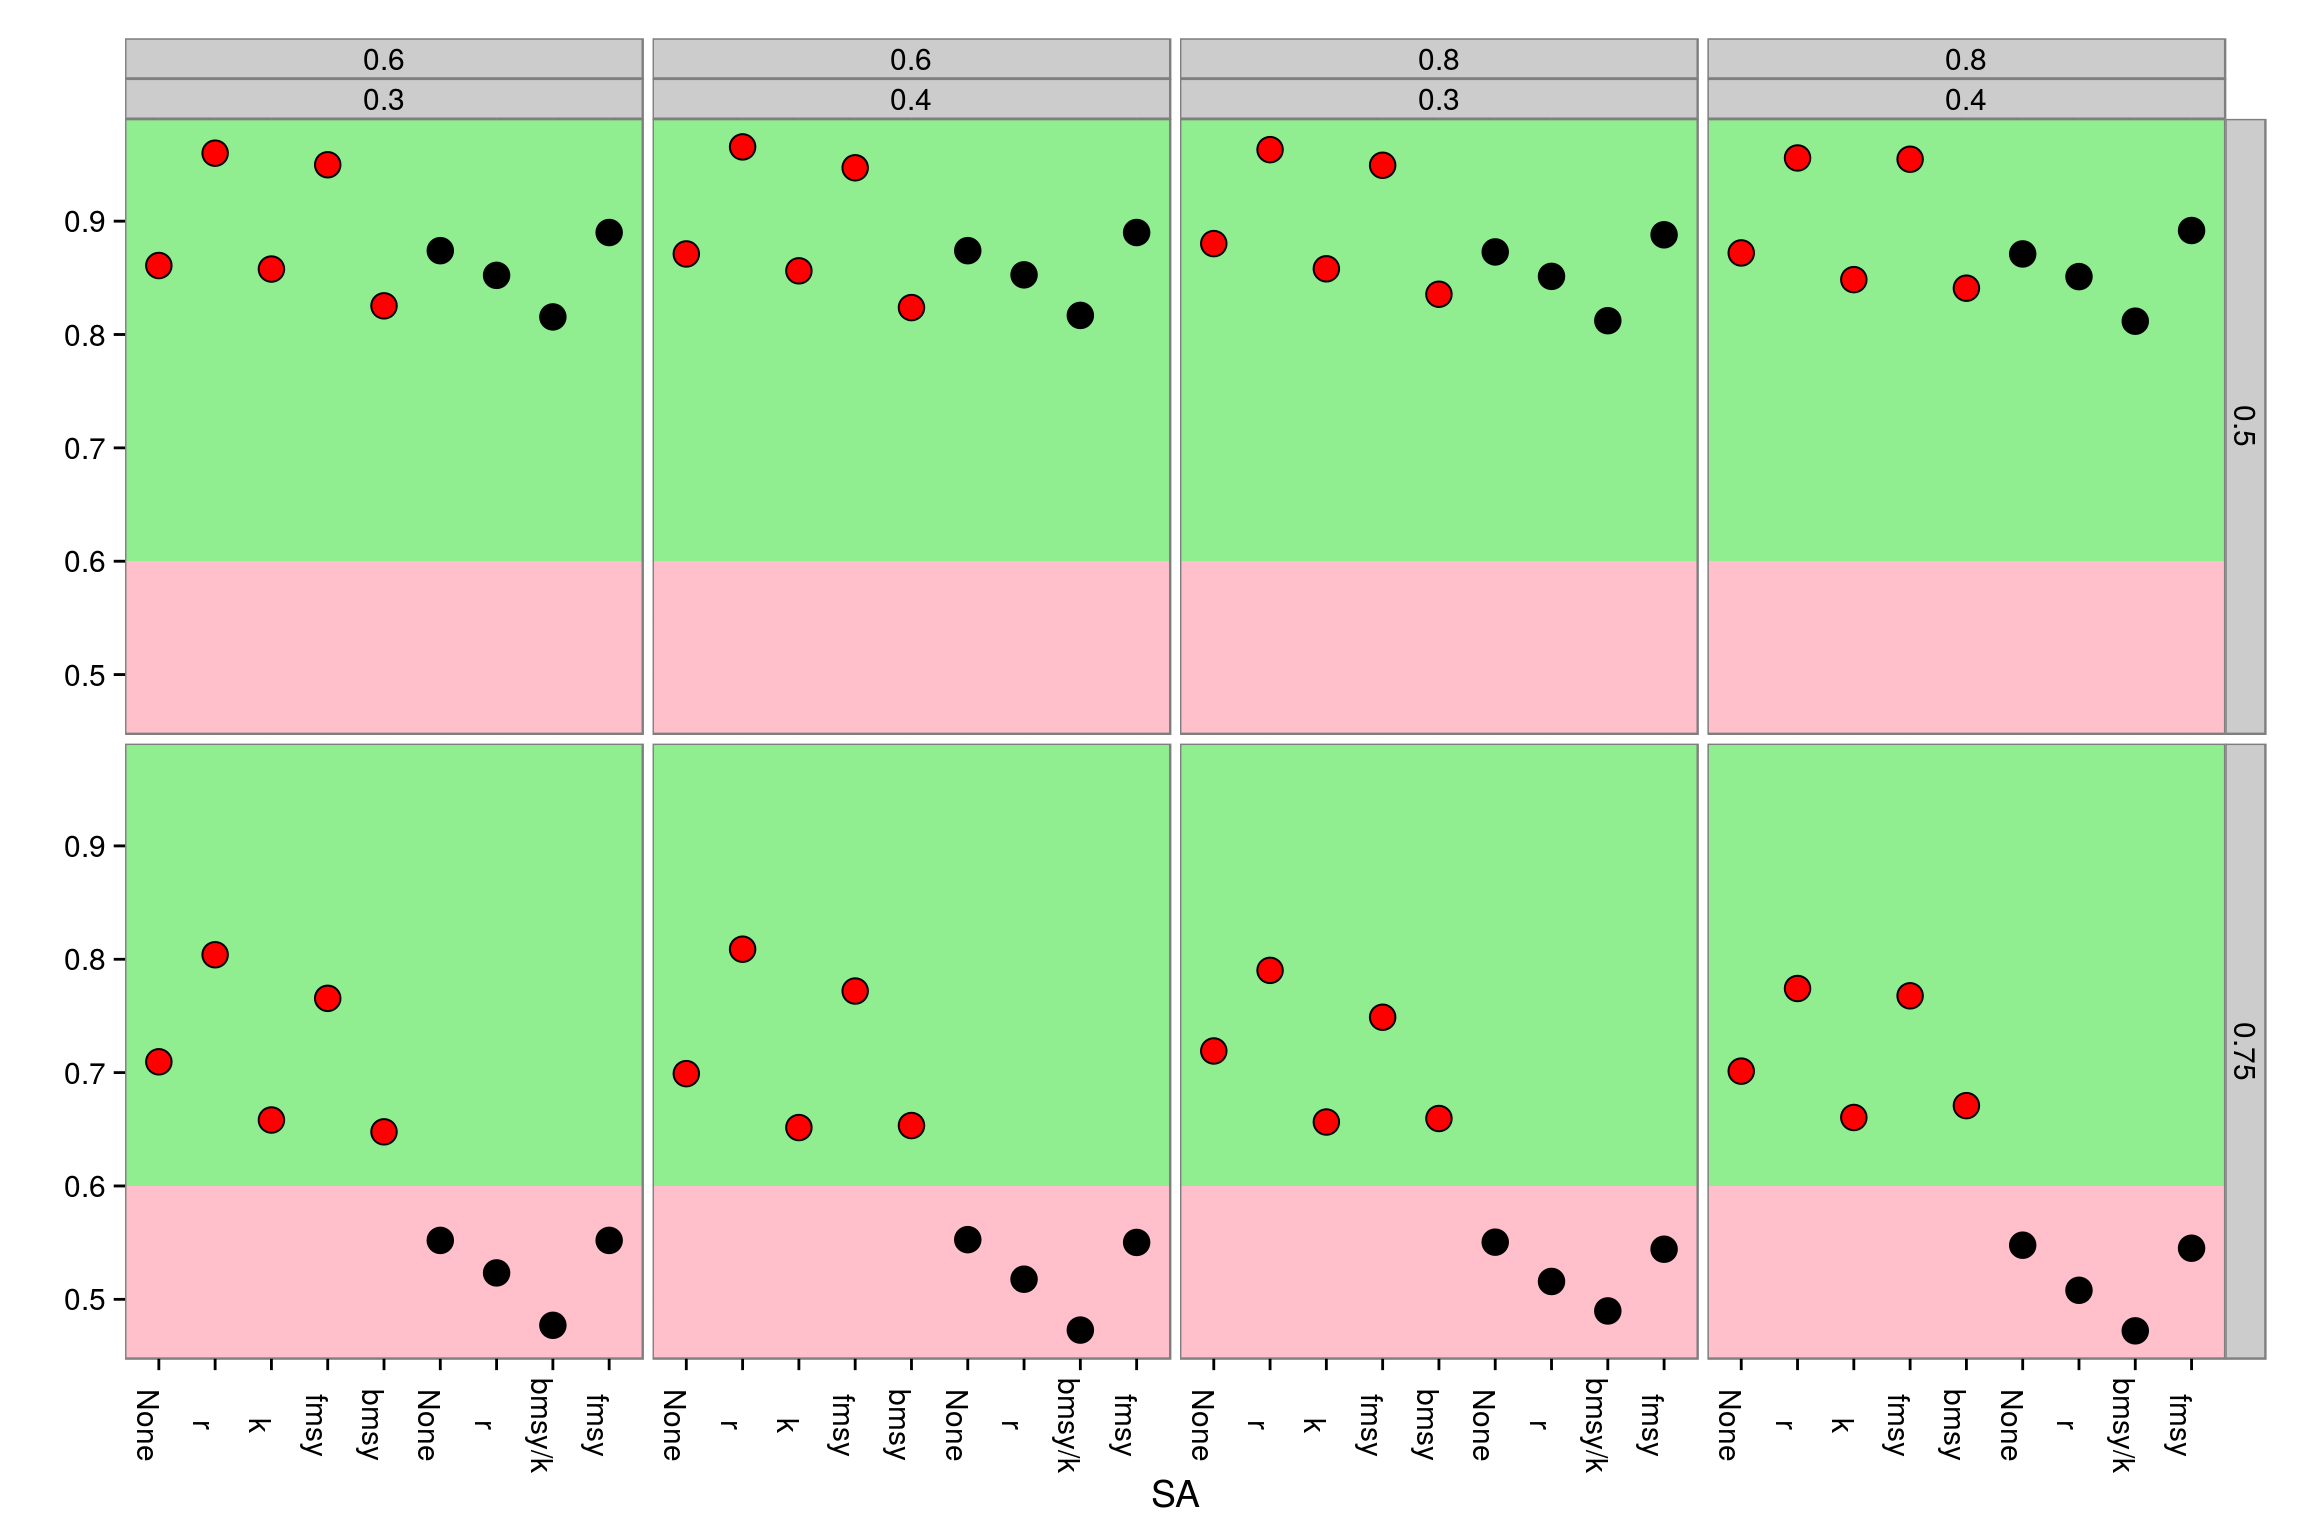
\includegraphics[width=7.2in]{ssGreen.png}}\\
  %\num\putindeepbox[7pt]{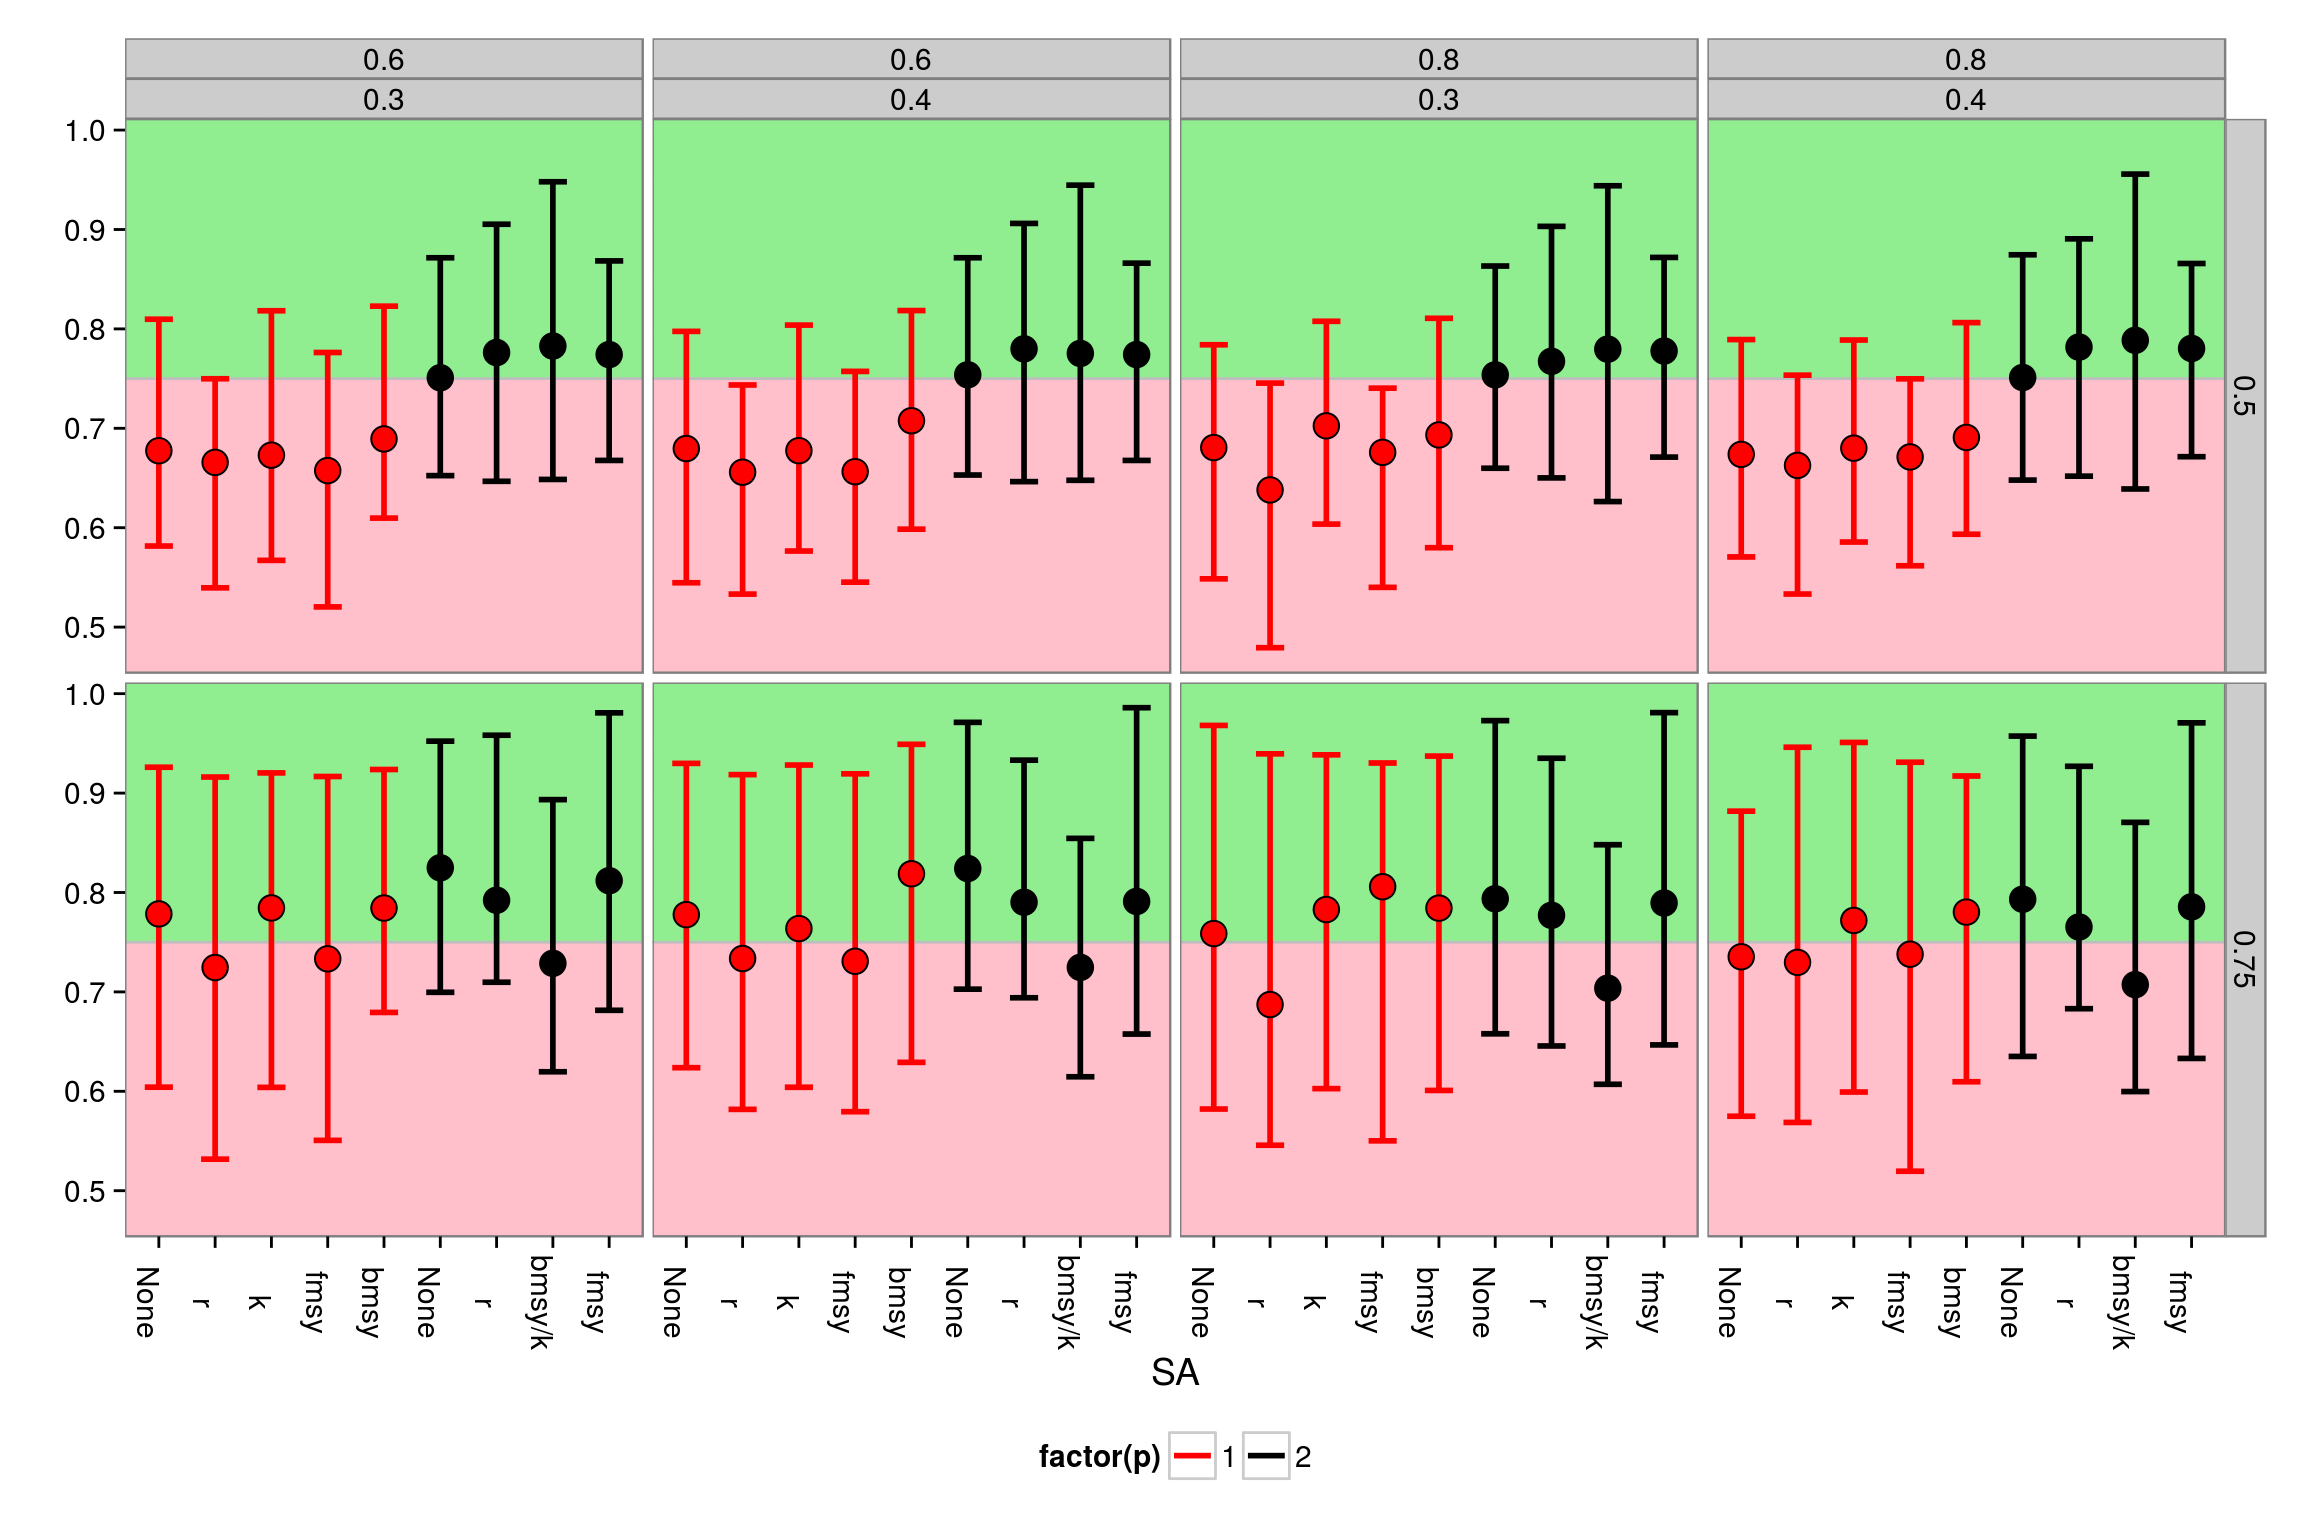
\includegraphics[width=7.2in]{ssY.png}} \\
%\label{fig:phase1}
%\end{tabular}


%\begin{landscape}
\begin{figure*}[htbp]
\centering
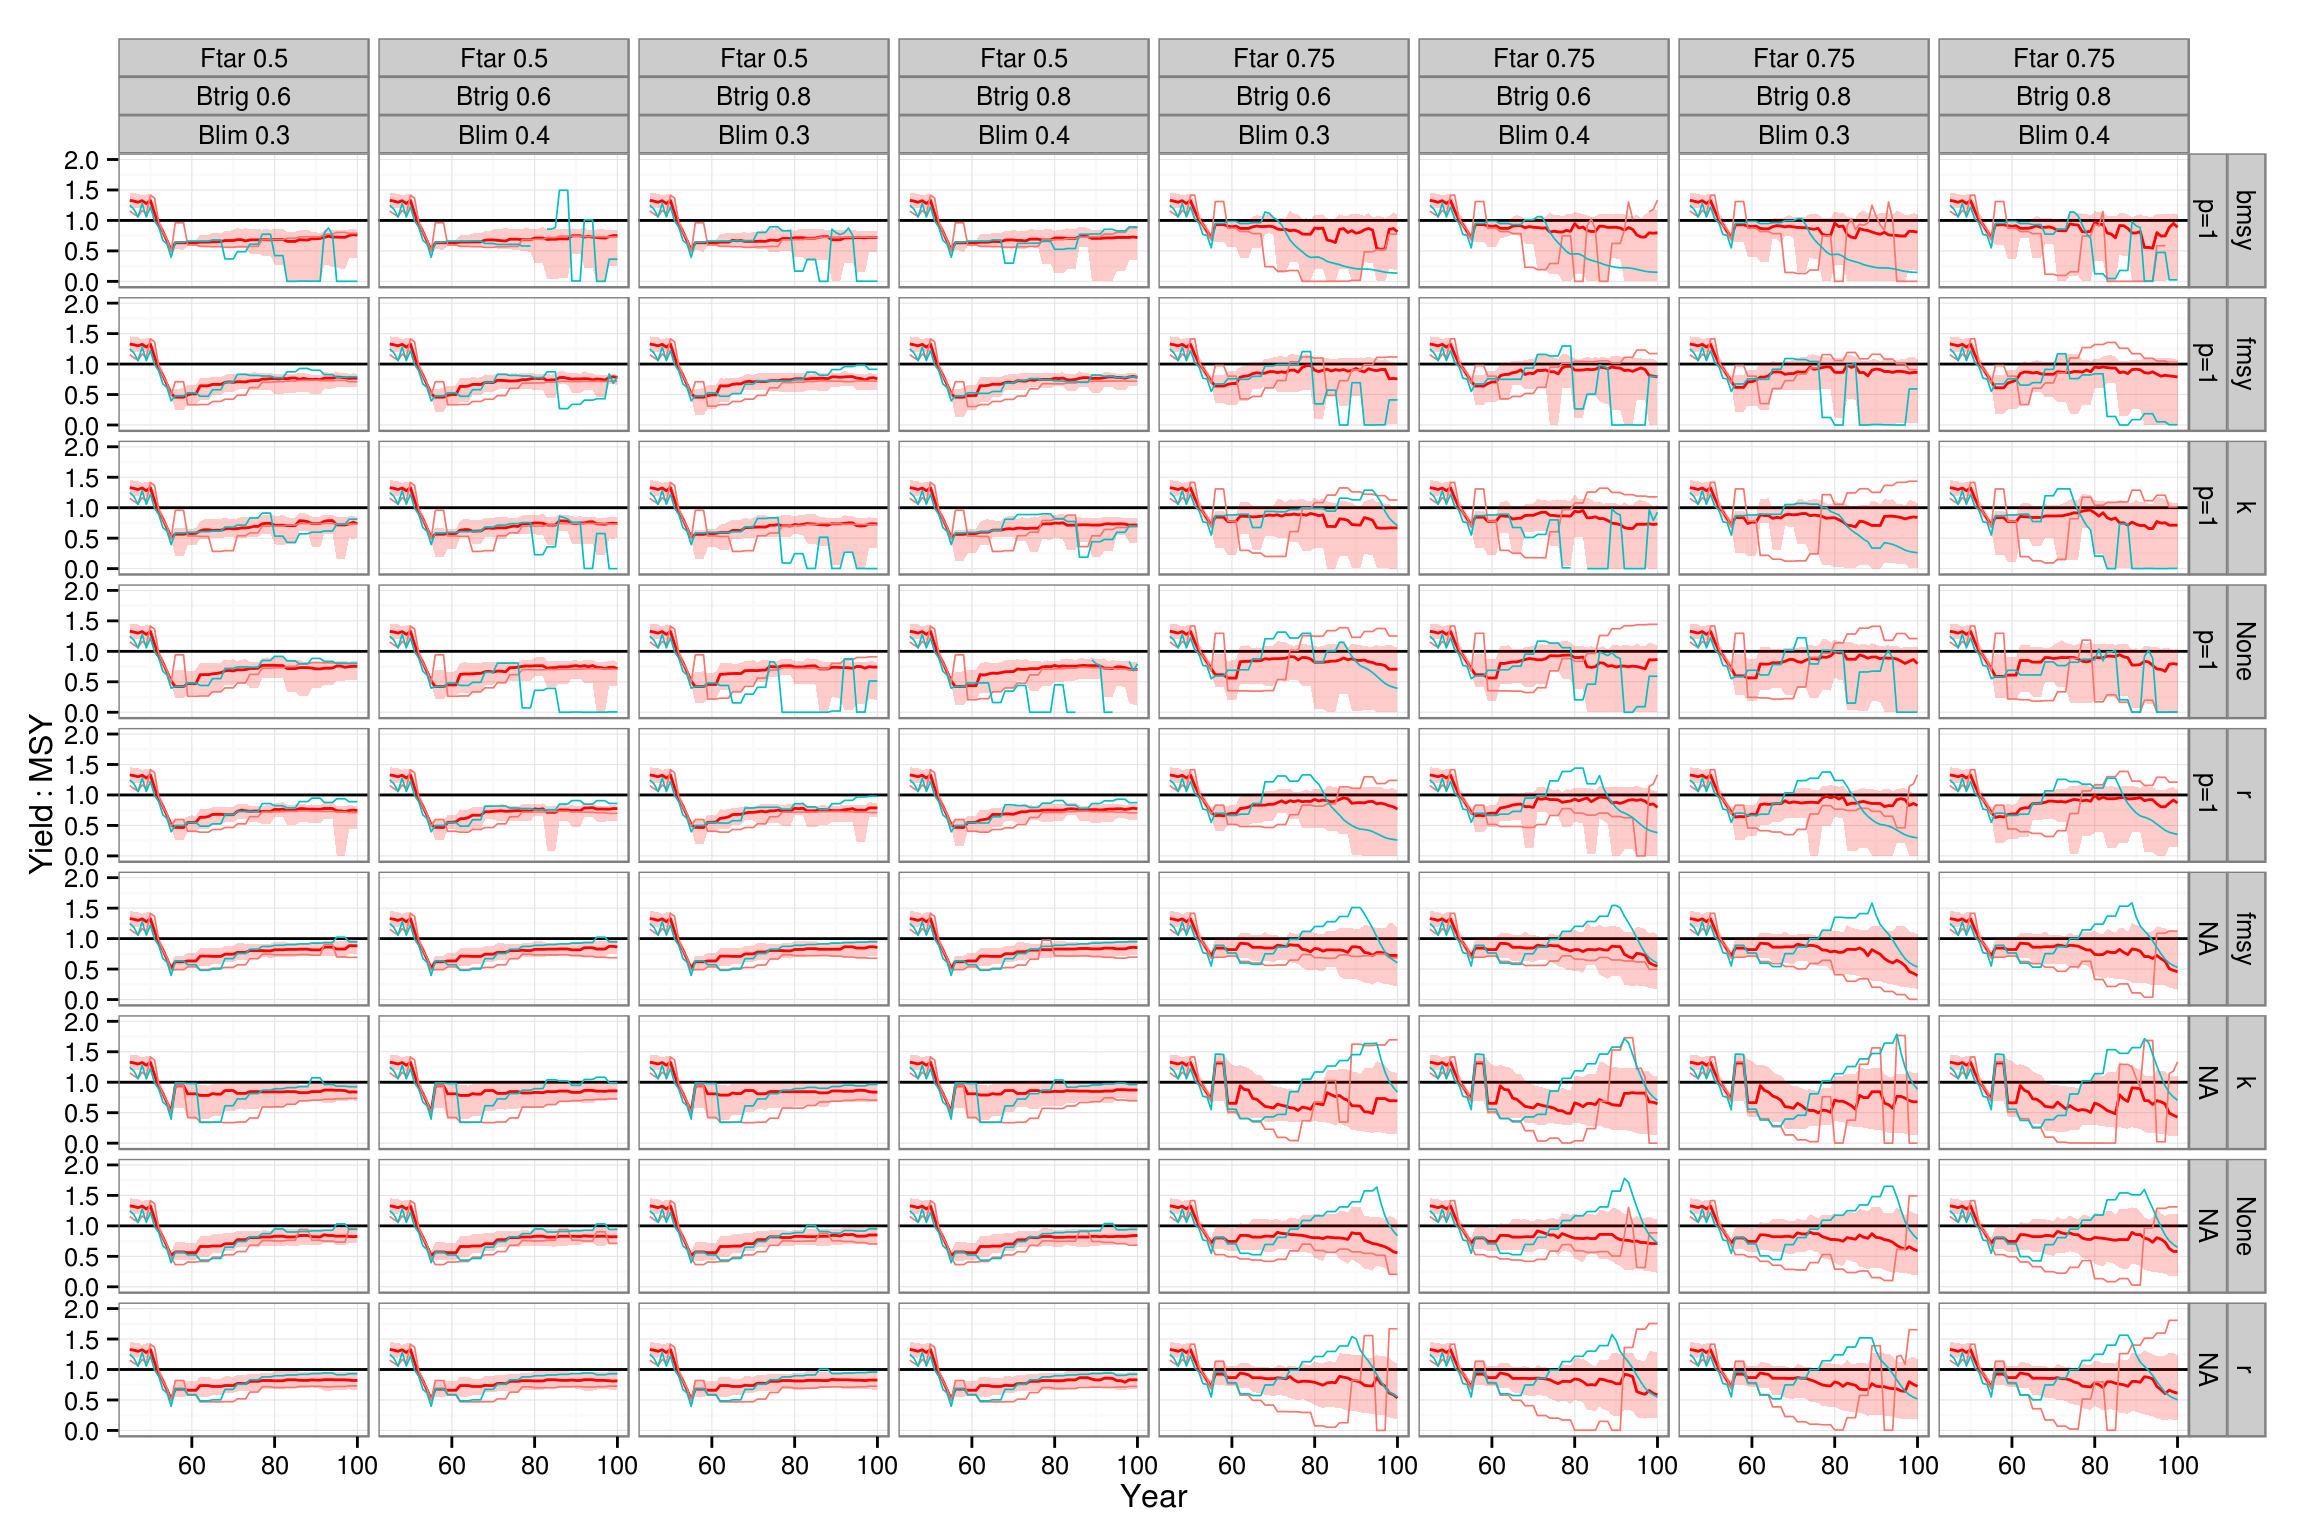
\includegraphics[width=6in]{tscatch.png}
\caption{Time series of $Catch:MSY$ by HCR (column) and stock assessment options (row). The shaded area represent the interquartile range with the median (thick line) and the thin lines two example Monte Carlo runs.}
\label{fig:tscatch}
\end{figure*}
%\end{landscape}

%\begin{landscape}
\begin{figure*}[htbp]
\centering
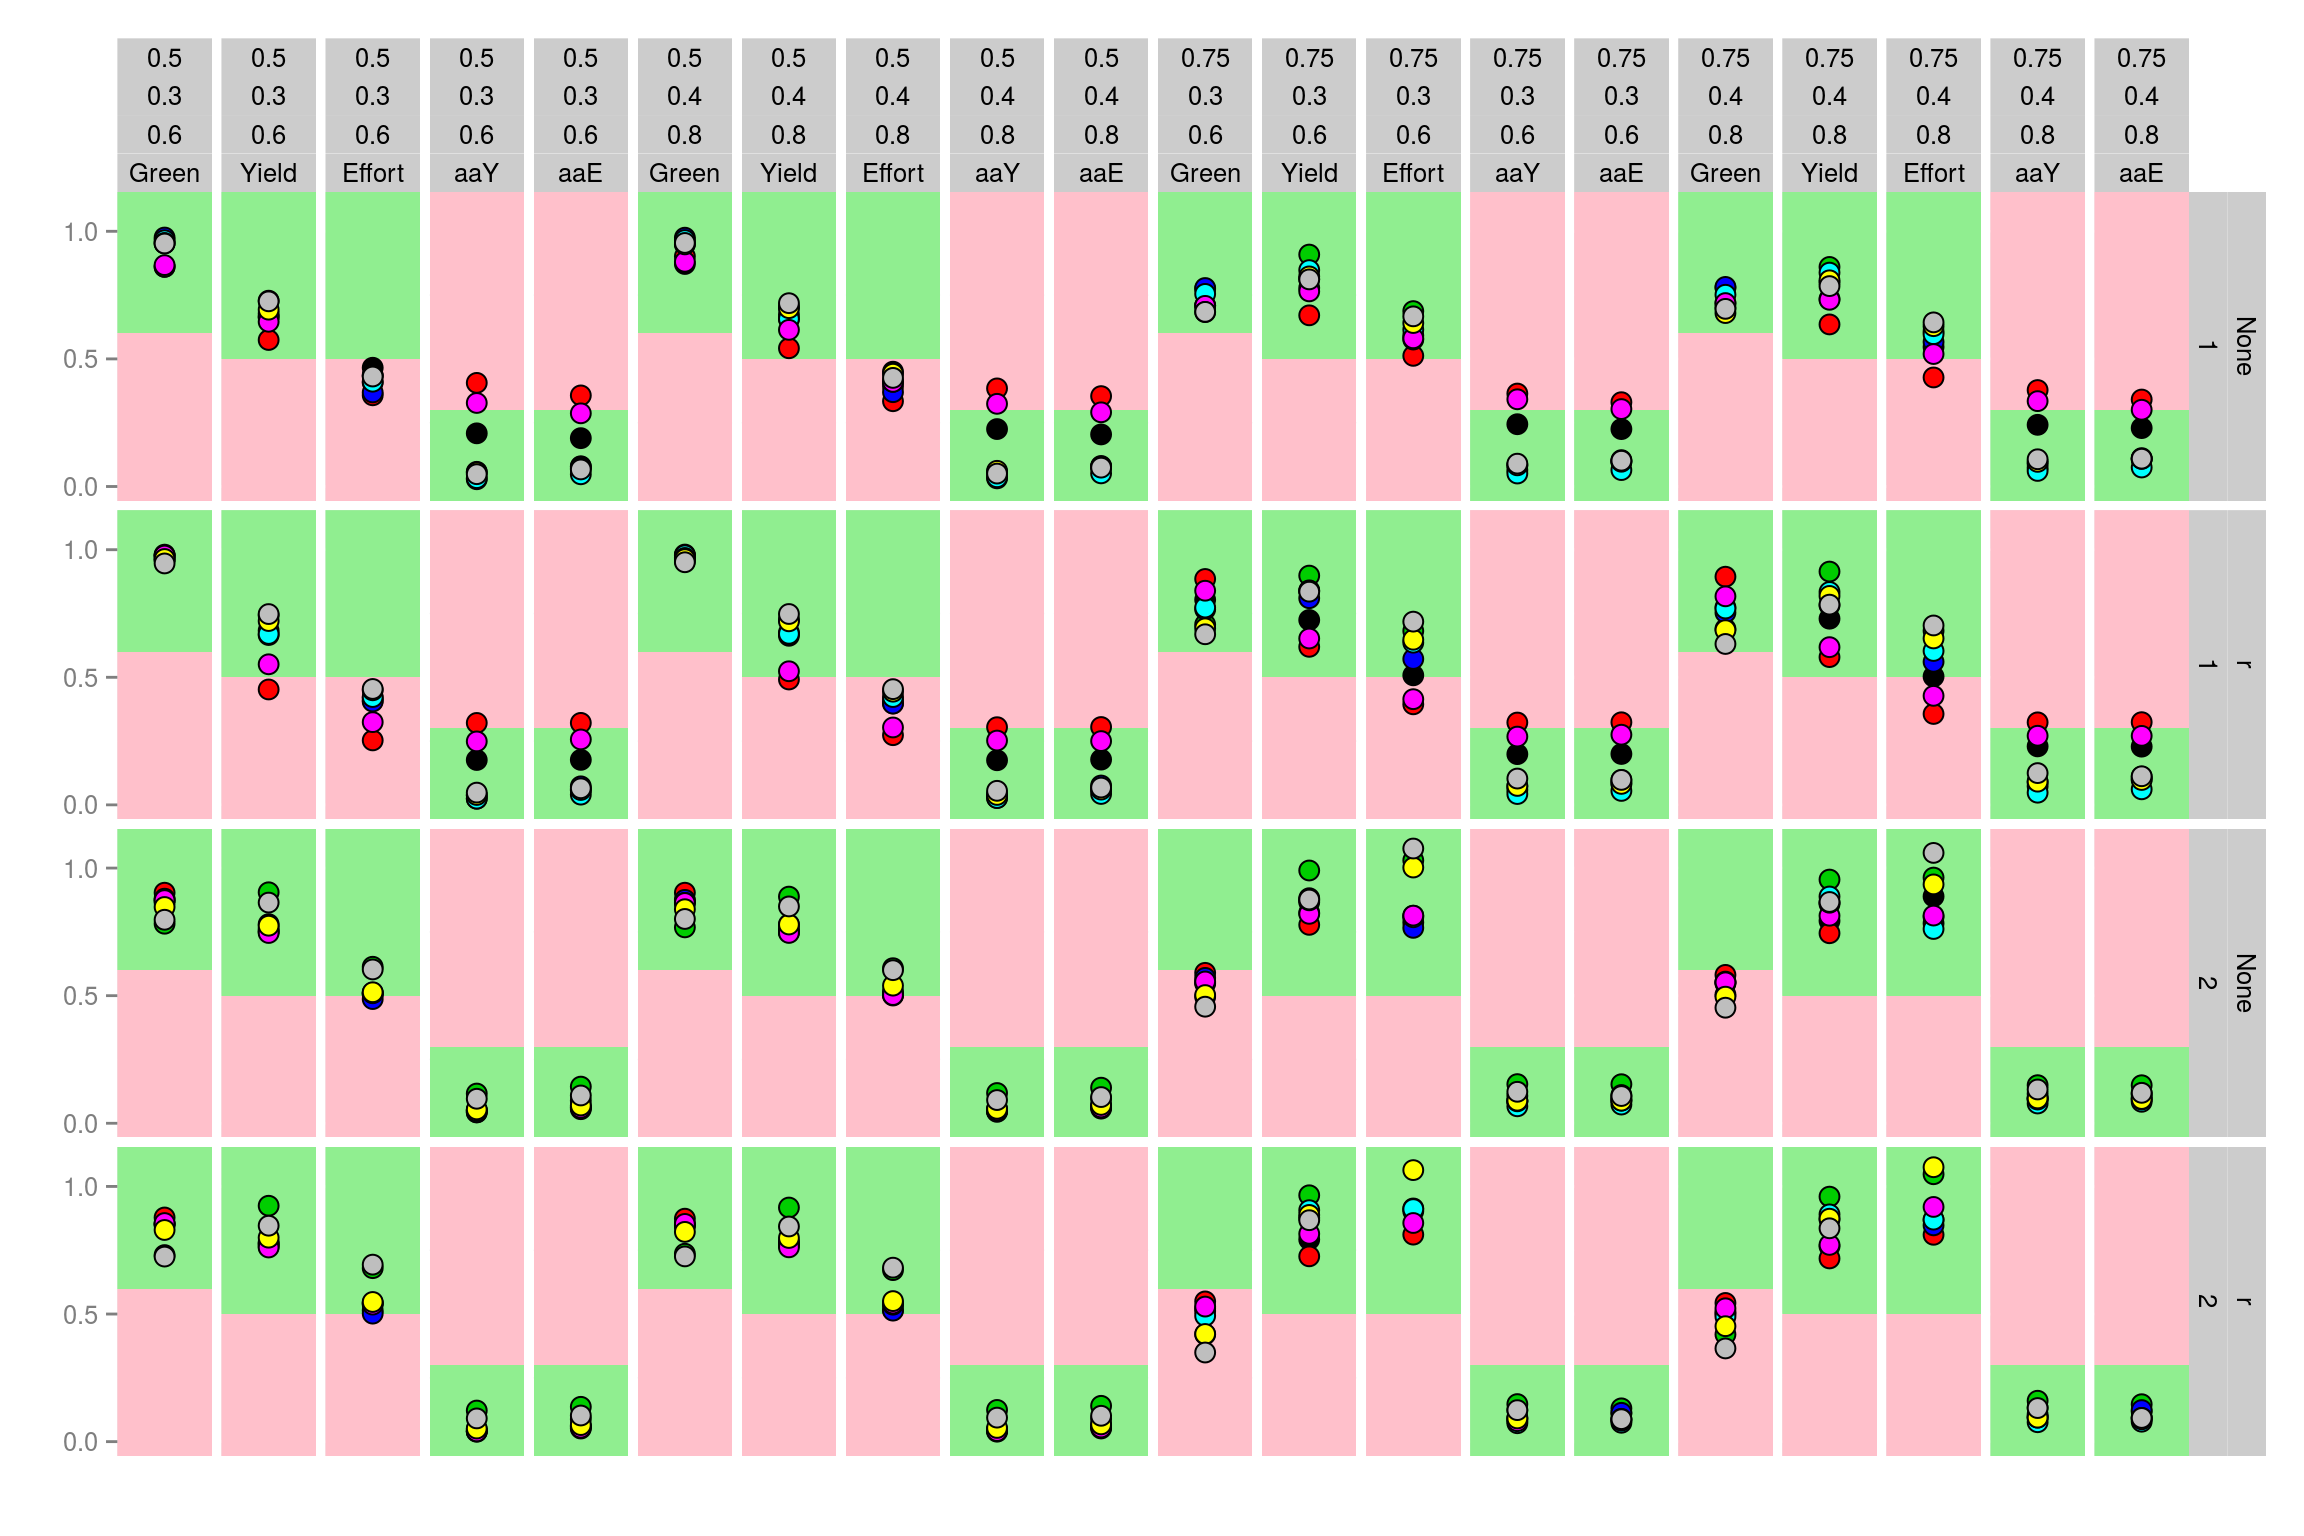
\includegraphics[width=6in]{ssSmry.png}
\caption{Summary.}
\label{fig:smry}
\end{figure*}
%\end{landscape}



%\begin{landscape}
\begin{figure*}[htbp]
\centering
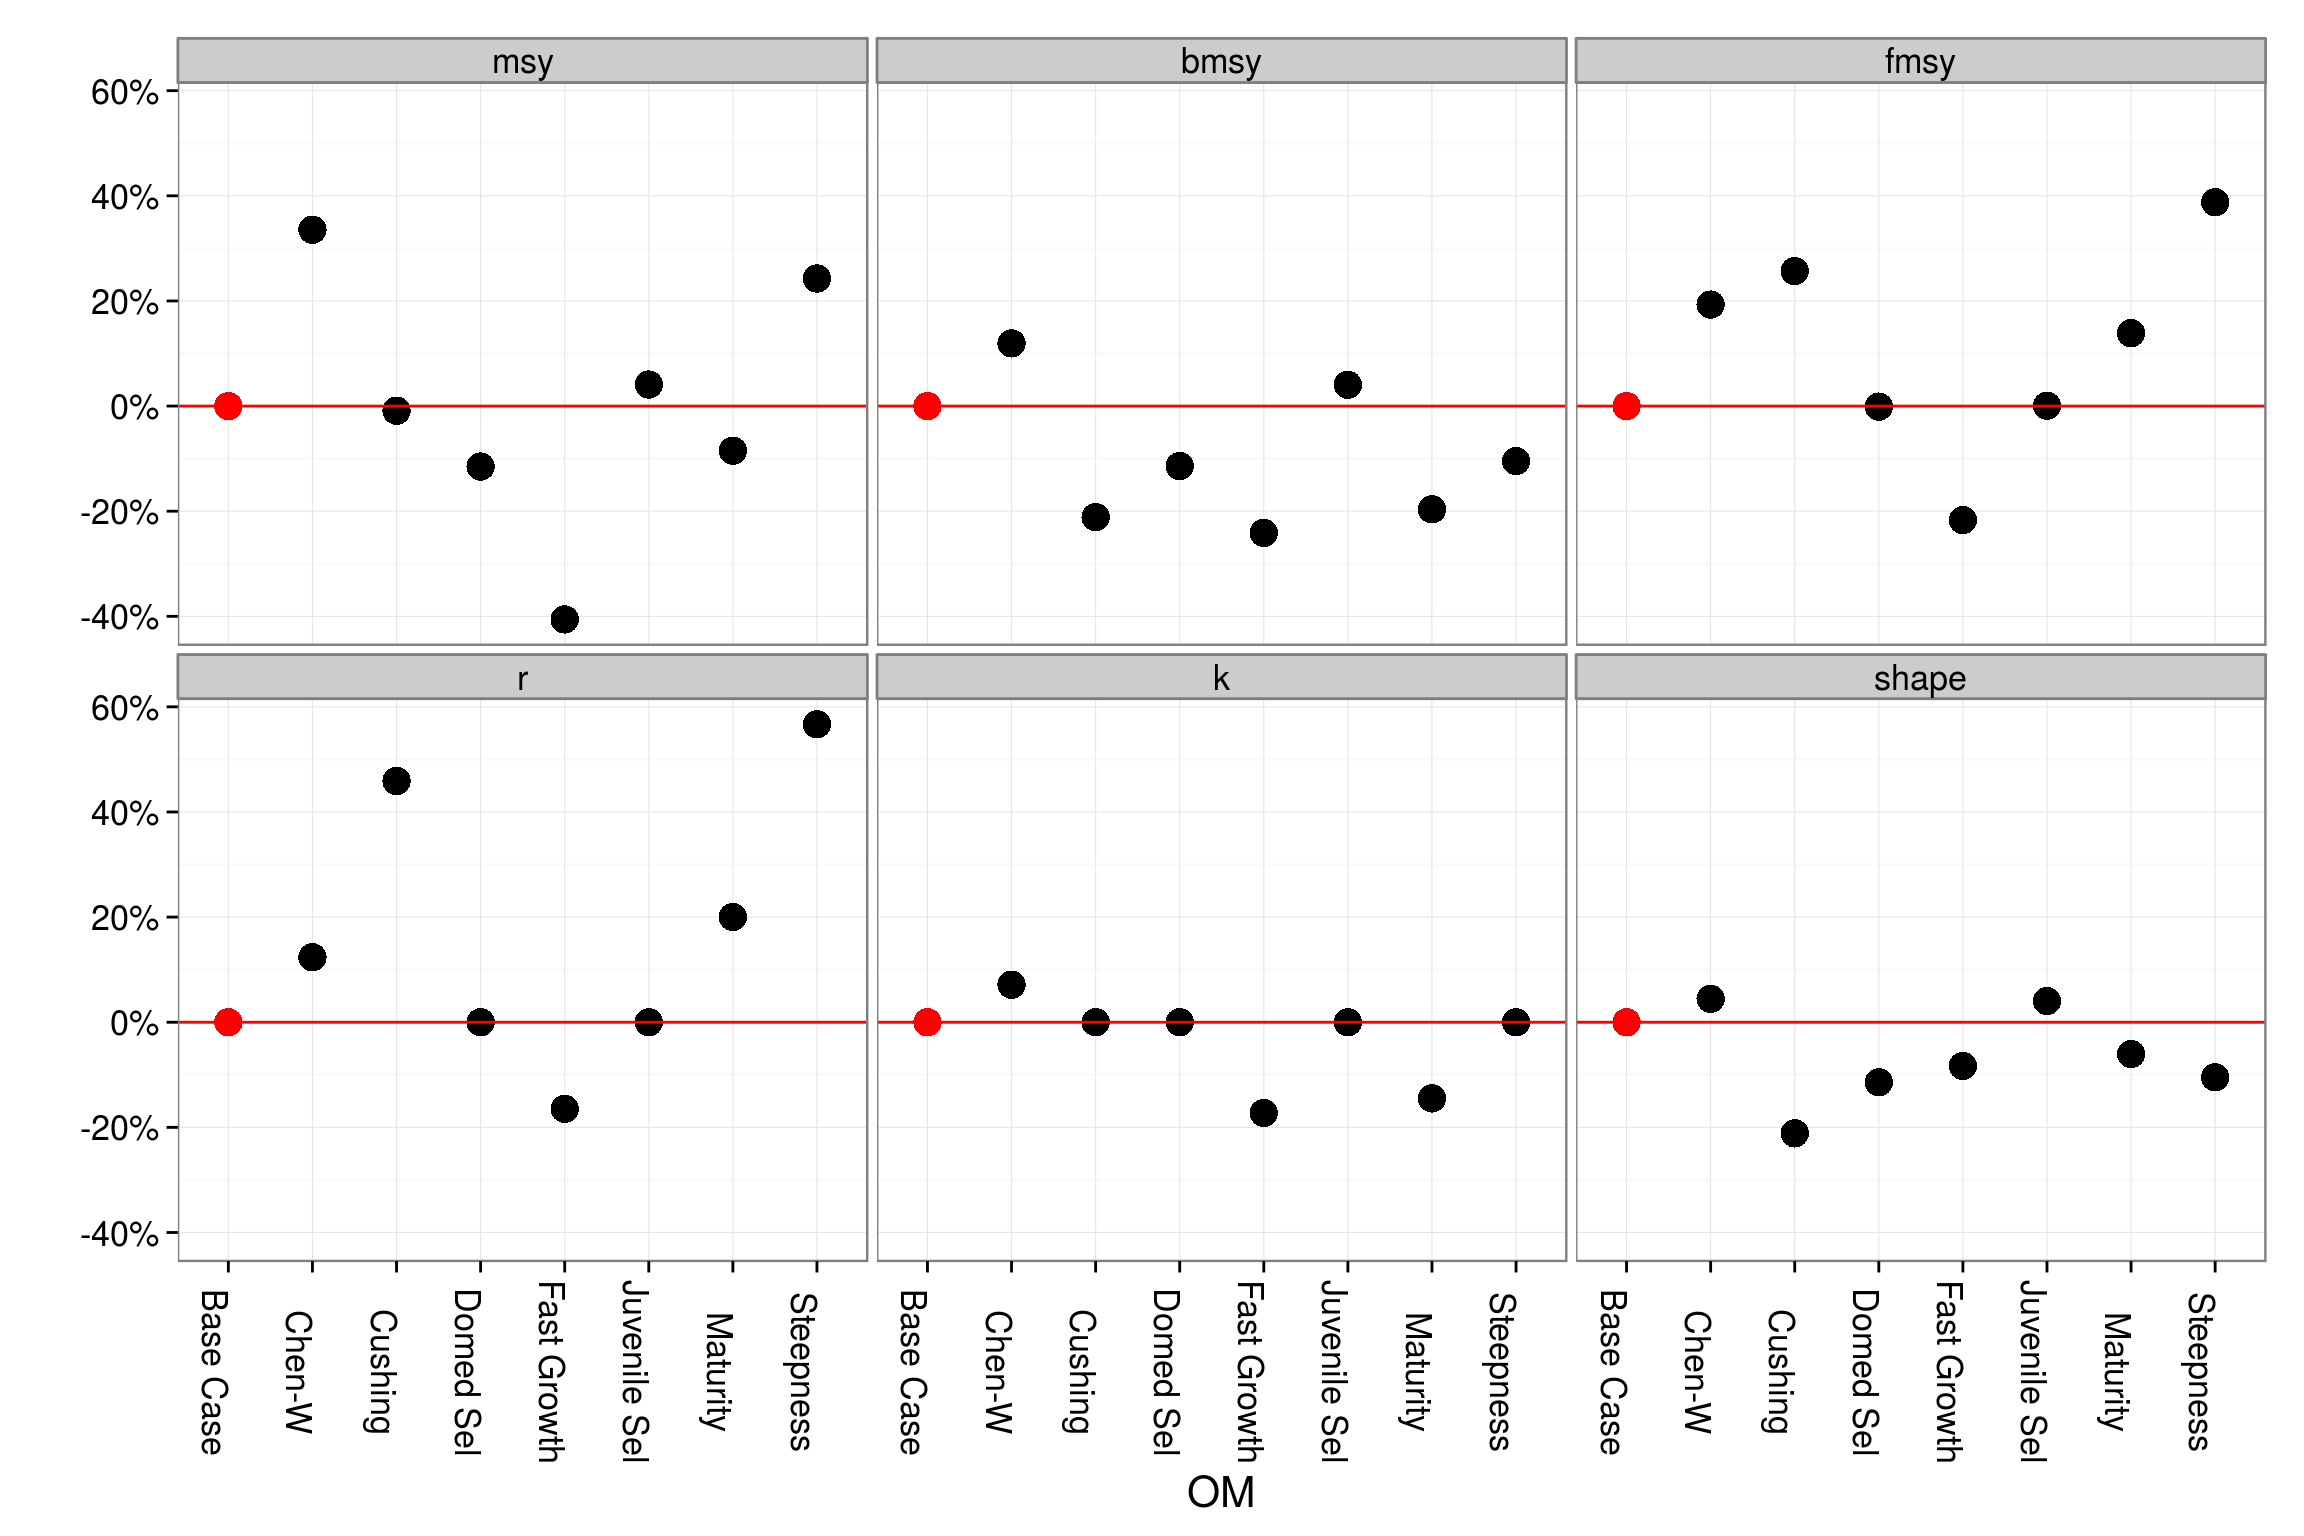
\includegraphics[width=6in]{ssOMs.png}
\caption{Population parameters and reference points by OM scenarios, values are relative to the Base Case (red).}
\label{fig:popPar}
\end{figure*}
%\end{landscape}


\begin{figure*}[htbp]
\centering
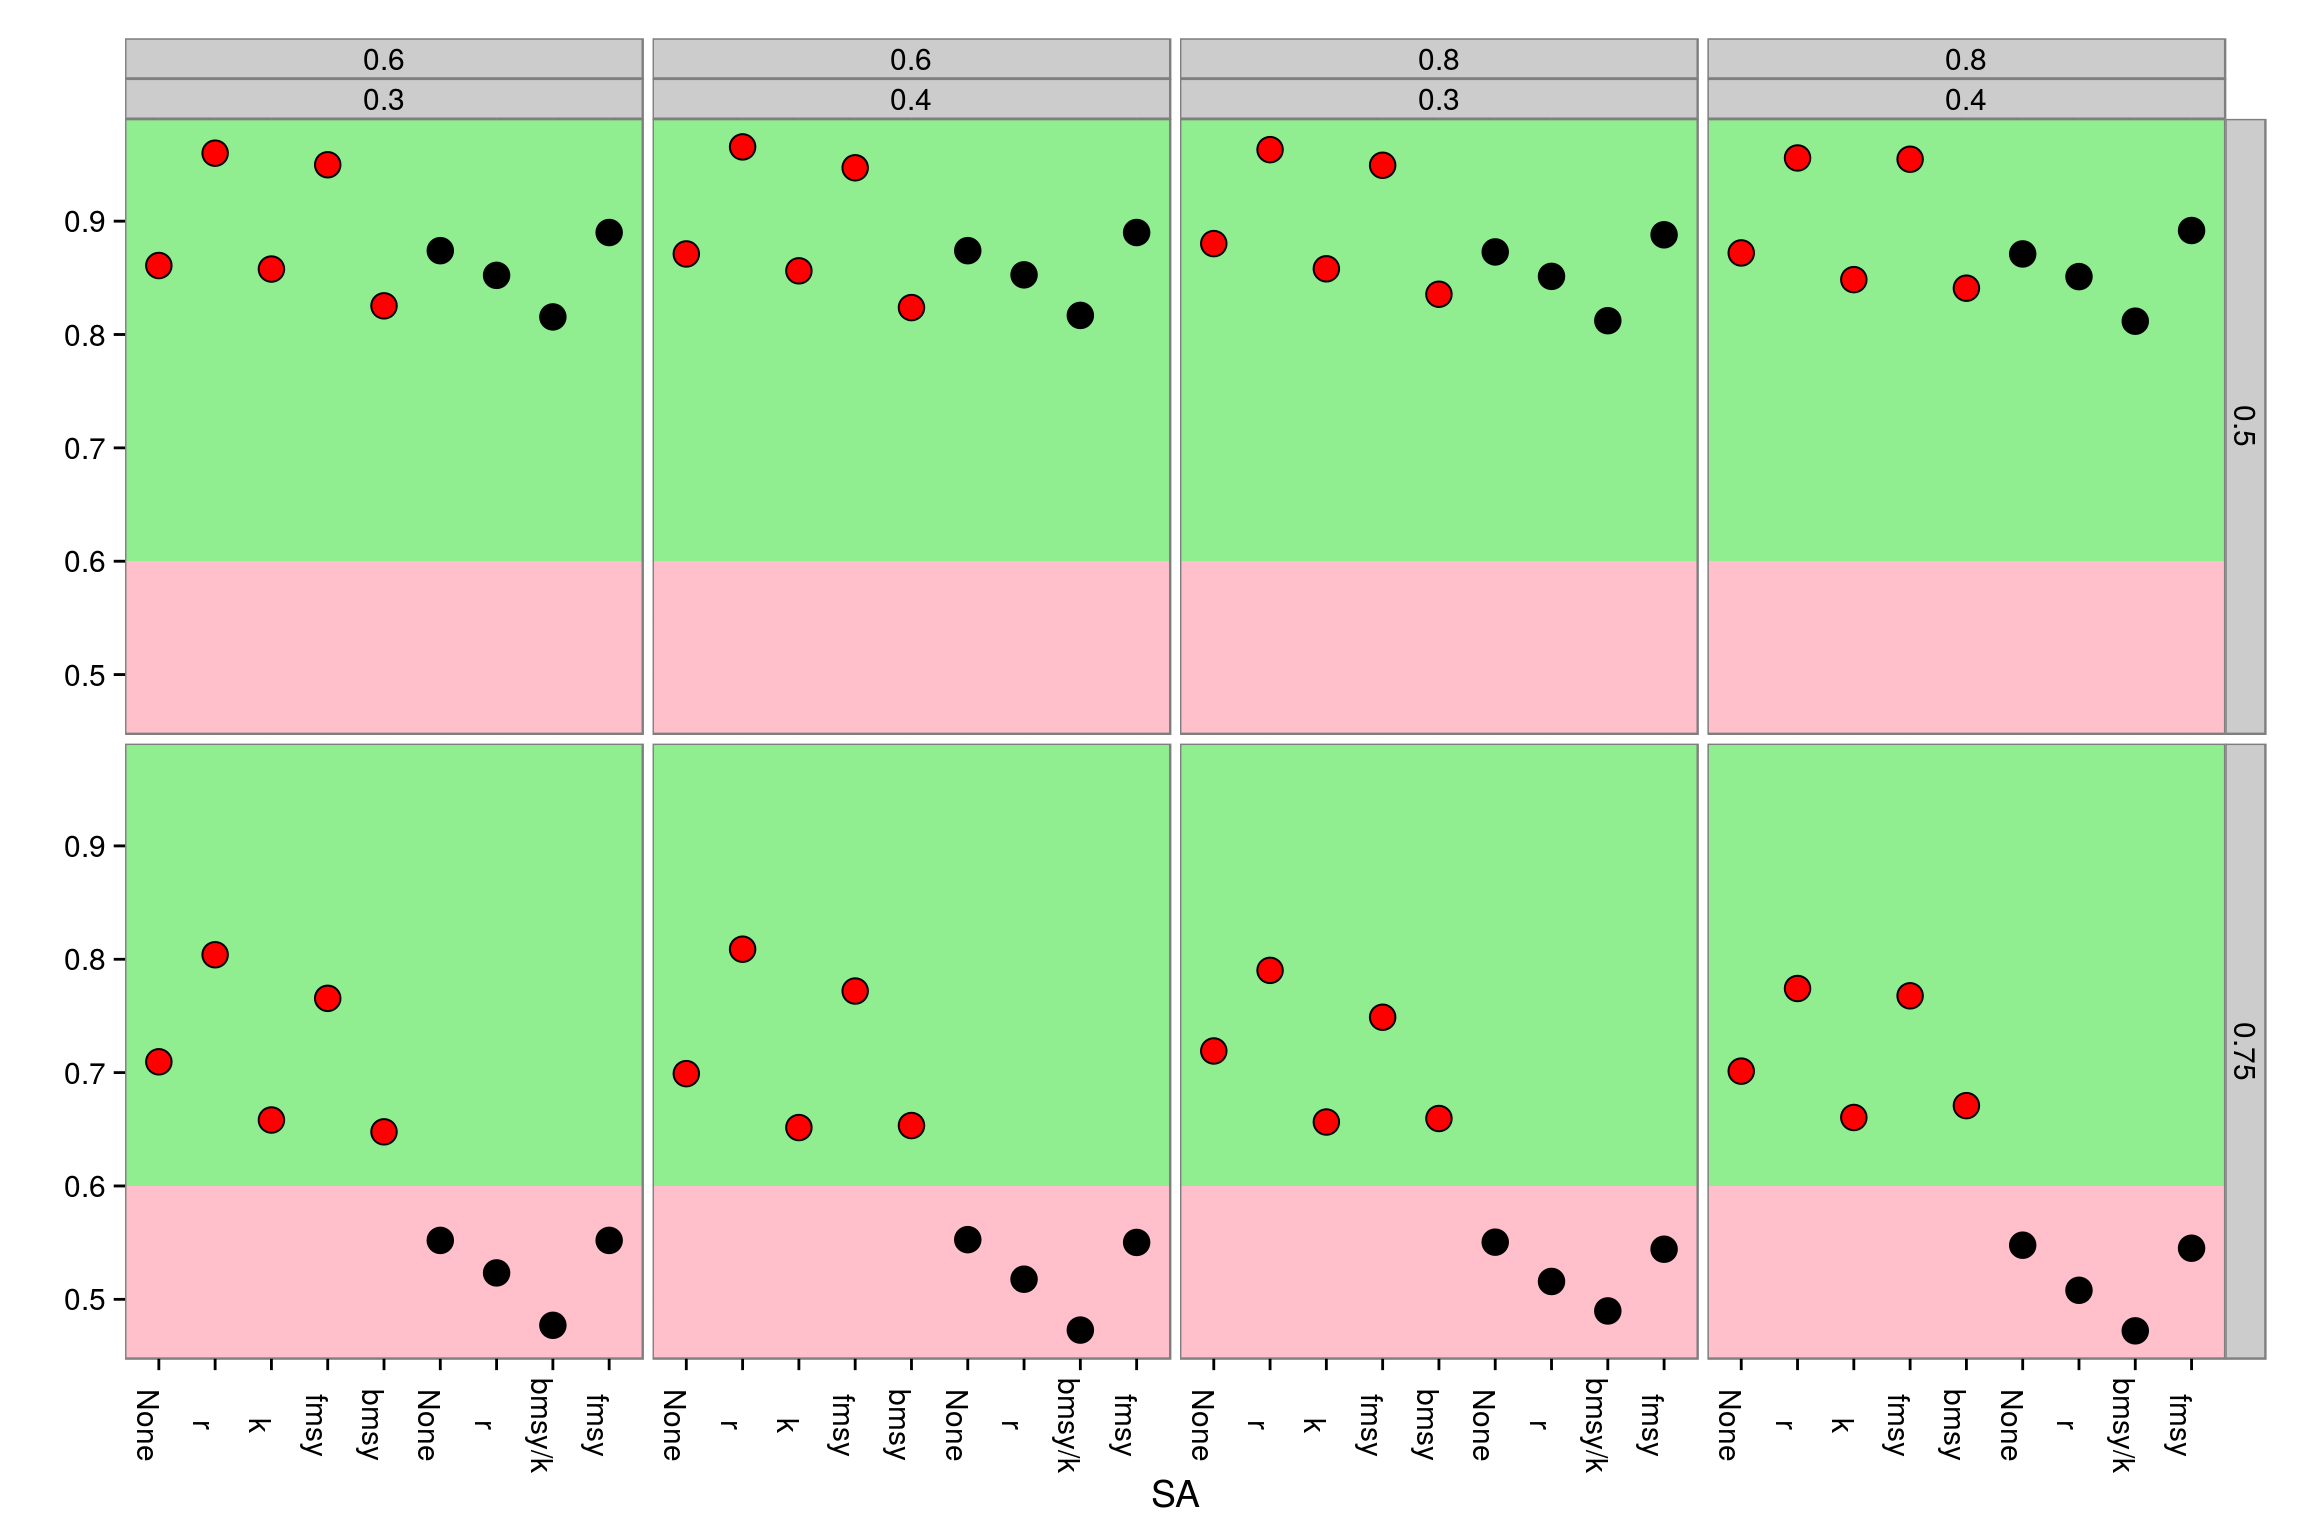
\includegraphics[width=6in]{ssGreen.png}
\caption{Probability of being in the green quadrant of the Kobe phase plot, by biomass thresholds and limits as a proportion of $B_{MSY}$ (columns) and fishing mortality targets as a proportion of $F_{MSY}$(rows)}
\label{fig:ssGreen}
\end{figure*}

%\begin{landscape}
\begin{figure*}[htbp]
\centering
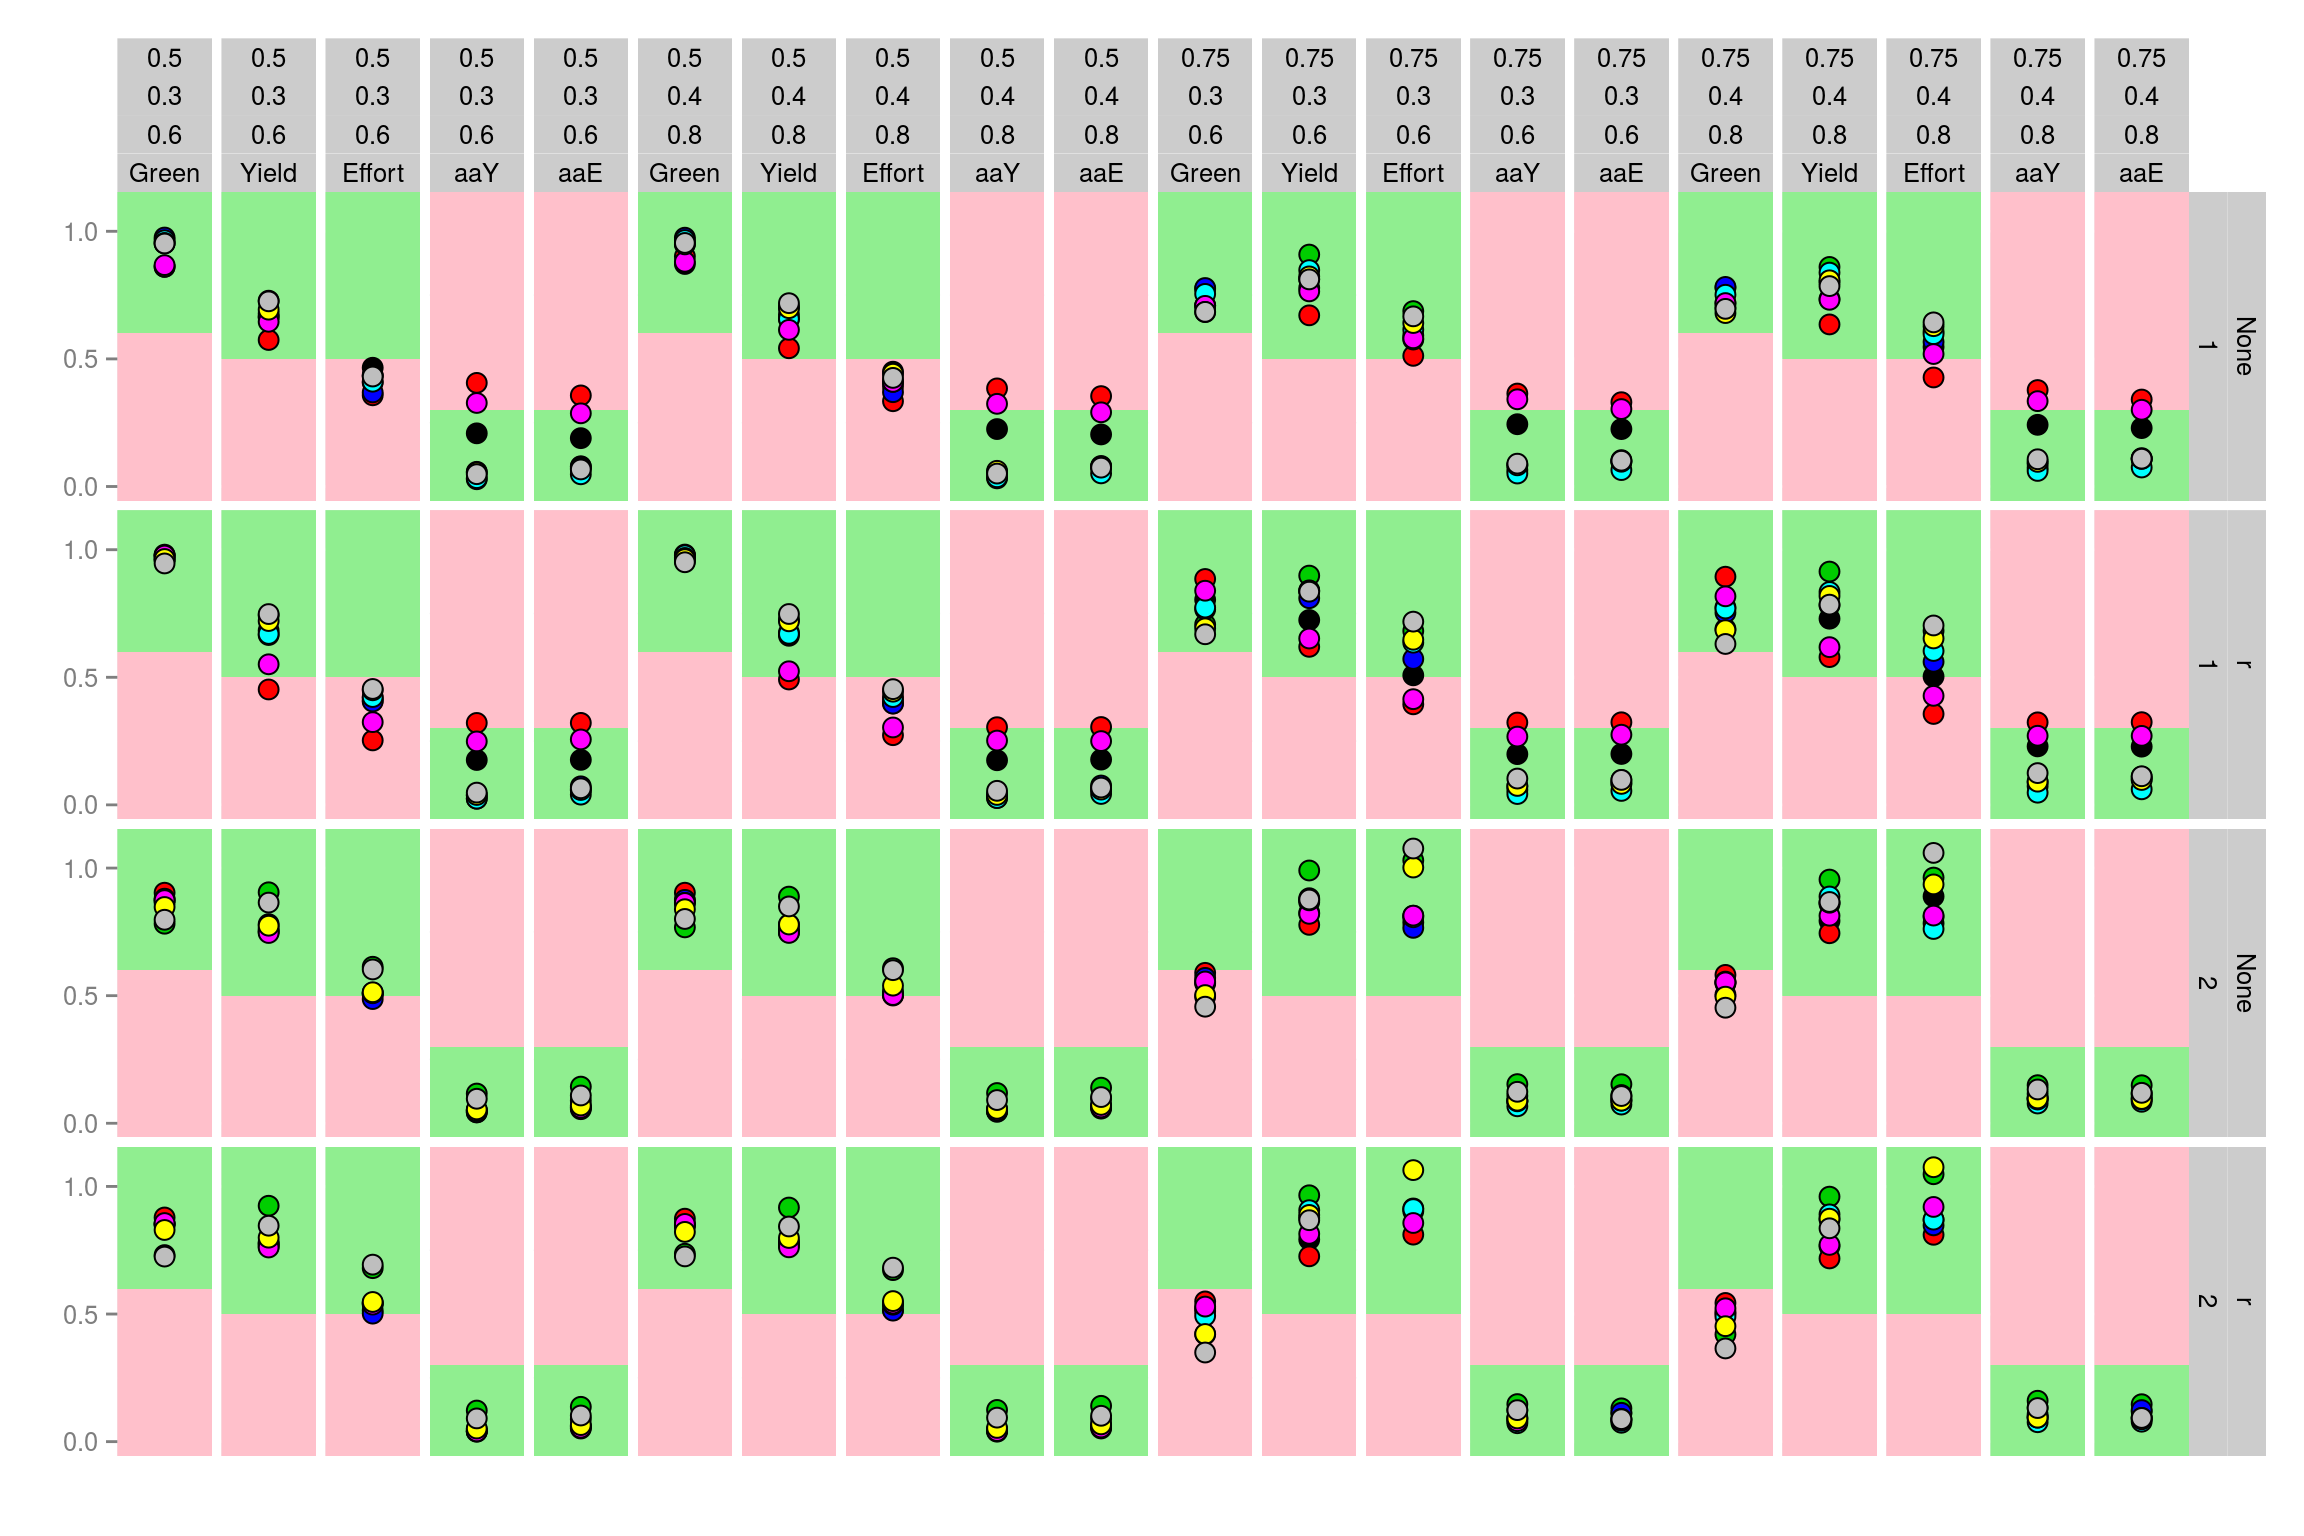
\includegraphics[width=6in]{ssSmry.png}
\caption{Summary.}
\label{fig:smry}
\end{figure*}
%\end{landscape}

These describe the input-output characteristic i.e. of the system, i.e. catch as a function of effort

